\documentclass[landscape,9pt]{beamer}

%% define basic beamer themes 
\usetheme{Boadilla}
\usecolortheme{whale} 
\usefonttheme[onlymath]{serif}

% Settings for tikz (to make graphs)
\usepackage{tikz,verbatim,graphicx}
\usetikzlibrary{shapes,arrows,arrows.meta,decorations.pathreplacing,positioning}

%%%%%%% creates logs
\newcommand{\MRC}{
\logo{
\includegraphics[height=.37cm]{MRC.png}} 
\setbeamertemplate{sidebar right}{% 
  \vfill%
  \llap{\insertlogo\hskip0.0cm}%
}
}

\newcommand{\UCL}{
\logo{
\includegraphics[height=.37cm]{UCL.jpg}} 
\setbeamertemplate{sidebar right}{% 
  \vfill%
  \llap{\insertlogo\hskip0.0cm}\vskip0.015cm%
}
}

\newcommand{\Bristol}{
\logo{
\includegraphics[height=.37cm]{Bristol.png}}
\setbeamertemplate{sidebar right}{% 
  \vfill%
  \llap{\insertlogo\hskip0.02cm}\vskip0.02cm%
}
}

\newcommand{\Sheffield}{
\logo{\includegraphics[height=.39cm]{Sheffield.jpg}}
\setbeamertemplate{sidebar right}{% 
  \vfill%
  \llap{\insertlogo\hskip0.0cm}\vskip0.015cm%
}
}

\newcommand{\Sickkids}{
\logo{\includegraphics[height=.39cm]{Sickkids.png}}
\setbeamertemplate{sidebar right}{% 
  \vfill%
  \llap{\insertlogo\hskip0.0cm}\vskip0.015cm%
}
}

\newcommand{\nologo}{
\logo{}
}

%% This creates a counter to get the first & last frame of each part
%% source: http://tex.stackexchange.com/questions/73142/how-can-i-get-the-first-and-the-last-frame-of-an-part-in-beamer-class
\usepackage{etoolbox}
\makeatletter
\newcount\beamer@partstartframe
\beamer@partstartframe=1
\apptocmd{\beamer@part}{\addtocontents{nav}{\protect\headcommand{%
        \protect\beamer@partframes{\the\beamer@partstartframe}{\the\c@framenumber}}}}{}{}
\apptocmd{\beamer@part}{\beamer@partstartframe=\c@framenumber\advance\beamer@partstartframe by1\relax}{}{}
\AtEndDocument{\immediate\write\@auxout{\string\@writefile{nav}%
        {\noexpand\headcommand{\noexpand\beamer@partframes{\the\beamer@partstartframe}{\the\c@framenumber}}}}}{}{}
\def\beamer@startframeofpart{1}
\def\beamer@endframeofpart{1}
\def\beamer@partframes#1#2{%
  \ifnum\c@framenumber<#1%
  \else%
    \ifnum\c@framenumber>#2%
    \else%
      \gdef\beamer@startframeofpart{#1}%
      \gdef\beamer@endframeofpart{#2}%
    \fi%
  \fi%
}
\newcommand\insertpartstartframe{\beamer@startframeofpart}
\newcommand\insertpartendframe{\beamer@endframeofpart}
\makeatother

%%% include replacement file beamerbaseframe.sty in working dir - 
%%% fixes bug with wrong frame number for fragile slides.
\usepackage{beamerbaseframe}

\PassOptionsToPackage{pdftex,usenames,dvipsnames}{color}
\bibliographystyle{unsrt}
\usepackage{amssymb,amsmath,multirow,colortbl,graphics,bm,inconsolata,marvosym}
\usepackage[normalem]{ulem}
\usepackage[abs]{overpic}		% Allows over pictures in frame
\usepackage{xspace} %% solves space annoyance with \winbugs macro
\usepackage{pstricks}
\usepackage[position=top]{subfig}
\usepackage{animate,framed,tabto,verbatim}
\usepackage{inputenc}
\usepackage{graphicx,mathrsfs,bibentry,chngcntr,booktabs,fancyvrb}
\usepackage[authoryear]{natbib}

% To format computer code
\usepackage{listings}
\lstset{basicstyle=\ttfamily\fontsize{6}{7}\selectfont,breaklines=true,tabsize=2,
keywords={},linewidth=1\textwidth,backgroundcolor=\color{black!5}} 

\raggedright %no right-justify
\setlength{\parskip}{3pt}

\newenvironment{shitemize}{\begin{itemize}
\setlength{\parskip}{0pt}
\setlength{\itemsep}{2pt}
\setlength{\parsep}{0pt}
}{\end{itemize}}

\newcommand{\Sum}{\displaystyle \sum}
\newcommand{\bi}{\begin{itemize}}
\newcommand{\ei}{\end{itemize}}

\newcommand{\winbugs}{{\texttt{WinBUGS}}\xspace}
\newcommand{\openbugs}{{\texttt{OpenBUGS}}\xspace}
\newcommand{\jags}{{\texttt{JAGS}}\xspace}
\newcommand{\bugs}{{\texttt{BUGS}}\xspace}

\newcommand{\tca}[1]{\textcolor{black}{#1}}
\newcommand{\tcb}[1]{\textcolor{black}{#1}}

\newcommand{\bpi}{\mbox{\boldmath $ \pi $}}
\newcommand{\bLambda}{\mbox{\boldmath $ \Lambda $}}
\newcommand{\bc}{\mbox{\boldmath $ c $}}
\newcommand{\bb}{\mbox{\boldmath $ b $}}
\newcommand{\bC}{\mbox{\boldmath $ C $}}

\newcommand{\distspace}{ \,\,\,\,\,}
\newcommand{\ie}{ {\hspace{-1.5mm}\it i.e.} }
\newcommand{\eg}{ {\hspace{-1.5mm}\it e.g.} }

\newcommand{\EXP}{\ensuremath{\mathbb{E}}}
\newcommand{\VAR}{\ensuremath{\mathbb{V}}}
\newcommand{\COV}{\ensuremath{\mathbb{V}}}
%\newcommand{\E}{\mbox{\boldmath $ E $}}
\newcommand{\E}{\mbox{E}}

\newcommand{\pd}[1]{\parbox[c]{1.2 cm}{\fontsize{6}{5} \selectfont \centering #1}}
\newcommand{\ps}[1]{\parbox[c]{1 cm}{\fontsize{6}{5} \selectfont \centering #1}}
\renewcommand{\b}{\mbox{B}}
\newcommand{\bcea}{\texttt{BCEA}\xspace}
\newcommand{\R}{\texttt{R}\xspace}
\newcommand{\hs}{\hspace{5pt}}
\newcommand{\mytilde}{{\raise.17ex\hbox{$\scriptstyle\mathtt{\sim}$}}\xspace}
\newcommand{\logit}{\mathop{\mathrm{logit}}}

\newcommand{\bx}{\mbox{$\mathbf{x}$}}
\newcommand{\xvec}{\mbox{$\bx_1,\ldots,\bx_n$}}
\newcommand{\yxvec}{\mbox{$y_1=f(\bx_1),\ldots,y_n=f(\bx_n)$}}
\newcommand{\by}{\mbox{$\mathbf{y}$}}
\newcommand{\bh}{\mbox{$\mathbf{h}$}}
\newcommand{\bt}{\mbox{$\mathbf{t}$}}
\newcommand{\bbeta}{\mbox{\boldmath{$\beta$}}\unboldmath}
\newcommand{\bdelta}{\mbox{\boldmath{$\delta$}}\unboldmath}
\newcommand{\bphi}{\mbox{\boldmath{$\phi$}}\unboldmath}
\newcommand{\btheta}{\mbox{\boldmath{$\theta$}}\unboldmath}
\newcommand{\bo}[1]{\mbox{$\mathbf{#1}$}}
\newcommand{\yxpvec}{\mbox{$y_1'=\eta(\bx_1'),\ldots,y_{n'}'=\eta(\bx_{n'}')$}}
\newcommand{\xpvec}{\mbox{$\bx_1',\ldots,\bx_{n'}'$}}
\newcommand{\ri}{\mbox{$^{131}I$} }
\newcommand{\bZ}{\mbox{$\bm{Z}$}}
\newcommand{\T}{\mbox{$\bm{\theta}$}}
\newcommand{\X}{\mbox{$\bm{X}$}}
\newcommand{\x}{\mbox{$\bm{x}$}}
%\newcommand{\btheta}{\mbox{$\bm{\theta}$}}
\newcommand{\M}{\mbox{$\NB(d,\bm\theta)$}}
\newcommand{\NB}{\mbox{NB}}
\newcommand{\nb}{\mbox{$\mathbf{nb}$}}
\newcommand{\EVPI}{\mbox{$\mbox{EVPPI}$}}
\newcommand{\EVSI}{\mbox{EVSI}}
\newcommand{\Cov}{\mbox{$\mbox{Cov}$}}
\newcommand{\bX}{\mbox{$\bm{X}$}}
\newcommand{\K}{\mbox{$\mathbf{K}$}}
\newcommand\independent{\protect\mathpalette{\protect\independenT}{\perp}}
\def\independenT#1#2{\mathrel{\rlap{$#1#2$}\mkern4mu{#1#2}}}
\newcommand{\notindependent}{%
\mathrel{\ooalign{$\independent$\cr\kern3pt$/$}}}
\newcommand{\Data}{%
\mathrm{Data}}
\newcommand{\dd}{%
\mathrm{d}}
\newcommand{\N}{\mbox{${NB}$}}

\newenvironment{shenumerate}{\begin{enumerate}
\setlength{\parskip}{0pt}
\setlength{\itemsep}{2pt}
\setlength{\parsep}{0pt}
}{\end{enumerate}}

%% Books to reference
\newcommand{\bmhe}{\footnotesize  \textit{Bayesian Methods in Health Economics}}
\newcommand{\bugsbook}{\footnotesize  \textit{The \texttt{BUGS} Book}}
\newcommand{\bceabook}{\footnotesize  Baio et al (2017). \textit{Bayesian Cost-Effectiveness Analysis with the \texttt{R} package \texttt{BCEA}}}
\newcommand{\esdmh}{\footnotesize Welton et al (2012). \textit{Evidence Synthesis for Decision Making in Healthcare}}
\newcommand{\gelmanhill}{\footnotesize Gelman and Hill (2007). \textit{Data Analysis Using Regression and Multilevel/Hierarchical Models}}

\definecolor{rpurple}{rgb}{0.627, 0.125, 0.941}
\setbeamerfont{alerted text}{shape=\itshape}
\setbeamerfont{local structure}{shape=\slshape}
\setbeamercolor{alerted text}{fg=rpurple!80!black}
\setbeamercolor{alerted text}{fg=rpurple!80!black}

%% Defines a few new colors and commands to use them easily
\definecolor{myblue}{rgb}{0.14, 0.34, 0.55}
\definecolor{orange}{rgb}{1, 0.5, 0}
\definecolor{olive}{rgb}{.2, .31, .09}
\newcommand{\myblue}{\color{myblue}}
\newcommand{\orange}{\color{orange}}
\newcommand{\olive}{\color{olive}}
\renewcommand{\red}{\color{red}}
\renewcommand{\blue}{\color{blue}}
\renewcommand{\black}{\color{black}}
\renewcommand{\white}{\color{white}}
\renewcommand{\gray}{\color{gray}}
\newrgbcolor{amber}{1.0, 0.75, 0.0}
\definecolor{darkgrey}{rgb}{.83 .83 .83}
\newcommand\darkgrey{\color{darkgrey}}

\usepackage{hyperref}
\hypersetup{colorlinks=true,urlcolor=myblue,linkcolor=}

\setbeamertemplate{navigation symbols}{}

\setbeamerfont{footnote}{size=\tiny}
\addtobeamertemplate{footnote}{}{\vspace{1ex}}

\setbeamerfont{itemize/enumerate body}{size*={9}{11}}
\setbeamerfont{itemize/enumerate subbody}{size*={8}{10}}
\setbeamerfont{itemize/enumerate subsubbody}{size*={7}{9}}

\title{Aspects of Decision Making in Cost-effectiveness Modelling}
\part{University of Oxford}
\date{24th November 2022}
\author{Nathan Green (n.green@ucl.ac.uk)\\
(with thanks to Gianluca Baio, Chris Jackson, Nicky J.~Welton, Mark Strong, Anna Heath)}

\begin{document}
\frame{\titlepage}

\date{Day 1}

\addtocounter{part}{-1}			% Labels the first part as 0 --- preliminaries
\renewcommand{\partname}{ }		% Remove the label "Part"
%% customised footline for the preliminaries
\makeatletter
\setbeamertemplate{footline}{%
  \leavevmode%
  \hbox{%
  \begin{beamercolorbox}[wd=.35\paperwidth,ht=2.25ex,dp=1ex,center]{title in head/foot}%
    \usebeamerfont{title in head/foot}\insertshorttitle
  \end{beamercolorbox}%
  \begin{beamercolorbox}[wd=.10\paperwidth,ht=2.25ex,dp=1ex,center]{date in head/foot}% original wd=.15
    \usebeamerfont{date in head/foot}\insertshortdate{}
  \end{beamercolorbox}%
  \begin{beamercolorbox}[wd=.40\paperwidth,ht=2.25ex,dp=1ex,center]{section in head/foot}% original wd=.35
    \usebeamerfont{section in head/foot} \insertshortpart 
  \end{beamercolorbox}%
  \begin{beamercolorbox}[wd=.15\paperwidth,ht=2.25ex,dp=1ex,center]{date in head/foot}%
%    \insertframenumber{}\hspace*{1ex}(\insertpartstartpage--\insertpartendpage)
%    \insertframenumber{}\hspace*{1ex}(\insertpartstartframe--\insertpartendframe)
  \end{beamercolorbox}}%
  \vskip0pt%
}
\makeatother
\part[Preliminaries]{Preliminaries} \frame{\partpage} 

\begin{frame}
\frametitle{University College London}
\begin{tabular}{lcr}
\begin{minipage}[l]{5.0cm}
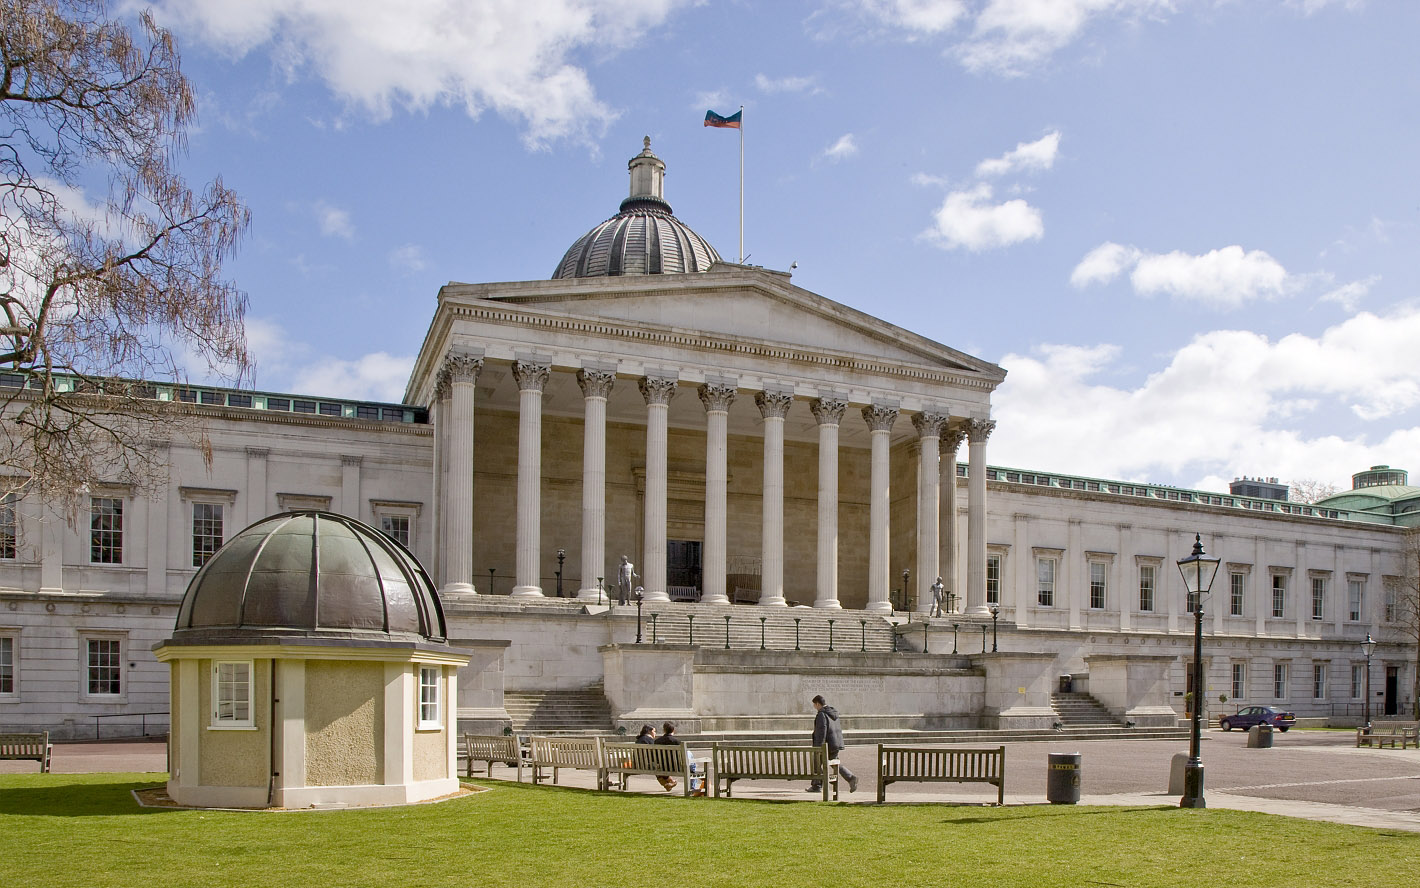
\includegraphics[height=3.8cm]{ucl_building}
\end{minipage} & &
\begin{minipage}[r]{6.5cm}
\begin{itemize}
\item UCL was rated 2nd in the UK for research power in the Research Excellence Framework 2021
\item UCL is ranked 8th in the 2022 QS World University Rankings
\item The Department of Statistical Science has played a major role in the development of the subject ever since its foundation in 1911 as the Department of Applied Statistics
\end{itemize}
\end{minipage}
\end{tabular}
\end{frame}

\begin{frame}%[noframenumbering]
\frametitle{Objectives}

\only<1>{
\begin{tabular}{lcr}
\begin{minipage}[l]{5.0cm}
\textbf{Lectures}\\
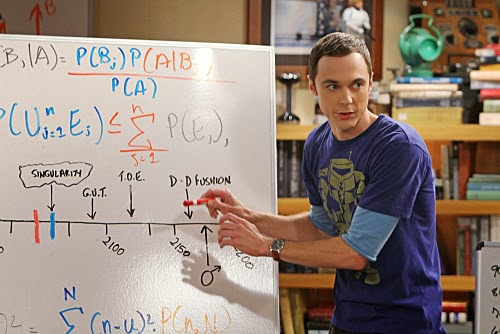
\includegraphics[height=3.8cm]{Lecture}
\end{minipage} & &
\begin{minipage}[r]{6.5cm}
\begin{itemize}
	\item Introduction to \alert{Health economics modelling}
	\begin{itemize}
		\item Decision trees
		\item Markov models
	\end{itemize}
	\vspace{10pt}
	\item Introduction to sensitivity analyses
	\begin{itemize}
		\item Deterministic
		\begin{itemize}
			\item One-way \& multi-way
			\item Scenario
		\end{itemize}
		\item Probabilistic
	\end{itemize}  
\end{itemize}
\end{minipage}
\end{tabular}}

\only<2>{
\begin{tabular}{lcr}
\begin{minipage}[l]{5.0cm}
\textbf{Computer practicals}\\
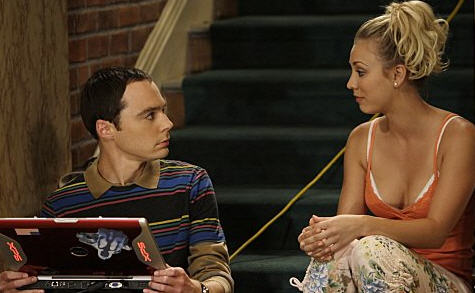
\includegraphics[height=3.5cm]{Practical}
\end{minipage} & &
\begin{minipage}[r]{6.5cm}
\begin{itemize}
\item Emphasis on practical examples
\begin{itemize}
\item Decision tree and Markov models 
\item using \texttt{R} programming language
\end{itemize}
\end{itemize}
\end{minipage} 
\end{tabular}}
\end{frame}

\frame{
\frametitle{Timetable}
\begin{itemize}
\item 2:00-3:00 Health Economics modelling lecture
\item 3:00 - 3:45 Decision tree and Markov model practical
\item BREAK
\item 3:50 - 4:20 Sensitivity analysis lecture
\item 4:20-5:00 Sensitivity analysis practical
\end{itemize}
}

\begin{frame}%[noframenumbering]
\frametitle{More Bayesian Health Economics...}

\begin{tabular}{lcr}
\begin{minipage}[l]{5.0cm}
\textbf{Books}\\

\includegraphics[height=3.8cm]{bcea_book}
\includegraphics[height=3.8cm]{bmhe_book}
\end{minipage} & &
\begin{minipage}[r]{6.5cm}
\begin{itemize}
\item This course is only a small part of an \alert{annual week-long summer school}
\begin{itemize}
\item usually in Florence, Italy
\end{itemize}
\item Several books available
\item Edition two of BCEA book in the pipeline and a Health Economic in R book close to being finished!
\end{itemize}

\end{minipage}
\end{tabular}
\end{frame}



% This changes the default setting and uses arabic instead of Roman numbers for the parts (lectures)
% source: https://tex.stackexchange.com/questions/65560/changing-of-the-numbering-of-parts-in-beamer
\setbeamertemplate{part page}
{
  \begin{centering}
    {\usebeamerfont{part name}\usebeamercolor[fg]{part name}\partname~\insertpartnumber}
    \vskip1em\par
    \begin{beamercolorbox}[sep=10pt,center,rounded=true]{part title}
      \usebeamerfont{part title}\insertpart\par
    \end{beamercolorbox}
  \end{centering}
}
%% customised footline (same as before but now also includes the lecture number in the footer
\makeatletter
\setbeamertemplate{footline}{%
  \leavevmode%
  \hbox{%
  \begin{beamercolorbox}[wd=.35\paperwidth,ht=2.25ex,dp=1ex,center]{title in head/foot}%
    \usebeamerfont{title in head/foot}\insertshorttitle
  \end{beamercolorbox}%
  \begin{beamercolorbox}[wd=.10\paperwidth,ht=2.25ex,dp=1ex,center]{date in head/foot}% original wd=.15
    \usebeamerfont{date in head/foot}\insertshortdate{}
  \end{beamercolorbox}%
  \begin{beamercolorbox}[wd=.40\paperwidth,ht=2.25ex,dp=1ex,center]{section in head/foot}% original wd=.35
    \usebeamerfont{section in head/foot} \insertpartnumber.\ \insertshortpart 
  \end{beamercolorbox}%
  \begin{beamercolorbox}[wd=.15\paperwidth,ht=2.25ex,dp=1ex,center]{date in head/foot}%
%    \insertframenumber{}\hspace*{1ex}(\insertpartstartpage--\insertpartendpage)
    \insertframenumber{}\hspace*{1ex}(\insertpartstartframe--\insertpartendframe)
  \end{beamercolorbox}}%
  \vskip0pt%
}
\makeatother

\renewcommand{\partname}{Lecture}	% Changes the label "Part" to "Lecture"
\addtocounter{framenumber}{-3}

%\part[Introduction to health economic evaluation]{Introduction to health economic evaluations} \frame{\partpage} \UCL
%%%%%\setbeamerfont{itemize/enumerate body}{size*={9}{11}}
%%%%\setbeamerfont{itemize/enumerate subbody}{size*={8}{10}}
%%%%\setbeamerfont{itemize/enumerate subsubbody}{size*={7}{9}}

\frame{%
\frametitle{Summary}
\begin{itemize}
\item Health economic evaluation
\begin{itemize}
\item What is health economics?
\item Why do we need health economics?
\end{itemize}
\item A framework for health economic evaluation
\begin{itemize}
\item Statistical modelling
\item Economic modelling
\item Decision analysis
\item Uncertainty analysis
\end{itemize}
\item Standard vs Bayesian HTA
\begin{itemize}
\item Two-stage vs integrated approach
\end{itemize}
\item Decision-making
\begin{itemize}
\item Cost-effectiveness plane
\item ICER
\item EIB
\end{itemize}
\end{itemize}

\vfill
\begin{block}{\footnotesize References}
\bmhe, chapter 1.\\
\bceabook
\end{block}

}

\frame{
\setbeamerfont{itemize/enumerate body}{size*={5}{6}}
\setbeamerfont{itemize/enumerate subbody}{size*={4}{5}}
\setbeamerfont{itemize/enumerate subsubbody}{size*={3}{4}}

\frametitle{Health technology assessment (HTA)}
\textbf{Objective}: Combine \red costs \black \& \blue benefits \black of a given intervention into a rational scheme for allocating resources
\vspace{-.4cm}
\begin{figure}
\begin{tikzpicture}%[->,>=latex,shorten >=0pt,auto,node distance=3cm,ultra thin]

\onslide<2->{\draw(-5,-1) node[align=center,rectangle,rounded corners=2ex,draw,fill=red,font=\sffamily\fontsize{9}{10}\selectfont,minimum width=2.2cm,minimum height=1cm](1){Statistical\\ model};
}
\onslide<3->{
\draw(0,-1) node[align=center,rectangle,rounded corners=2ex,draw,fill=gray,font=\sffamily\fontsize{9}{10}\selectfont,minimum width=2.2cm,minimum height=1cm](2){Economic\\ model};
}
\onslide<4->{
\draw(4,-1) node[align=center,rectangle,rounded corners=2ex,draw,fill=orange,font=\sffamily\fontsize{9}{10}\selectfont,minimum width=2.2cm,minimum height=1cm](3){Decision\\ analysis};
}
\onslide<5->{
\draw(-2.5,2) node[align=center,rectangle,rounded corners=2ex,draw,fill=blue!40,font=\sffamily\fontsize{9}{10}\selectfont,minimum width=2.2cm,minimum height=1cm](4){Uncertainty\\ analysis};
}
\onslide<2->{
\draw(-5.2,-2.7) node[align=center,rectangle,rounded corners,draw=none,font=\sffamily,text width=3cm](5){
\begin{itemize}
\item Estimates relevant \textbf{population} parameters $\bm\theta$
\item Varies with the type of available data (\& statistical approach!)
\end{itemize}
};
}
\onslide<3->{
\draw(-0.2,-2.65) node[align=center,rectangle,rounded corners,draw=none,font=\sffamily\fontsize{5}{6}\selectfont,text width=3.5cm](6){
\begin{itemize}
\item Combines the parameters to obtain a population average measure for costs and clinical benefits
\item Varies with the type of available data \& statistical model used
\end{itemize}
};
}
\onslide<4->{
\draw(3.8,-2.8) node[align=center,rectangle,rounded corners,draw=none,font=\sffamily\fontsize{5}{6}\selectfont,text width=3.4cm](7){
\begin{itemize}
\item Summarises the economic model by computing suitable measures of ``cost-effectiveness''
\item Dictates the best course of actions, given current evidence
\item Standardised process
\end{itemize}
};
}
\onslide<5->{
\draw(0.7,2.05) node[align=center,rectangle,rounded corners,draw=none,font=\sffamily\fontsize{5}{6}\selectfont,text width=4.1cm](8){
\begin{itemize}
\item Assesses the impact of uncertainty (eg in parameters or model structure) on the economic results
\item Mandatory in many jurisdictions (including NICE, in the UK)
\item Fundamentally Bayesian!
\end{itemize}
};
}
\onslide<5->{
\draw [dashed,->,>=latex,shorten >=0pt,auto,node distance=3cm,ultra thin] (1.40) -- (4.220);
\draw [dashed,->,>=latex,shorten >=0pt,auto,node distance=3cm,ultra thin] (4.320) -- (2.140);
}
\onslide<3->{
\draw [->,>=latex,shorten >=0pt,auto,node distance=3cm,ultra thin] (1.east) -- (2.west);
}
\onslide<4->{
\draw [->,>=latex,shorten >=0pt,auto,node distance=3cm,ultra thin] (2.east) -- (3.west);
}

\onslide<3->{
\draw(0.4,.15) node[align=center,rectangle,rounded corners,draw=none,font=\sffamily\fontsize{5}{6}\selectfont,text width=3.5cm](func1){
\begin{itemize}
\item[] $\myblue \Delta_e=f_e(\bm\theta)$
\item[] $\myblue \Delta_c=f_c(\bm\theta)$
\item[] $\white \ldots$
\end{itemize}
};
}

\onslide<4->{
\draw(4.1,.15) node[align=center,rectangle,rounded corners,draw=none,font=\sffamily\fontsize{5}{6}\selectfont,text width=3.5cm](func2){
\begin{itemize}
\item[] $\myblue \mbox{ICER}=g(\Delta_e,\Delta_c)$
\item[] $\myblue \mbox{EIB}=h(\Delta_e,\Delta_c;k)$
\item[] $\myblue \qquad \qquad \ldots$
\end{itemize}
};
}
\end{tikzpicture}
\end{figure}
}

\frame{
\setbeamerfont{itemize/enumerate body}{size*={5}{6}}
\setbeamerfont{itemize/enumerate subbody}{size*={4}{5}}
\setbeamerfont{itemize/enumerate subsubbody}{size*={3}{4}}

\frametitle{``Standard'' approach to HTA --- ``Two-stage''}
\begin{figure}
\begin{tikzpicture}%[->,>=latex,shorten >=0pt,auto,node distance=3cm,ultra thin]
\hspace{-.5cm}
\onslide<1->{\draw(-5,-1) node[align=center,rectangle,rounded corners=2ex,draw,fill=red,font=\sffamily\fontsize{9}{10}\selectfont,minimum width=2.2cm,minimum height=1cm](1){Statistical\\ model};
}
\onslide<1->{

\draw(0.5,-1) node[align=center,rectangle,rounded corners=2ex,draw,fill=gray,font=\sffamily\fontsize{9}{10}\selectfont,minimum width=2.2cm,minimum height=1cm](2){Economic\\ model};
}
\onslide<1->{
\draw(4,-1) node[align=center,rectangle,rounded corners=2ex,draw,fill=orange,font=\sffamily\fontsize{9}{10}\selectfont,minimum width=2.2cm,minimum height=1cm](3){Decision\\ analysis};
}
\onslide<1->{
\draw(-5,2) node[align=center,rectangle,rounded corners=2ex,draw,fill=blue!40,font=\sffamily\fontsize{9}{10}\selectfont,minimum width=2.2cm,minimum height=1cm](4){Uncertainty\\ analysis};
}
\onslide<1->{
\draw(-5.2,-2.75) node[align=center,rectangle,rounded corners,draw=none,font=\sffamily\fontsize{7}{8}\selectfont,text width=3cm](5){
\begin{itemize}
\item Estimates relevant \textbf{population} parameters $\bm\theta$
\item Varies with the type of available data (\& statistical approach!)
\end{itemize}
};
}
\onslide<1->{
\draw(0.3,-2.7) node[align=center,rectangle,rounded corners,draw=none,font=\sffamily\fontsize{7}{8}\selectfont,text width=3.5cm](6){
\begin{itemize}
\item Combines the parameters to obtain a population average measure for costs and clinical benefits
\item Varies with the type of available data \& statistical model used
\end{itemize}
};
}
\onslide<1->{
\draw(3.8,-2.85) node[align=center,rectangle,rounded corners,draw=none,font=\sffamily\fontsize{7}{8}\selectfont,text width=3.5cm](7){
\begin{itemize}
\item Summarises the economic model by computing suitable measures of ``cost-effectiveness''
\item Dictates the best course of actions, given current evidence
\item Standardised process
\end{itemize}
};
}
\onslide<1->{
\draw(-2.15,2.05) node[align=center,rectangle,rounded corners,draw=none,font=\sffamily\fontsize{7}{8}\selectfont,text width=3.7cm](8){
\begin{itemize}
\item Assesses the impact of uncertainty (eg in parameters or model structure) on the economic results
\item Mandatory in many jurisdictions (including NICE, in the UK)
\item Fundamentally Bayesian!
\end{itemize}
};
}
\onslide<1->{
%\draw [->,>=latex,shorten >=0pt,auto,node distance=3cm,ultra thin] (1.east) -- (2.west);
}
\onslide<1->{
\draw [->,>=latex,shorten >=0pt,auto,node distance=3cm,ultra thin] (2.east) -- (3.west);
}

\onslide<1->{
\draw(1.0,3.5) node[align=center,draw=none,fill=none,minimum width=.5cm,minimum height=.5cm,font=\sffamily\fontsize{6}{7}\selectfont]{\olive 1.\ Estimation (base-case)};
%\draw(4.3,3.5) node[align=center,draw=none,fill=none,minimum width=.5cm,minimum height=.5cm,font=\sffamily\fontsize{6}{7}\selectfont]{\olive 2.\ Probabilistic sensitivity analysis};
\draw(1.8,3) node[align=center,draw,fill=none,minimum width=.5cm,minimum height=.5cm,font=\sffamily\fontsize{6}{7}\selectfont](9){$\theta$};
\draw(1.8,1) node[align=center,circle,draw,fill=none,font=\sffamily\fontsize{6}{7}\selectfont](10){$y$};
\draw(.5,1) node[align=center,fill=none,minimum width=.5cm,minimum height=.5cm,font=\sffamily\fontsize{6}{7}\selectfont](11){$p(y\mid \theta)$};
\draw(.5,3) node[align=center,draw,ellipse,double,fill=none,minimum width=.3cm,minimum height=.25cm,font=\sffamily\fontsize{6}{7}\selectfont](12){$\hat\theta=f(Y)$};

\draw [->,>=latex,shorten >=0pt,auto,node distance=3cm,ultra thin] (9.south) -- (10.north);
\draw [dashed,->,>=latex,shorten >=0pt,auto,node distance=3cm,ultra thin] (11.north) -- (12.south);
\draw [dashed,->,>=latex,shorten >=0pt,auto,node distance=3cm,thin,red!60] (12.220) to [out=220,in=130] (2.120);
}

\onslide<2>{
\draw(4.3,3.5) node[align=center,draw=none,fill=none,minimum width=.5cm,minimum height=.5cm,font=\sffamily\fontsize{6}{7}\selectfont]{\olive 2.\ \textbf{Probabilistic sensitivity analysis}};
\draw(2.9,2.0) node[align=center,draw=none,fill=none,minimum width=.5cm,minimum height=.5cm,font=\sffamily\fontsize{6}{7}\selectfont,color=red]{$\Rightarrow$};
\draw(5.4,3) node[align=center,circle,draw,fill=none,font=\sffamily\fontsize{6}{7}\selectfont](13){$\theta$};
\draw(4.2,3) node[align=center,fill=none,minimum width=.5cm,minimum height=.5cm,font=\sffamily\fontsize{6}{7}\selectfont](14){$p(\theta)\red\leftrightsquigarrow\black g(\hat\theta)$};
\draw [dashed,->,>=latex,shorten >=0pt,auto,node distance=3cm,thin,blue!40] (13.south) to [out=270,in=45] (2.60);
}
\end{tikzpicture}
\end{figure}
}

\frame{
\frametitle{\only<1|handout:1>{2./3.\ Economic modelling+Decision analysis}\only<2|handout:2>{2./3./4.\ ...+\textbf{Uncertainty analysis$^*$}}}
\only<1|handout:1>{
\vspace{1.8cm}
\begin{figure}
\begin{tikzpicture}[remember picture,overlay]
\draw(0,4) node[align=center,rectangle,rounded corners,draw=none,text width=4.1cm](1){\fontsize{8}{8}\selectfont Cost-effectiveness plane};

\node{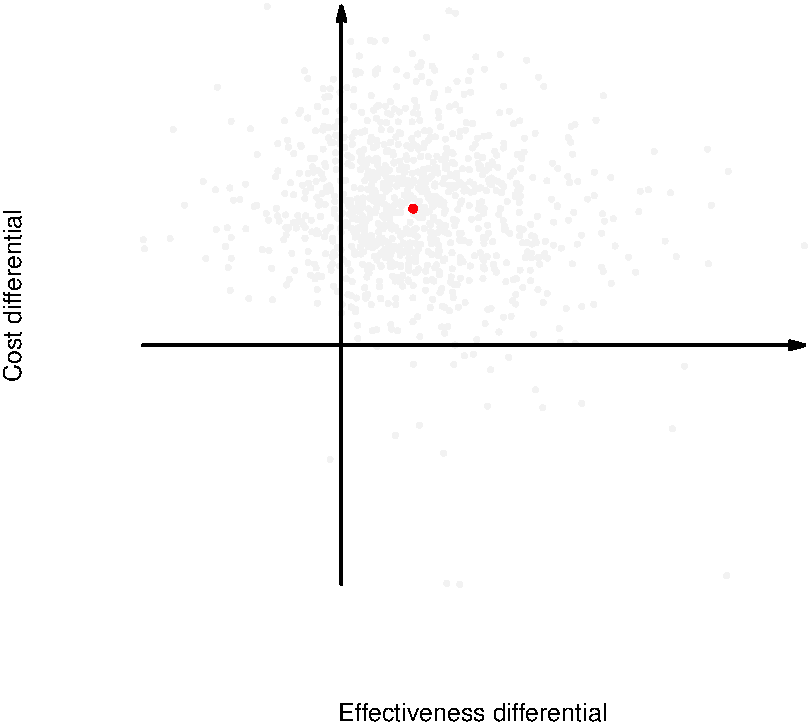
\includegraphics[scale=.55]{1.introduction-to-health-economic-evaluations/figs/CEPlane_ICER}};
\draw(3.5,-.1) node[align=center,rectangle,rounded corners,draw=none,text width=4.1cm](8){\fontsize{8}{8}\selectfont $\Delta_e$};
\draw(-.9,3.2) node[align=center,rectangle,rounded corners,draw=none,text width=4.1cm](8){\fontsize{8}{8}\selectfont $\Delta_c$};

\draw(4.5,3.5) node[align=center,rectangle,rounded corners,draw=none,text width=4.1cm](8){\fontsize{7}{8}\selectfont $\myblue \Delta_e=\red\underbrace{\myblue\mbox{E}[e \mid \hat{\bm\theta}_1]}_{\hat\mu_{e1}} \myblue - \red\underbrace{\myblue\mbox{E}[e \mid \hat{\bm\theta}_0]}_{\hat\mu_{e0}}$};
\draw(4.5,2.6) node[align=center,rectangle,rounded corners,draw=none,text width=4.1cm](8){\fontsize{7}{8}\selectfont $\myblue \Delta_c=\red\underbrace{\myblue\mbox{E}[c \mid \hat{\bm\theta}_1]}_{\hat\mu_{c1}} \myblue - \red\underbrace{\myblue\mbox{E}[c \mid \hat{\bm\theta}_0]}_{\hat\mu_{c0}}$};
\draw(2.0,1.5) node[align=center,rectangle,rounded corners,draw=none,text width=6.0cm](8){\fontsize{8}{8}\selectfont 
\begin{eqnarray*}
\mbox{ICER}&\!\!\!\!=\!\!\!\!&\frac{\mbox{E$[\Delta_c]$}}{\mbox{E$[\Delta_e]$}}=\frac{\hat\mu_{c1}-\hat\mu_{c0}}{\hat\mu_{e1}-\hat\mu_{e0}} \\
&\!\!\!\!=\!\!\!\!&\mbox{Cost per outcome}\end{eqnarray*}};
\end{tikzpicture}
\end{figure}
}

\only<2|handout:2>{
\vspace{1.8cm}
\begin{figure}
\begin{tikzpicture}[remember picture,overlay]
\draw(0,4) node[align=center,rectangle,rounded corners,draw=none,text width=4.1cm](1){\fontsize{8}{8}\selectfont Cost-effectiveness plane};
\draw(3.5,-.1) node[align=center,rectangle,rounded corners,draw=none,text width=4.1cm](8){\fontsize{8}{8}\selectfont $\Delta_e$};
\draw(-.9,3.2) node[align=center,rectangle,rounded corners,draw=none,text width=4.1cm](8){\fontsize{8}{8}\selectfont $\Delta_c$};
\node{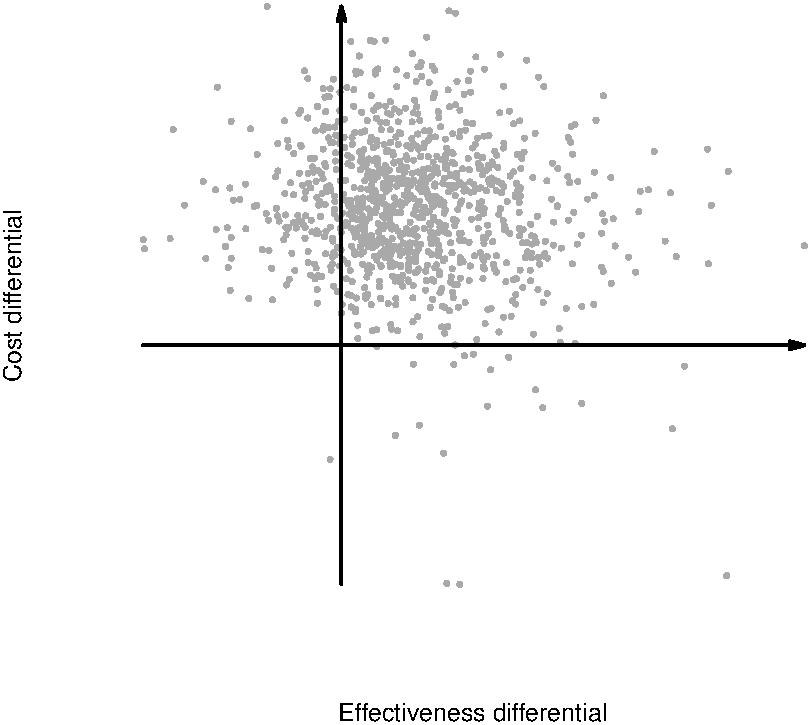
\includegraphics[scale=.55]{1.introduction-to-health-economic-evaluations/figs/CEPlane_empty}};
\draw(4.5,3.5) node[align=center,rectangle,rounded corners,draw=none,text width=4.1cm](8){\fontsize{7}{8}\selectfont $\myblue \Delta_e=\red\underbrace{\myblue\mbox{E}[e \mid \bm{\theta}_1]}_{\mu_{e1}} \myblue - \red\underbrace{\myblue\mbox{E}[e \mid \bm{\theta}_0]}_{\mu_{e0}}$};
\draw(4.5,2.6) node[align=center,rectangle,rounded corners,draw=none,text width=4.1cm](8){\fontsize{7}{8}\selectfont $\myblue \Delta_c=\red\underbrace{\myblue\mbox{E}[c \mid \bm{\theta}_1]}_{\mu_{c1}} \myblue - \red\underbrace{\myblue\mbox{E}[c \mid \bm{\theta}_0]}_{\mu_{c0}}$};
\draw(.08,1.42) node[align=center,rectangle,rounded corners,draw=none,text width=4.1cm](8){\fontsize{5}{6}\selectfont $\red \bullet$};

\draw(-4.5,-2.6) node[align=center,rectangle,rounded corners,draw=none,text width=4.1cm](8){\fontsize{7}{8}\selectfont $^*$Induced by $\myblue g(\hat{\bm\theta}_0), g(\hat{\bm\theta}_1)$};
\end{tikzpicture}
\end{figure}
}
}

\begin{frame}[label={whatswrong}]
\frametitle{What's wrong with this?...}
\begin{itemize}
\item Potential correlation between costs \& clinical benefits \hfill\scalebox{.6}{\orange[\textbf{Individual Level + Aggregated Level Data}]}
\begin{itemize}
\item Strong positive correlation --- effective treatments are innovative and result from intensive and lengthy research $\Rightarrow$ are associated with higher unit costs
\item Negative correlation --- more effective treatments may reduce total care pathway costs e.g.\ by reducing hospitalisations, side effects, etc.
\item Because of the way in which standard models are set up, bootstrapping generally only approximates the underlying level of correlation --- \textbf{\olive MCMC does a better job!}
\end{itemize}
\vspace{10pt}\pause
\item Joint/marginal normality not realistic \hfill\scalebox{.6}{\orange[\textbf{Mainly ILD}]}
\begin{itemize}
\item Costs usually skewed and benefits may be bounded in $[0;1]$
\item Can use transformation (e.g.\ logs) --- but care is needed when back transforming to the natural scale
\item Should use more suitable models (e.g.\ Beta, Gamma or log-Normal) --- \textbf{\olive generally easier under a Bayesian framework}
\item Particularly relevant in presence of partially observed data --- more on this later!
\end{itemize}
\vspace{10pt}\pause
\item Particularly as the focus is on decision-making (rather than just inference), we need to use \textbf{all} available evidence to fully characterise current uncertainty on the model parameters and outcomes \hfill\scalebox{.6}{\orange[\textbf{Mainly ALD}]}
\begin{itemize}
\item A Bayesian approach is helpful in combining different sources of information
\item \textbf{\olive Propagating uncertainty is a fundamentally Bayesian operation!}
\end{itemize}
\end{itemize}
\end{frame}


\frame{
\setbeamerfont{itemize/enumerate body}{size*={5}{6}}
\setbeamerfont{itemize/enumerate subbody}{size*={4}{5}}
\setbeamerfont{itemize/enumerate subsubbody}{size*={3}{4}}

\frametitle{Bayesian approach to HTA --- ``Integrated''}
\begin{figure}
\begin{tikzpicture}%[->,>=latex,shorten >=0pt,auto,node distance=3cm,ultra thin]
\hspace{-.5cm}
\onslide<1->{\draw(-5,-1) node[align=center,rectangle,rounded corners=2ex,draw,fill=red,font=\sffamily\fontsize{9}{10}\selectfont,minimum width=2.2cm,minimum height=1cm](1){Statistical\\ model};
}
\onslide<1->{

\draw(0.5,-1) node[align=center,rectangle,rounded corners=2ex,draw,fill=gray,font=\sffamily\fontsize{9}{10}\selectfont,minimum width=2.2cm,minimum height=1cm](2){Economic\\ model};
}
\onslide<1->{
\draw(4,-1) node[align=center,rectangle,rounded corners=2ex,draw,fill=orange,font=\sffamily\fontsize{9}{10}\selectfont,minimum width=2.2cm,minimum height=1cm](3){Decision\\ analysis};
}
\onslide<1->{
\draw(-5,2) node[align=center,rectangle,rounded corners=2ex,draw,fill=blue!40,font=\sffamily\fontsize{9}{10}\selectfont,minimum width=2.2cm,minimum height=1cm](4){Uncertainty\\ analysis};
}
\onslide<1->{
\draw(-5.2,-2.75) node[align=center,rectangle,rounded corners,draw=none,font=\sffamily\tiny,text width=3cm](5){
\begin{itemize}
\item Estimates relevant \textbf{population} parameters $\bm\theta$
\item Varies with the type of available data (\& statistical approach!)
\end{itemize}
};
}
\onslide<1->{
\draw(0.3,-2.7) node[align=center,rectangle,rounded corners,draw=none,font=\sffamily\tiny,text width=3.5cm](6){
\begin{itemize}
\item Combines the parameters to obtain a population average measure for costs and clinical benefits
\item Varies with the type of available data \& statistical model used
\end{itemize}
};
}
\onslide<1->{
\draw(3.8,-2.85) node[align=center,rectangle,rounded corners,draw=none,font=\sffamily\tiny,text width=3.5cm](7){
\begin{itemize}
\item Summarises the economic model by computing suitable measures of ``cost-effectiveness''
\item Dictates the best course of actions, given current evidence
\item Standardised process
\end{itemize}
};
}
\onslide<1->{
\draw(-2.15,2.05) node[align=center,rectangle,rounded corners,draw=none,font=\sffamily\tiny,text width=3.7cm](8){
\begin{itemize}
\item Assesses the impact of uncertainty (eg in parameters or model structure) on the economic results
\item Mandatory in many jurisdictions (including NICE, in the UK)
\item Fundamentally Bayesian!
\end{itemize}
};
}
\onslide<1->{
\draw [->,>=latex,shorten >=0pt,auto,node distance=3cm,ultra thin] (2.east) -- (3.west);
}

\onslide<1->{
\draw(2.4,3.5) node[align=center,draw=none,fill=none,minimum width=.5cm,minimum height=.5cm,font=\sffamily\fontsize{6}{7}\selectfont]{\olive \textbf{Estimation \& PSA (one stage)}};
\draw(1.8,3) node[align=center,draw,fill=none,minimum width=.5cm,minimum height=.5cm,font=\sffamily\fontsize{6}{7}\selectfont](9){$\theta$};
\draw(1.8,1) node[align=center,circle,draw,fill=none,font=\sffamily\fontsize{6}{7}\selectfont](10){$y$};
\draw(.5,1) node[align=center,fill=none,minimum width=.5cm,minimum height=.5cm,font=\sffamily\fontsize{6}{7}\selectfont](11){$p(y\mid \theta)$};
\draw(.5,3) node[align=center,fill=none,minimum width=.3cm,minimum height=.25cm,font=\sffamily\fontsize{6}{7}\selectfont](12){$p(\theta)$};
\draw(4.0,3) node[align=center,fill=none,font=\sffamily\fontsize{6}{7}\selectfont](13){$p(\theta\mid y)$};

\draw [->,>=latex,shorten >=0pt,auto,node distance=3cm,ultra thin] (9.south) -- (10.north);
\draw [dashed,->,>=latex,shorten >=0pt,auto,node distance=3cm,thin,color=red] (10.180) to [bend left=90] (9.180);
\draw [dashed,->,>=latex,shorten >=0pt,auto,node distance=3cm,thin,color=red] (9.east) -- (13.west);
\draw [dashed,->,>=latex,shorten >=0pt,auto,node distance=3cm,thin,blue!40] (13.320) to [out=290,in=65] (2.60);
}
\end{tikzpicture}
\end{figure}
}


\frame{
\frametitle{\only<1|handout:1>{2./4.\ Economic modelling+Uncertainty analysis$^*$}\only<2|handout:2>{3.\ Decision analysis}}
\only<1-2>{\vspace{1.8cm}}
\begin{figure}
\begin{overprint}
\begin{tikzpicture}[remember picture,overlay]
\only<1-2|handout:1-2>{
\draw(0,4) node[align=center,rectangle,rounded corners,draw=none,text width=4.1cm](1){\fontsize{8}{8}\selectfont Cost-effectiveness plane};
}

\only<1|handout:1>{
\node{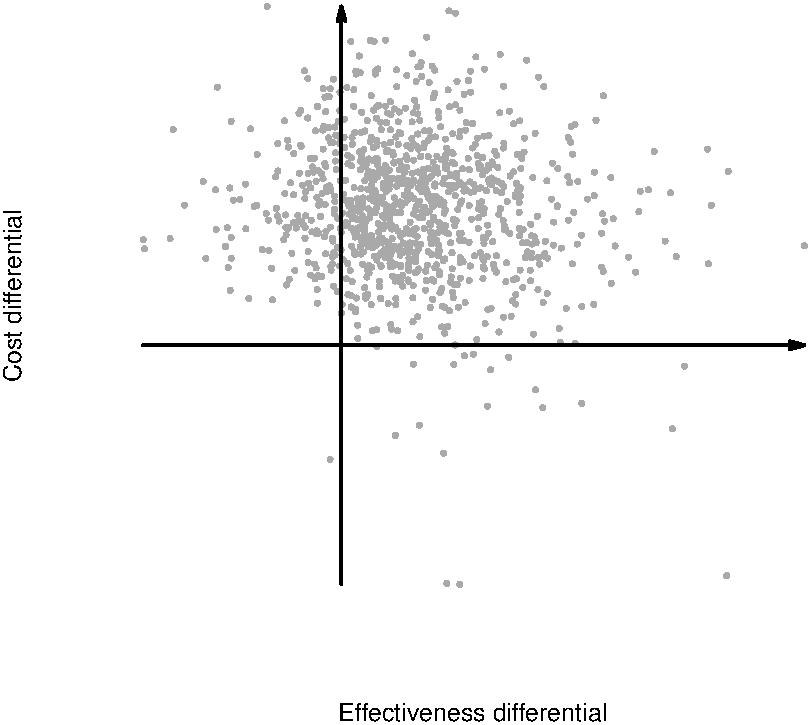
\includegraphics[scale=.55]{1.introduction-to-health-economic-evaluations/figs/CEPlane_empty}};
\draw(3.5,-.1) node[align=center,rectangle,rounded corners,draw=none,text width=4.1cm](8){\fontsize{8}{8}\selectfont $\Delta_e$};
\draw(-.9,3.2) node[align=center,rectangle,rounded corners,draw=none,text width=4.1cm](8){\fontsize{8}{8}\selectfont $\Delta_c$};
\draw(-4.0,-2.6) node[align=left,rectangle,rounded corners,draw=none,text width=4.1cm](8){\fontsize{7}{8}\selectfont $^*$Induced by $\myblue p(\bm\theta\mid \mbox{data})$};
}

\only<1-2|handout:1-2>{
\draw(4.5,3.5) node[align=center,rectangle,rounded corners,draw=none,text width=4.1cm](8){\fontsize{7}{8}\selectfont $\myblue \Delta_e=\red\underbrace{\myblue\mbox{E}[e \mid \bm{\theta}_1]}_{\mu_{e1}} \myblue - \red\underbrace{\myblue\mbox{E}[e \mid \bm{\theta}_0]}_{\mu_{e0}}$};
\draw(4.5,2.6) node[align=center,rectangle,rounded corners,draw=none,text width=4.1cm](8){\fontsize{7}{8}\selectfont $\myblue \Delta_c=\red\underbrace{\myblue\mbox{E}[c \mid \bm{\theta}_1]}_{\mu_{c1}} \myblue - \red\underbrace{\myblue\mbox{E}[c \mid \bm{\theta}_0]}_{\mu_{c0}}$};
}

\only<2|handout:2>{
\node{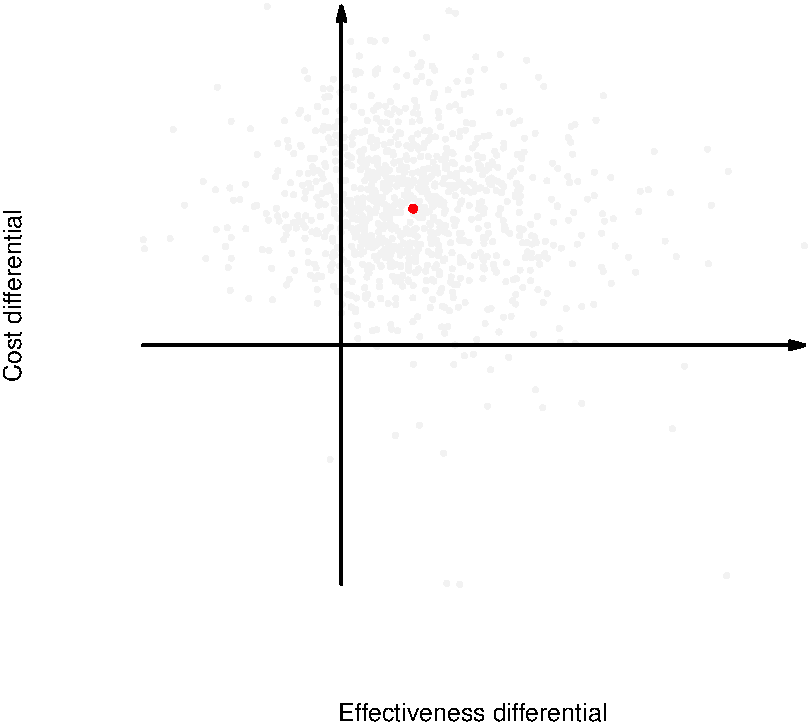
\includegraphics[scale=.55]{1.introduction-to-health-economic-evaluations/figs/CEPlane_ICER}};
\draw(3.5,-.1) node[align=center,rectangle,rounded corners,draw=none,text width=4.1cm](8){\fontsize{8}{8}\selectfont $\Delta_e$};
\draw(-.9,3.2) node[align=center,rectangle,rounded corners,draw=none,text width=4.1cm](8){\fontsize{8}{8}\selectfont $\Delta_c$};
\draw(2.3,1.5) node[align=center,rectangle,rounded corners,draw=none,text width=6.0cm](8){\fontsize{8}{8}\selectfont
\begin{eqnarray*}
\mbox{ICER}&\!\!\!\!=\!\!\!\!&\frac{\mbox{E$[\Delta_c]$}}{\mbox{E$[\Delta_e]$}}=\frac{\mbox{E}[\mu_{c1}]-\mbox{E}[\mu_{c0}]}{\mbox{E}[\mu_{e1}]-\mbox{E}[\mu_{e0}]} \\
&\!\!\!\!=\!\!\!\!&\mbox{Cost per outcome}
\end{eqnarray*}
};
}
\end{tikzpicture}
\end{overprint}
\end{figure}
}

\frame{
\frametitle{Decision-making based on the ICER}
\begin{overlayarea}{\textwidth}{1.5\textheight}
\begin{itemize}
\only<1|handout:1>{
\item ICER is not an ordered statistic
\begin{itemize}
\item {\color{blue}{-200/200}} better than {\color{red}{-100/200}} better than {\color{magenta}{-100/100}} in terms of decision, but ratios are -1, -1/2, -1
\item {\color{green!60!black!80} ICERs in the NW quadrant} indicate an intervention that is \textbf{dominated} (+ costs/- effectiveness)
\end{itemize}
}
\only<2|handout:2>{
\item Equivalent ICERs can mean very different things!
\begin{itemize}
\item $\color{red}(\mbox{E}[\Delta_e],\mbox{E}[\Delta_c])=(0.0005,5)$, indicates that the new treatment produces on average an increase in effectiveness of 0.0005 units at the cost of extra \pounds 10\,000
\item $\color{red!20!blue!80}(\mbox{E}[\Delta_e],\mbox{E}[\Delta_c])=(-0.0005,-5)$: new intervention less effective, but cheaper
\item In both cases, ICER = \pounds 10\,000
\end{itemize}
}
\end{itemize}
\centering
\only<1|handout:1>{
\vspace{-1.5cm}
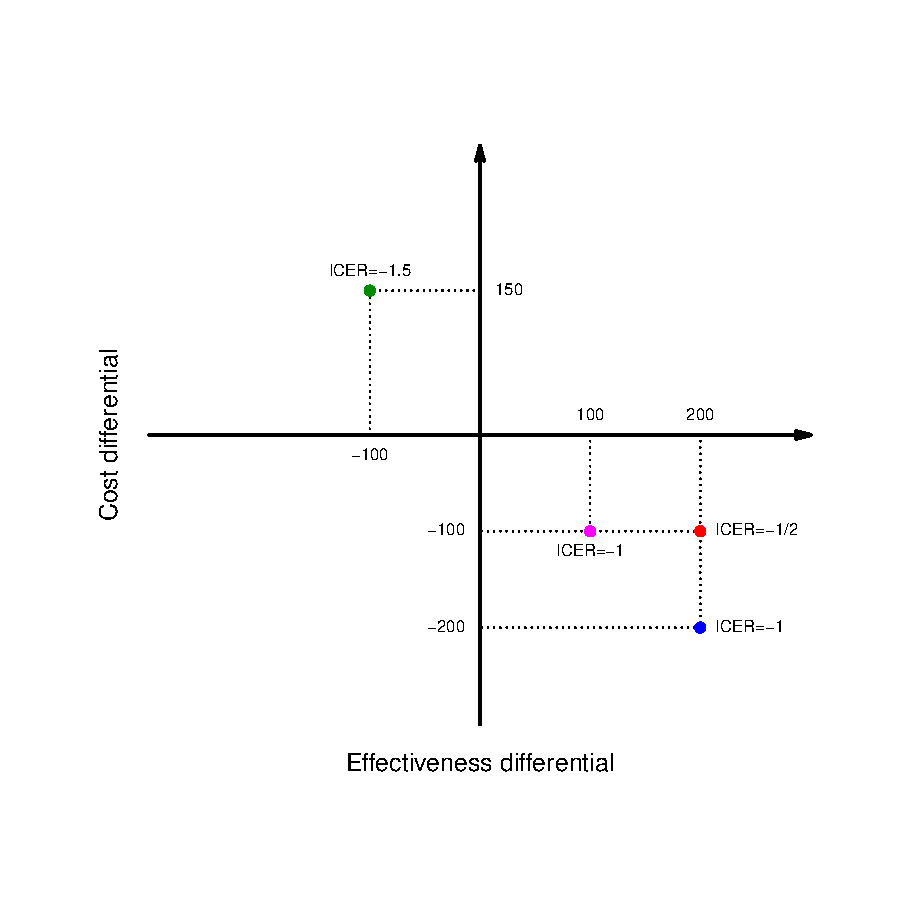
\includegraphics[scale=.56]{1.introduction-to-health-economic-evaluations/figs/ICER_not_ordered2}
}
\only<2|handout:2>{
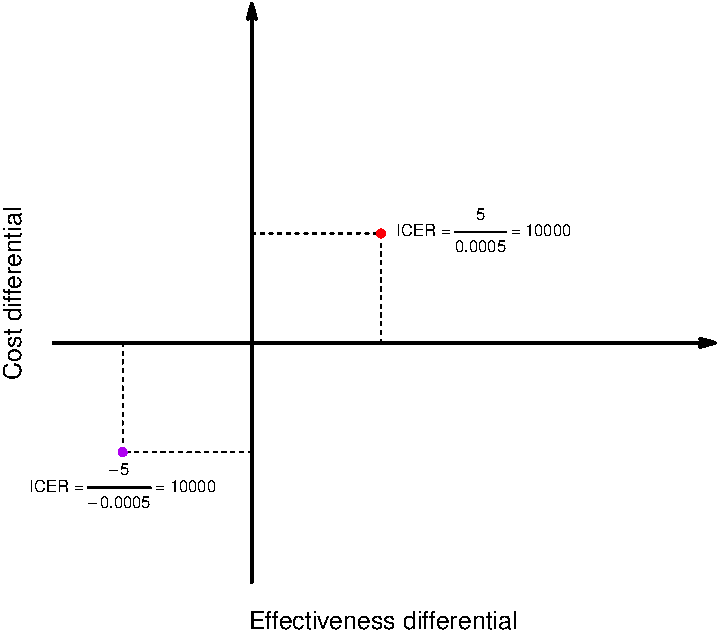
\includegraphics[scale=.54]{1.introduction-to-health-economic-evaluations/figs/ICER_not_int4}
}
\end{overlayarea}
}

\begin{frame}[label=decision_making]
\frametitle{Decision-theoretic approach to HTA}
\TabPositions{5.0cm}
\begin{itemize}
\item Analytic framework for decision-making in the face of uncertainty
\item Considers a set of \alert{prescriptive} axioms to ensure \textbf{rationality} in decision-making
\item Identifies the best course of action given:
\begin{itemize}
\item \alert{Model specification}
\item \alert{Current evidence}
\end{itemize}
\end{itemize}
\pause
\textbf{Process of rational decision-making}
\begin{tabular}{m{.7\textwidth}m{.3\textwidth}}
\begin{enumerate}
\item Describe uncertainty on \textit{all} unknown quantities by means of a (possibly subjective) \alert{probability distribution}
\end{enumerate}
& 
\vspace{-10pt}$\displaystyle\myblue p(\bm\omega)=p(e,c\mid\bm\theta)p(\bm\theta)$ \\[-13pt]
\begin{enumerate}\setcounter{enumi}{1}
\item For each intervention $t$, outcomes $o=(e,c)$ are valued by means of a pre-specified \alert{measure of utility}
\end{enumerate}
& 
\vspace{-10pt}$\displaystyle\myblue u(e,c;t)$ \\[-13pt]
\begin{enumerate}\setcounter{enumi}{2}
\item Select as the most ``cost-effective'' the intervention that is associated with the \alert{maximum expected utility}
\end{enumerate}
& 
\vspace{-10pt}$\displaystyle\myblue \mathcal{U}^t=\mbox{E}_{\bm\omega}[u(e,c;t)]$
\end{tabular}
\pause
\begin{itemize}
\item Typical utility function in HTA: \alert{Monetary Net Benefit} \hfill $\displaystyle\myblue u(e,c;t) = nb_t = ke_t-c_t$
\begin{itemize}
\item $k$ is the ``willingness to pay'', i.e.\ the \textit{\red cost per extra unit of effectiveness gained}
\item Fixed, \alert{linear} form, which simplifies computations
\item Assumes decision-maker is \textit{risk neutral}. Not necessarily true!
\end{itemize}
\end{itemize}
\end{frame}

\begin{frame}[label={EIB_def}]
\frametitle{ICER vs EIB}
\begin{itemize}
\item Under the MNB, the expected utility is \myblue
\begin{eqnarray*} 
\mathcal{U}^t = \mathcal{NB}_t &\!\!\!\!\!=\!\!\!\!\!& \mbox{E}{\color{blue}_{\bm\omega}}[u(e,c;t)] \\
&\!\!\!\!\!=\!\!\!\!\!& k\mbox{E}{\color{blue}_{\bm\omega}}[e_t] - \mbox{E}{\color{blue}_{\bm\omega}}[c_t] \\
&\!\!\!\!\!=\!\!\!\!\!& k\mbox{E}{\color{red}_{\bm\theta}}[e\mid \bm\theta_t]-\mbox{E}{\color{red}_{\bm\theta}}[c\mid\bm\theta_t] =  k\mbox{E}[\mu_{et}]-\mbox{E}[\mu_{ct}]
\end{eqnarray*}\black 
\textbf{NB}: The expectation is taken with respect to $p(\bm\omega)$ so $\mathcal{NB}_t$ is a pure number!

\vspace{10pt}\pause
\item Assuming we are considering only two interventions $t=(0,1)$, decision-making can be effected by looking at the \alert{Expected Incremental Benefit} \myblue
\begin{eqnarray*}
\mbox{EIB} & = & \mathcal{NB}_1-\mathcal{NB}_0 \\
& = & \left(k\mbox{E}[\mu_{e1}]-\mbox{E}[\mu_{c1}]\right) - \left(k\mbox{E}[\mu_{e0}]-\mbox{E}[\mu_{c0}]\right)\\
&=& k\mbox{E}[\Delta_e] - \mbox{E}[\Delta_c]
\end{eqnarray*}\black 

\pause\vspace{-5pt}
\item The reference treatment $t=1$ is more cost-effective than the comparator $t=0$ if \myblue
\begin{eqnarray*}
\mbox{EIB}>0 \Rightarrow k>(<)\frac{\mbox{E}[\Delta_c]}{\mbox{E}[\Delta_e]} = \mbox{ICER} \quad \mbox{if $\mbox{E}[\Delta_e]>(<)0$}
\end{eqnarray*}
\end{itemize}
\end{frame}

\frame{
\frametitle{\only<1-2|handout:1-2>{Cost-effectiveness plane vs EIB vs ICER}\only<3|handout:3>{EIB vs Willingness to pay $k$}\only<4|handout:4>{Cost effectiveness acceptability curve}}
\begin{center}
\only<1|handout:1>{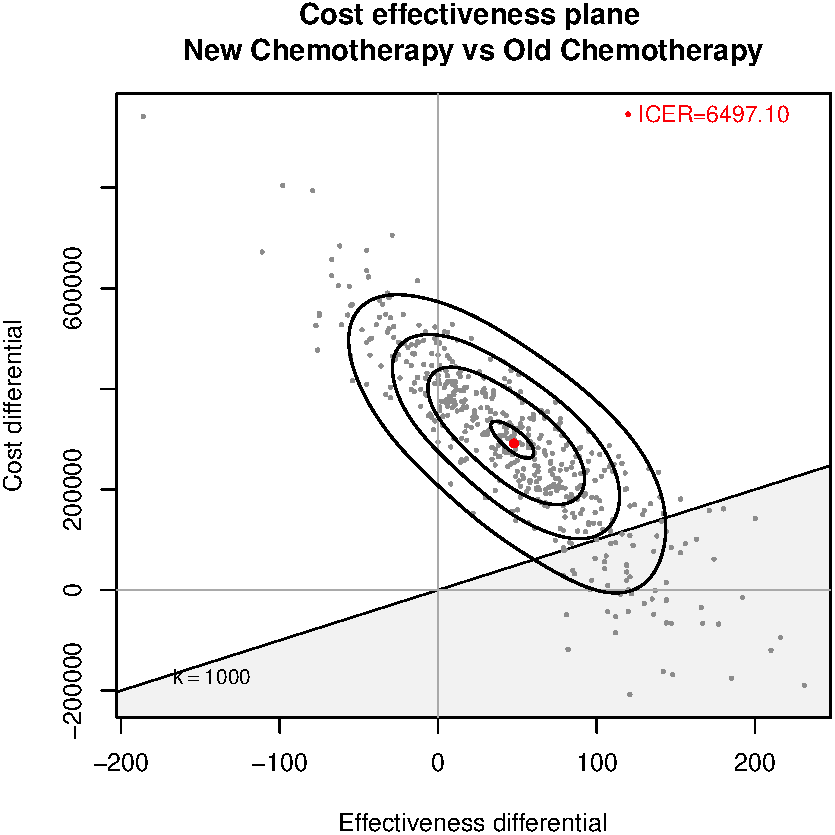
\includegraphics[width=7.6cm]{5.statistical-cost-effectiveness-analysis/figs/contour2_2}}
\only<2|handout:2>{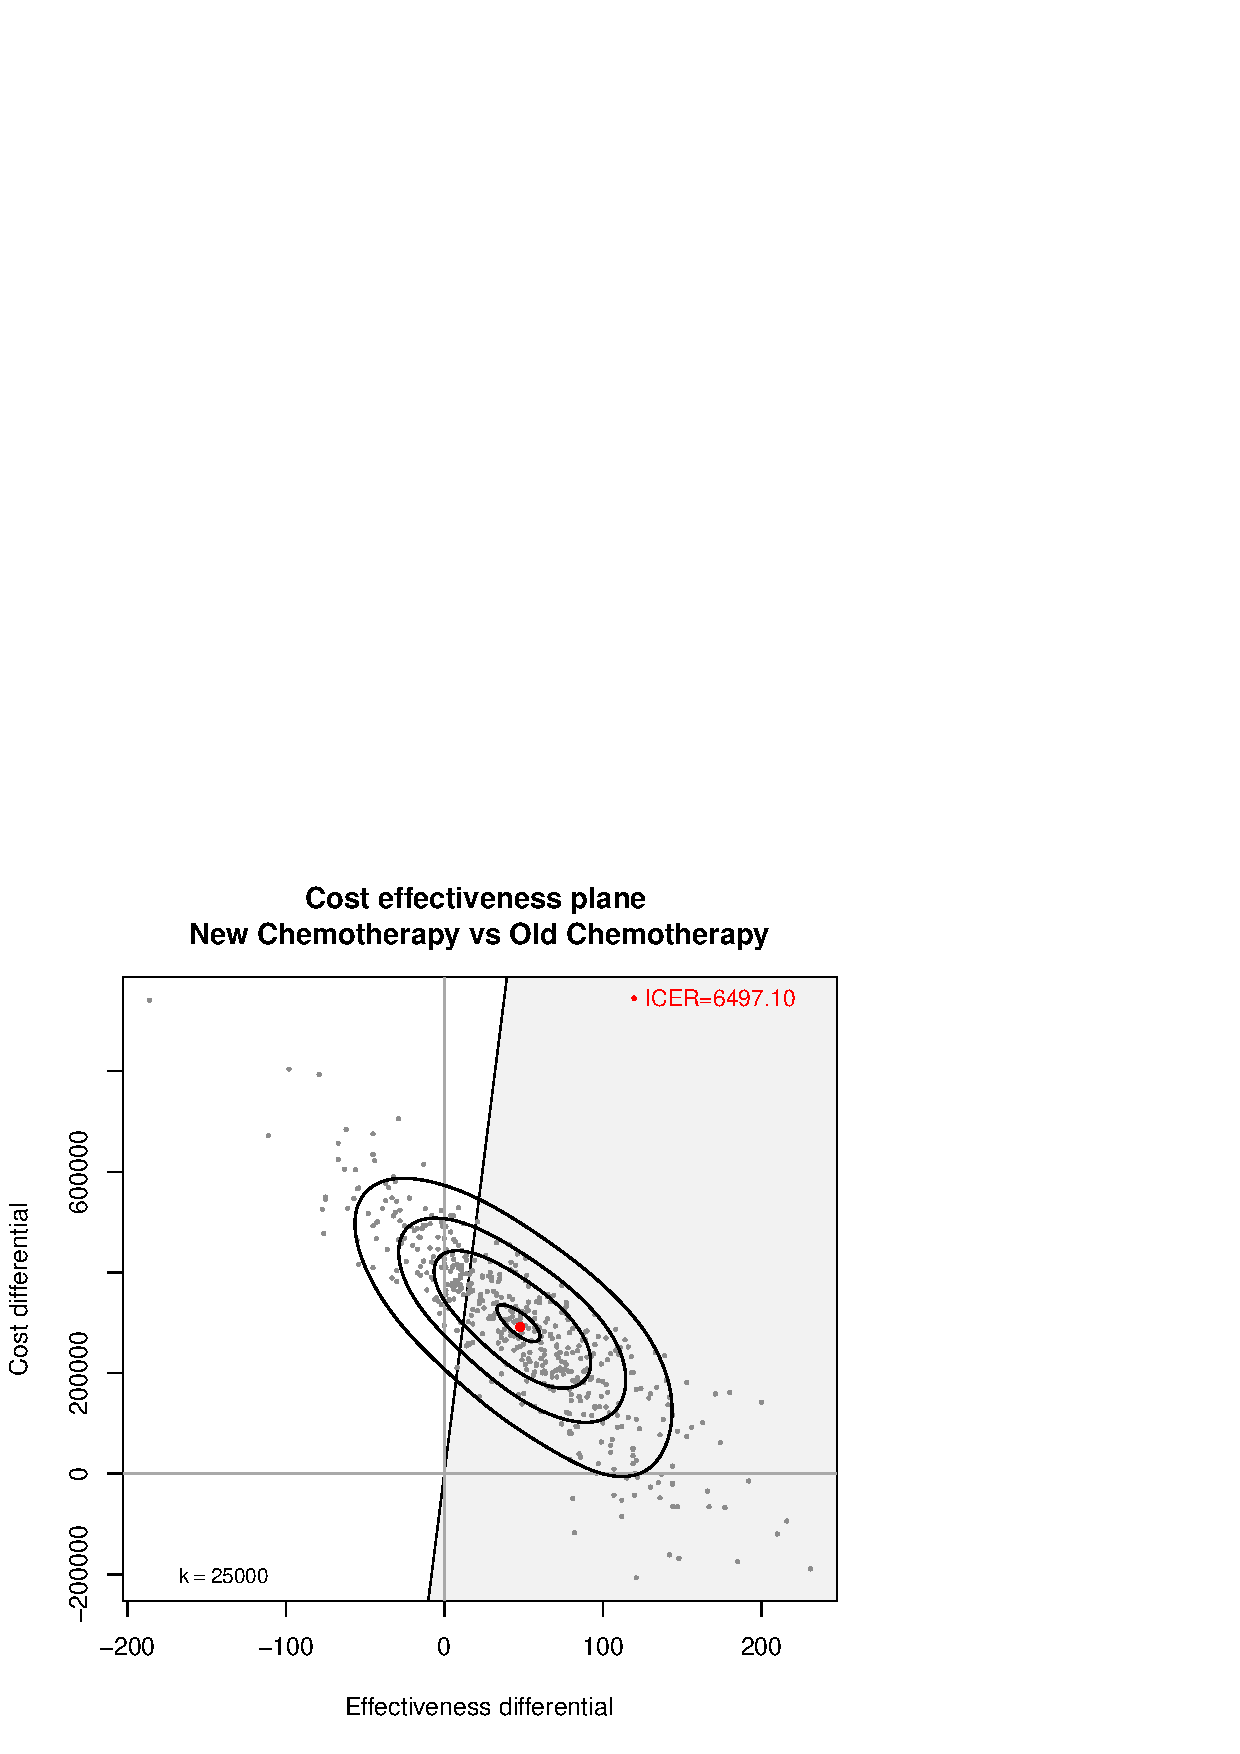
\includegraphics[width=7.6cm]{5.statistical-cost-effectiveness-analysis/figs/contour2}}
\only<3|handout:3>{\rotatebox{0}{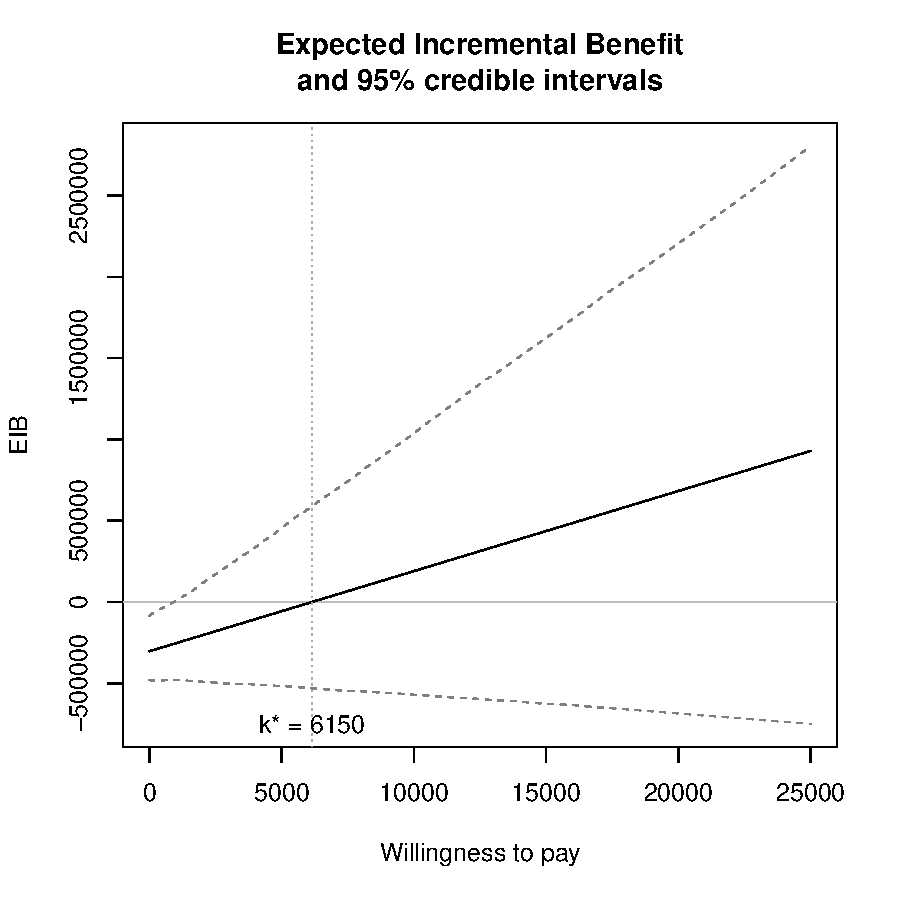
\includegraphics[scale=.53]{1.introduction-to-health-economic-evaluations/figs/chemo_INB}}}
\only<4|handout:4>{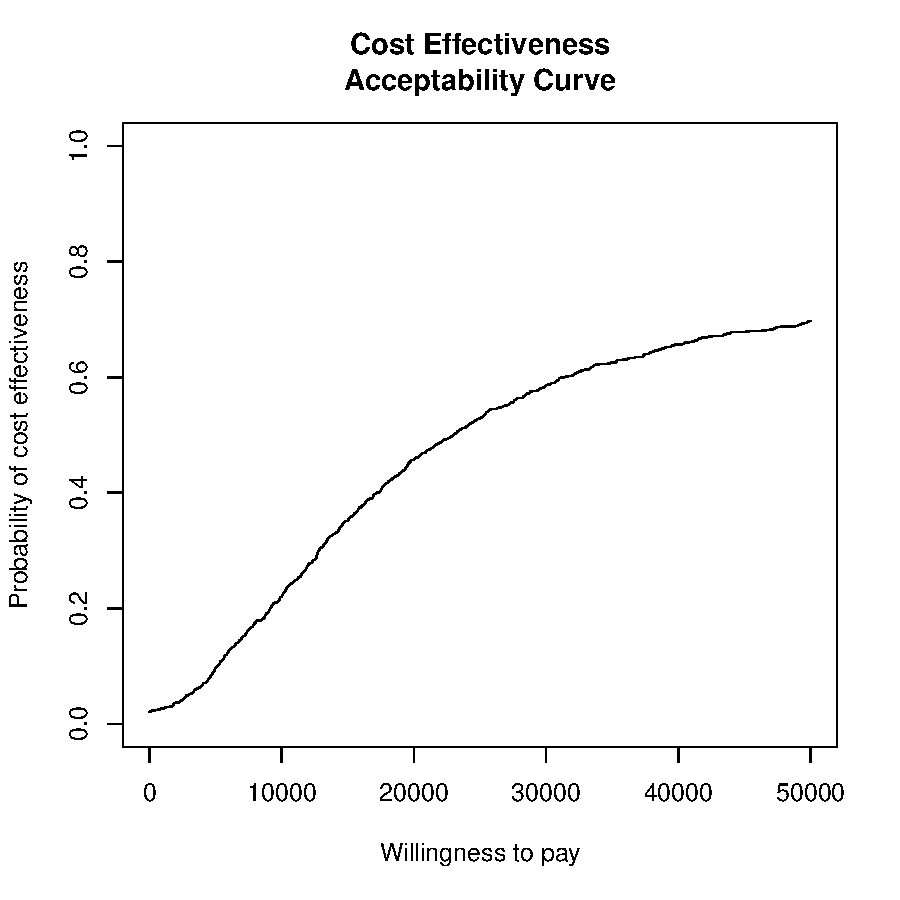
\includegraphics[width=7.6cm]{6.probabilistic-sensitivity-analysis/figs/CEAC}}
\end{center}
}

 \nologo
%
%\part{Decision trees}\label{dectrees} \frame{\partpage} \UCL
%\begin{frame}

\frametitle{Model-based economic evaluation}

\bi

\item Trial-based economic evaluation
  \begin{itemize}
  \item assess cost-effectiveness based on individual-level data on
    costs and effects
  \item shorter-term, selected population
  \end{itemize}

\item Model-based economic evaluation
  \begin{itemize}
  \item construct a model-based representation of disease/clinical
    history
  \item State-transition (usually \emph{Markov}) models for clinical
  histories very common
  \item ``populate'' model with available + relevant data.
  \end{itemize}

\item Model-based evaluation typically used to estimate
  \begin{itemize}
  \item \alert{long-term} cost-effectiveness
  \item in wider population 
  \end{itemize}
  by combining data from trials with other sources of evidence.

\ei

\vfill 
\begin{block}{\footnotesize References}
\bmhe,  chapter 5.4.\\
\esdmh
\end{block}
\end{frame}

%### New page ############################################################

\frame{%
\frametitle{Summary}
\begin{itemize}
\item Decision tree model
\begin{itemize}
\item Strengths and limitations
\item When to use and when not use
\end{itemize}
\item How to calculate on a decision tree
\begin{itemize}
\item `Forward' method
\item `Backward' method
\end{itemize}
\item Examples
\end{itemize}

\vfill
\begin{block}{\footnotesize References}
Decision Making in Health and Medicine, Weinstein et al, Cambridge University Press
\end{block}

}


\begin{frame}
\frametitle{Steps in constructing and analysing Decision Trees}
A decision tree is a visual representation of a decision analysis:
	\begin{itemize}
		\item \alert{Structure} the tree
		\pause
		\item Estimate \alert{probabilities}
		\pause
		\item Estimate \alert{payoffs} (assign values to costs and outcomes)
		\pause
		\item Analyse the tree
		\pause
			\begin{itemize}
				\item \alert{Evaluate} the tree
				\item Explore \alert{uncertainty}
			\end{itemize}
	\end{itemize}
\end{frame}

\begin{frame}
\frametitle{Structuring the Decision Tree}
A decision tree is made up of nodes, branches and outcomes

\begin{itemize}
	\item Nodes:
	\begin{itemize}
		\pause
		\item \textcolor{blue}{Decision node (square)}: Describes the problem. Deterministic choice.
		\pause
		\item \textcolor{green}{Chance node (circle)}: Represents the point at which several possible events can occur.
		\pause
		\item \textcolor{red}{Terminal node (triangle)}: Represents the end of a tree with a payoff attached.
	\end{itemize}
\end{itemize}
\end{frame}

\begin{frame}
A hypothetical example is of a comparison between two drugs, `Drug A' and
`Drug B'. Each drug has different costs associated with them and
different performance in terms of the chance that the drug is successful at treating the patient.

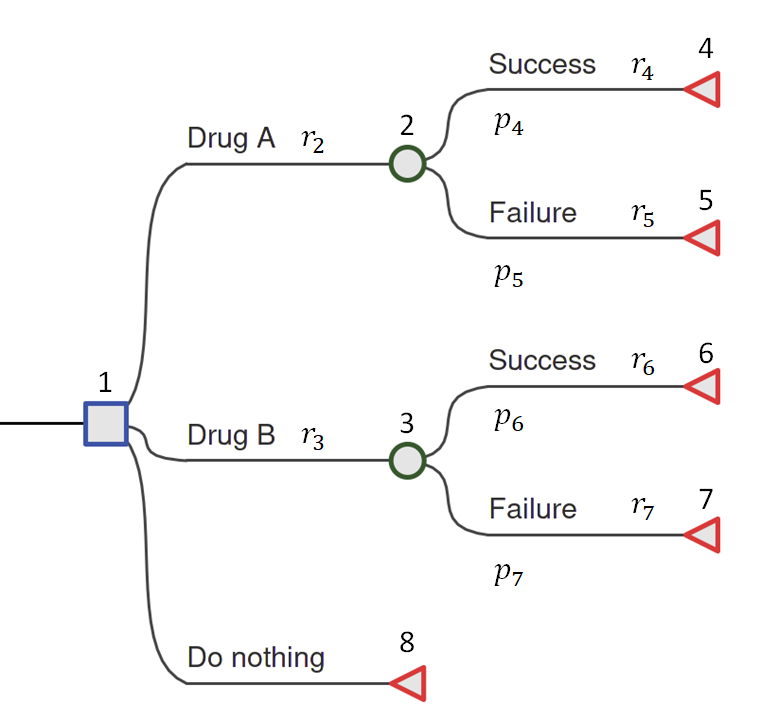
\includegraphics[width=\textwidth,height=0.8\textheight, keepaspectratio]{decision-trees/figs/dectree.png}

\end{frame}

\begin{frame}
\frametitle{Structuring the Decision Tree}
	\begin{itemize}
		\item Branches issuing from a chance node represent possible events patients may experience at that point in the tree.
		\item Branch probabilities represent the likelihood of each event.
		\item The sequence of chance nodes from left to right usually follows the sequence of events.
		\item The events stemming from a chance node must be \alert{mutually exclusive} and probabilities should sum to 1.
	\end{itemize}
\end{frame}


\begin{frame}
\frametitle{Advantages of Decision Trees}

	\begin{itemize}
		\item They enable the economic question to be structured in a \alert{meaningful} and \alert{visual} manner.
		\pause
		\item  They allow data informing the model parameters to be assimilated and, where appropriate, synthesised.
		\pause
		\item They are relatively simple to undertake and suitable for:
		\begin{itemize}
			\item Diseases that occur only once.
			\item Decisions about acute care.
			\item Decisions with short time frames.
		\end{itemize}
	\end{itemize}
\end{frame}


\begin{frame}
\frametitle{Limitations of Decision Trees}

	\begin{itemize}
		\item They do not explicitly account for passage of time:
			\begin{itemize}
				\item Passage of time accounted for by outcome measure.
				\item Limited ability to account for long term outcomes.
			\end{itemize}
			\pause
		\item Possible to add branches but results in a complex model.
		\item Other modelling techniques can handle repeated events better.
		\item Structure of tree only allows for one-way progression of patient through model: Not movement back and forth between states.
		\item Decision trees can still be useful as a sub-model.
		\end{itemize}
\end{frame}


\begin{frame}
\frametitle{}
 
\includegraphics[width=1\textwidth,height=1.2\textheight, keepaspectratio]{decision-trees/figs/nice-guidance}
\end{frame} 

\begin{frame}
\frametitle{Simple decision tree example: New TST guidelines}
 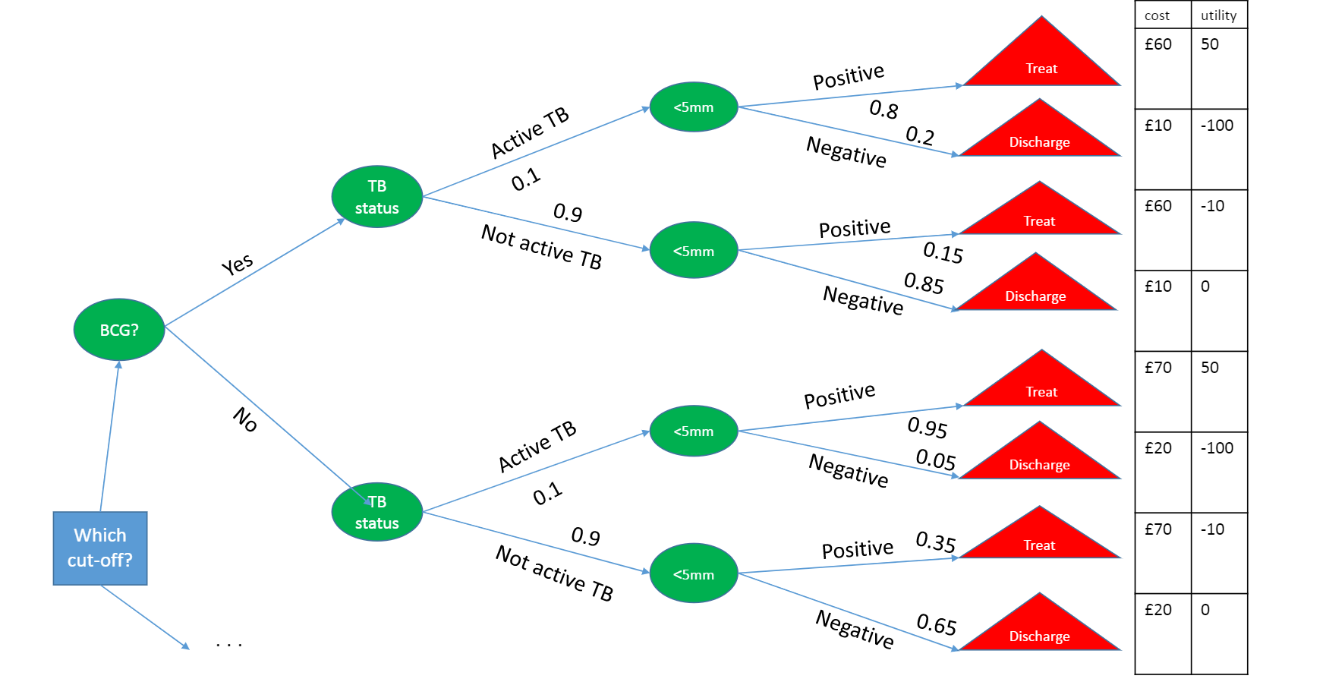
\includegraphics[width=\textwidth,height=0.8\textheight, keepaspectratio]{decision-trees/figs/tb-decision-tree}
\end{frame}


\begin{frame}
\frametitle{Calculations on a decision tree}

\begin{itemize}
 \item Conditional probabilities two or more events 
 \item Probability of both A and B occurring, divided by the probability of B occurring
 \item The joint probability of A and B measures the probability that A and B occur together at the same moment.
 \item The marginal probability of A is the individual probability of A, ignoring any value of event B.
\end{itemize}

\end{frame}

\begin{frame}
\frametitle{Probabilities of moving along branches}

\begin{itemize}
 \item Complete set of all possible outcomes is set of terminal nodes on the RHS
\pause
 \item By chaining the conditional probabilities for a given pathway we obtain the total or
\emph{joint} probability of reaching a terminal node. Each pathway
through the tree is a mutually exclusive sequence of events. Consider
one such pathway through the tree with the following \(n\) nodes.

\[
x_0 \rightarrow x_{[1]} \rightarrow x_{[2]} \rightarrow \cdots \rightarrow x_{[n]}
\]
where 
\begin{itemize}
\item \(x_0\) is the root node (often the decision node)
\item \(x_{[n]}\) is the terminal node and the square brackets indicate that this is the \(ith\) ordered nodes in the sequence.
\end{itemize}
\pause
 \item By the product rule joint probability of this path is

\[
p(x_{[1]}, x_{[2]}, \ldots, x_{[n]}) =
p(x_{[2]} \mid x_{[1]}) p(x_{[3]} \mid x_{[2]}) \cdots  p(x_{[n]} \mid x_{[n - 1]}) =
\]
\[
\prod_i^{[n - 1]} p(x_{[i + 1]} \mid x_{[i]})
\]
\pause
 \item For the above pathway, the corresponding cost and effects are
\(c_{[1]}, c_{[2]}, \ldots, c_{[n]}\) and
\(e_{[1]}, e_{[2]}, \ldots, e_{[n]}\).
\end{itemize}

\end{frame}

\begin{frame}
\frametitle{How to calculate expected values}

There are two alternative approaches used for calculating the expected
cost and effectiveness on a decision tree.

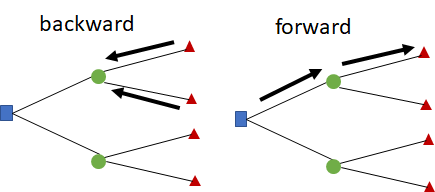
\includegraphics{decision-trees/figs/forward-backward-diagram.png}

\end{frame}

\begin{frame}
\frametitle{"Backward" computation}

\begin{itemize}
 \item Weighted average of the total values of the child nodes of a parent chance node
 \begin{itemize}
  \item Weights are the probability of traversing each branch to the child nodes.
 \end{itemize}
\pause
 \item Act of stepping backwards in this way through the tree is called \emph{folding back} (or \emph{rolling back}).
\pause
 \item So called because the children are folded up or collapsed, so that the chance node is now represented by its expected value.
\pause
 \item Starting at the right-most terminal nodes the expected values at each chance node are calculate in turn and the tree can thus be folded back all the way to the decision node
\pause
 \item Example of something called a \emph{recursive} function which is a function that calls itself during its execution.
 \begin{itemize}
  \item A well-known example is when calculating the Fibonacci series.
  \end{itemize}
 \item This approach is part of a whole field of stochastic optimisation in applied probability called Markov decision process (MDP).
 \end{itemize}

\end{frame}

\begin{frame}
\frametitle{"Backward" computation}

\begin{itemize}
 \item Recall the conditional probabilities \(p_{ij} = p(x_j \mid x_i)\), then
the expected value is

\[
\mathbb{E}[V_i] =   \left\{
    \begin{array}{lcl}
      r_i & \mbox{ if } & i \in \mathcal{S}_{term}\\
      r_i + \sum p_{ij} \mathbb{E}[V_j] & & \mbox{otherwise}
    \end{array}
  \right.
\]
where
\begin{itemize}
\item \(\mathbb{E}\) is the weighted average of the values, \(V\) is the random variable total node value, e.g.~cost or QALYs
 \item \(r_i\) is the (unit) value at node \(i\)
 \item \(\mathcal{S}_{term}\) is the set of all terminal nodes. Note that at a terminal node the expected value is simply the value at that node.
\pause
 \end{itemize}
 \item An advantage of using this method is that total expected values can be obtained at each node and so if there are multiple decision node not at the root of the tree the recursive approach can fold-back sub-trees.
\end{itemize}

\end{frame}

\begin{frame}
\frametitle{Simple decision tree example: New TST guidelines}
 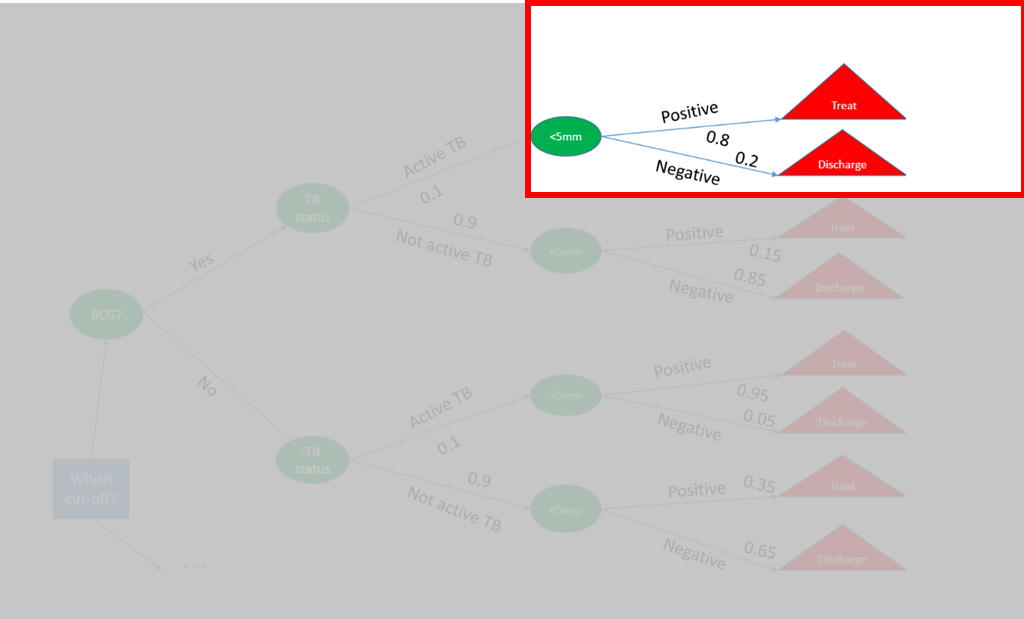
\includegraphics[width=\textwidth,height=0.8\textheight, keepaspectratio]{decision-trees/figs/folding-back1}
\end{frame}

\begin{frame}
\frametitle{Simple decision tree example: New TST guidelines}
 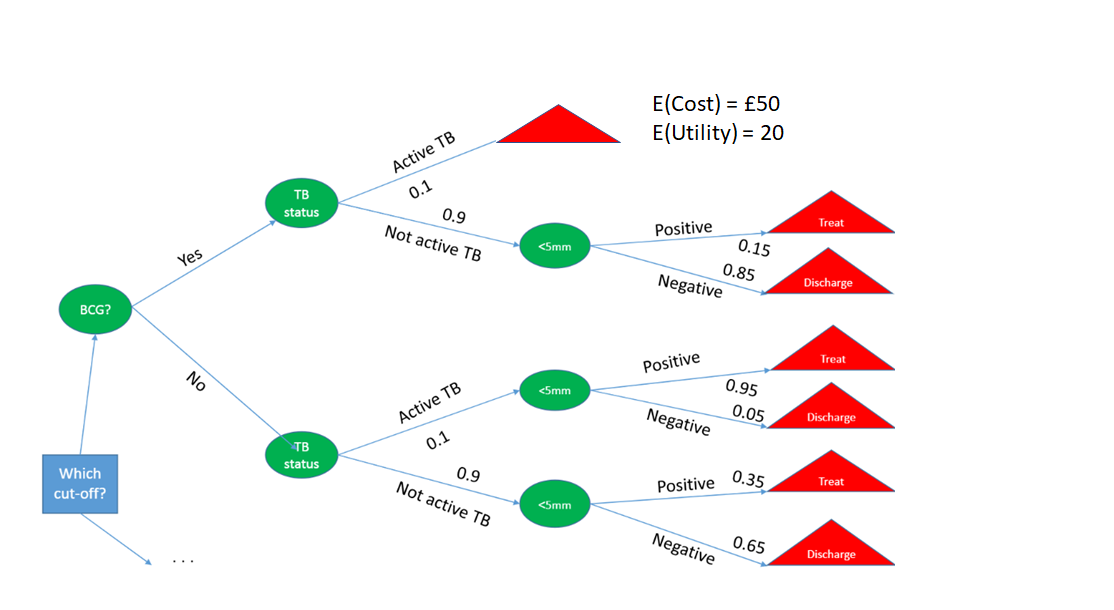
\includegraphics[width=\textwidth,height=0.8\textheight, keepaspectratio]{decision-trees/figs/folding-back2}
\end{frame}

\begin{frame}
\frametitle{Simple decision tree example: New TST guidelines}
 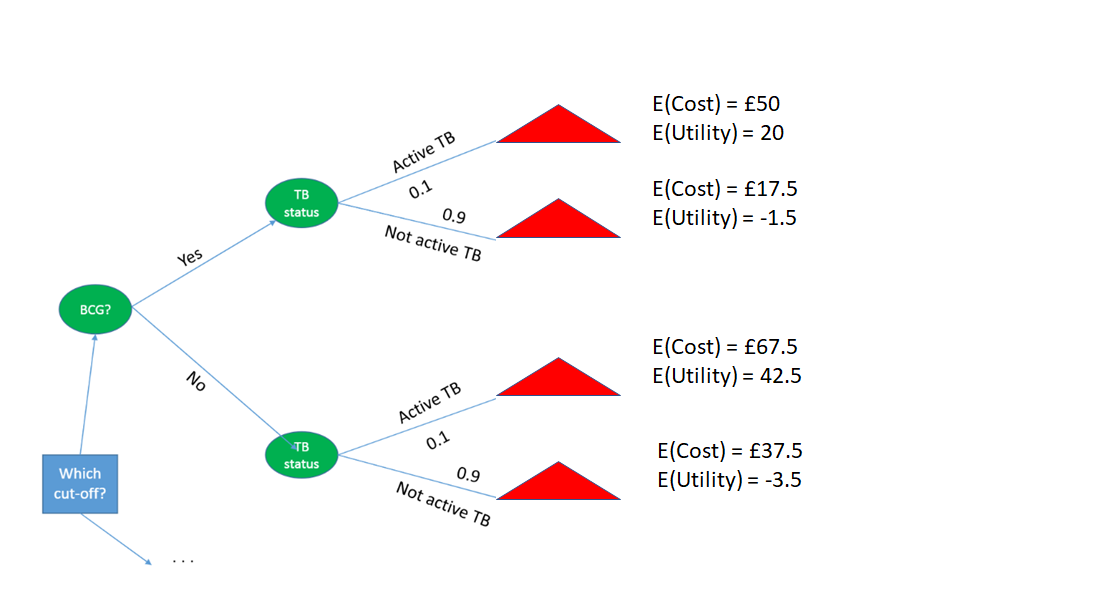
\includegraphics[width=\textwidth,height=0.8\textheight, keepaspectratio]{decision-trees/figs/folding-back3}
\end{frame}

\begin{frame}
\frametitle{Simple decision tree example: New TST guidelines}
 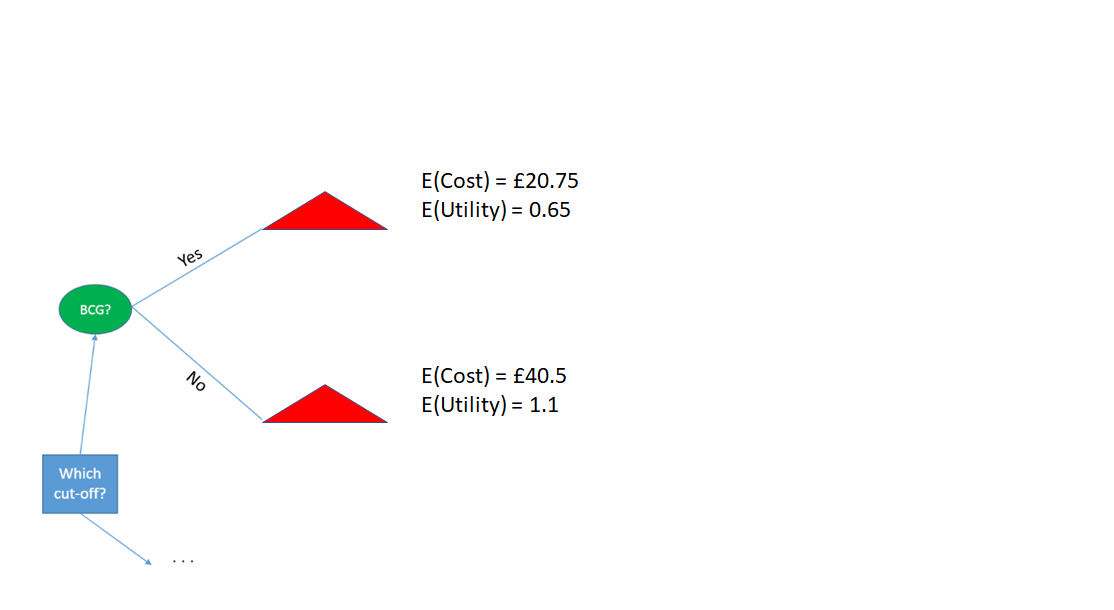
\includegraphics[width=\textwidth,height=0.8\textheight, keepaspectratio]{decision-trees/figs/folding-back4}
\end{frame}


\begin{frame}
\frametitle{"Forward" computation}

 \begin{itemize}
 \item May be more intuitive
\pause
 \item Calculate the total health and costs, and joint probability along all of the distinct pathways of the tree corresponding to a decision.
\pause
 \item The weighted average of the costs or health values give the expected value at the decision node.
\pause

\item Formally

\[
\mathbb{E}[V] = \sum_{j \in S_{term}} r^*_j p^*_j
\]
where

 \begin{itemize}
 \item \(r^*_j = r_{[1]} + r_{[2]} + \cdots + r_{[n]}\) is the total of the values along each pathway with terminal node \(j\)
 \item \(p^*_j = p(x_{[1]}, x_{[2]}, \ldots, x_{[n]})\) is the joint probabilities of traversing the unique path with terminal node \(j\).
 \item The set of possible terminal nodes if the decision-maker takes a given decision is denoted \(S_{term}.\)
 \end{itemize}
\end{itemize}

\end{frame}


\begin{frame}
\frametitle{TB Combined probabilities for each branch}
 If probability of BCG is $0.1$ (c.f. NHS Immunisation Statistics, England 2012-13) then
\begin{eqnarray*}
p^*_1 &=& 0.1 \times 0.1 \times 0.8 = 0.008\\
p^*_2 &=& 0.1 \times 0.1 \times 0.2 = 0.002\\
p^*_3 &=& 0.1 \times 0.9 \times 0.15 = 0.0135\\
p^*_4 &=& 0.1 \times 0.9 \times 0.85 = 0.0765\\
p^*_5 &=& 0.9 \times 0.1 \times 0.95 = 0.0855\\
p^*_6 &=& 0.9 \times 0.1 \times 0.05 = 0.0045\\
p^*_7 &=& 0.9 \times 0.9 \times 0.35 = 0.2835\\
p^*_8 &=& 0.9 \times 0.9 \times 0.65 = 0.5265
\end{eqnarray*}
\end{frame}

\begin{frame}
\frametitle{TB expected cost and health impact}

Cost:

\begin{eqnarray*}
&& 0.008 \times 60 + 0.003 \times 10 + 0.0135 \times 60 + 0.0765 \times 10\\
&& + 0.0855 \times 70 + 0.0045 \times 20 + 0.2835 \times 70 + 0.5265 \times 20\\
&& = 38.535
\end{eqnarray*}

Health:

\begin{eqnarray*}
&& 0.008 \times 50 + 0.003 \times (-100) + 0.0135 \times (-10) + 0.0765 \times 0\\
&&  + 0.0855 \times 50 + 0.0045 \times (-100) + 0.2835 \times (-10) + 0.5265 \times 0\\
&& = 0.955
\end{eqnarray*}

\end{frame}



 \nologo
%
%\part{Markov models}\label{MM} \frame{\partpage} \UCL
%
\begin{frame}
  
\frametitle{Outline of this lecture} 

\begin{itemize}

\item Theory of Markov modelling

\item Example: Estimating Markov model transition probabilities from
  individual-level counts of transitions

\item Bayesian inference ideas
  \begin{itemize}
  \item Dirichlet and Multinomial distributions
  \item Advantages of Bayes: including prior information, natural
    quantification of uncertainty (probabilistic sensitivity
    analysis).
  \end{itemize}

\item Implementing Markov models in \texttt{R}

\item Brief discussion of decision modelling more generally, from
  Bayesian perspective
\end{itemize}


\end{frame}


%### New page ############################################################



\frame{
  \frametitle{Markov models in discrete time}

  Assume 
  \begin{itemize}

  \item a set of $S$ ``clinically relevant'' states: exhaustive and mutually exclusive

  \item a discrete time axis, indexed by ``cycles'' or time units $j$

  \item a set of allowed transitions in a diagram of the states
  \end{itemize} 
  
  Arrows connecting two states denote that a person can move
  \begin{itemize}
  \item  from the state at the start of the arrow at time $j$ 
  \item  to the state at the end of the arrow at time $j+1$
  \item Absence of an arrow implies transition is not allowed by model
  \end{itemize}


  \pause
Movements occur according to suitable \alert{\textit{transition probabilities}}
\[ \myblue \bm{\pi}_j = \bm{\pi}_{j-1}\bm\Lambda_j \]
\begin{itemize}
\item $\myblue \bm{\pi}_j$ is the vector of probabilities of occupying each state at time $j$
\item $\myblue \bm\Lambda_j = [\Lambda_{j;s,s'}]$ is the \alert{transition probability matrix} at time $j$: $s,s'$ entry is the probability of moving from state $s$ to state $s'$ at time $j$
\end{itemize}

}

\frame{
\frametitle{Markov models}
\only<1|handout:1>{1.\ Define a structure}
\only<2|handout:2>{2.\ Estimate the transition probabilities from available, relevant data\\Define costs and utilities associated with occupying each state $s$ at each time $j$}
\only<3|handout:3>{3.\ Run the simulation, recording:\\ proportion of people in each state $\rightarrow$ expected costs and effects,\\ at each time:\\ $j=0$}
\only<4|handout:4>{3.\ Run the simulation: $j=1$}
\only<5|handout:5>{3.\ Run the simulation: $j=2$}
\only<6|handout:6>{3.\ Run the simulation: $j=3$}
\only<7|handout:7>{3.\ Run the simulation: $j=J$}
\begin{figure}
\begin{tikzpicture}
\draw(0,1.5) node[align=center,ellipse,draw,fill=none,font=\sffamily\fontsize{9}{10}\selectfont,minimum width=1.8cm,minimum height=.7cm](1){Disease};

\draw(-2.5,0) node[align=center,ellipse,draw,fill=none,font=\sffamily\fontsize{9}{10}\selectfont,minimum width=1.8cm,minimum height=.7cm](2){In health};

\draw(2.5,0) node[align=center,ellipse,draw,fill=none,font=\sffamily\fontsize{9}{10}\selectfont,minimum width=1.8cm,minimum height=.7cm](3){Death};

\draw(0,-1.5) node[align=center,ellipse,draw,fill=none,font=\sffamily\fontsize{9}{10}\selectfont,minimum width=1.8cm,minimum height=.7cm](4){Recovery};

\only<2-|handout:2->{
\draw(-1.4,1.6) node[align=center,fill=none,font=\sffamily\fontsize{9}{10}\selectfont,minimum width=1.8cm,minimum height=.7cm](5){$\lambda_{22}$};

\draw(-4.0,0) node[align=center,fill=none,font=\sffamily\fontsize{9}{10}\selectfont,minimum width=1.8cm,minimum height=.7cm](6){$\lambda_{11}$};

\draw(-1.7,.9) node[align=center,fill=none,font=\sffamily\fontsize{9}{10}\selectfont,minimum width=1.8cm,minimum height=.7cm](7){$\lambda_{12}$};

\draw(1.7,.9) node[align=center,fill=none,font=\sffamily\fontsize{9}{10}\selectfont,minimum width=1.8cm,minimum height=.7cm](8){$\lambda_{24}$};

\draw(-.8,.2) node[align=center,fill=none,font=\sffamily\fontsize{9}{10}\selectfont,minimum width=1.8cm,minimum height=.7cm](9){$\lambda_{14}$};

\draw(4,0) node[align=center,fill=none,font=\sffamily\fontsize{9}{10}\selectfont,minimum width=1.8cm,minimum height=.7cm](10){$\lambda_{44}$};

\draw(.35,-.6) node[align=center,fill=none,font=\sffamily\fontsize{9}{10}\selectfont,minimum width=1.8cm,minimum height=.7cm](11){$\lambda_{23}$};

\draw(-1.7,-.8) node[align=center,fill=none,font=\sffamily\fontsize{9}{10}\selectfont,minimum width=1.8cm,minimum height=.7cm](12){$\lambda_{31}$};

\draw(1.7,-.8) node[align=center,fill=none,font=\sffamily\fontsize{9}{10}\selectfont,minimum width=1.8cm,minimum height=.7cm](13){$\lambda_{34}$};
}

\draw(-2.5,-1.7) node(box_healthy){
\begin{minipage}{0.1\textwidth}
\only<1-2|handout:1-2>{\white
\Gentsroom \Ladiesroom \Ladiesroom \Gentsroom \Gentsroom \Ladiesroom \\
\Ladiesroom \Gentsroom \Gentsroom \Ladiesroom \Ladiesroom \Gentsroom \\
\Gentsroom \Ladiesroom \Ladiesroom \Gentsroom \Gentsroom \Ladiesroom \\
\Ladiesroom \Gentsroom \Ladiesroom \Ladiesroom \Gentsroom \Gentsroom
}
\only<3|handout:3>{\blue
\Gentsroom \Ladiesroom \Ladiesroom \Gentsroom \Gentsroom \Ladiesroom \\
\Ladiesroom \Gentsroom \Gentsroom \Ladiesroom \Ladiesroom \Gentsroom \\
\Gentsroom \Ladiesroom \Ladiesroom \Gentsroom \Gentsroom \Ladiesroom \\
\Ladiesroom \Gentsroom \Ladiesroom \Ladiesroom \Gentsroom \Gentsroom
}
\only<4|handout:4>{\blue
\Gentsroom \Ladiesroom \Ladiesroom \Gentsroom \Gentsroom \Ladiesroom \\
\Ladiesroom \Gentsroom \Gentsroom \Ladiesroom \Ladiesroom \Gentsroom \\
\Gentsroom \Ladiesroom \Ladiesroom \Gentsroom \Gentsroom \Ladiesroom \\
\Gentsroom \white \Ladiesroom \Ladiesroom \Gentsroom \Ladiesroom \Gentsroom
}
\only<5|handout:5>{\blue
\Gentsroom \Ladiesroom \Ladiesroom \Gentsroom \Gentsroom \Ladiesroom \\
\Ladiesroom \Gentsroom \Gentsroom \Ladiesroom \Ladiesroom \Gentsroom \\
\Gentsroom \Ladiesroom \Ladiesroom \Gentsroom \white \Gentsroom \Ladiesroom \\
\Gentsroom \Ladiesroom \Ladiesroom \white\Gentsroom \Ladiesroom \Gentsroom
}
\only<6|handout:6>{\blue
\Gentsroom \Ladiesroom \Ladiesroom \Gentsroom \Gentsroom \Ladiesroom \\
\Ladiesroom \Gentsroom \Gentsroom \Ladiesroom \Ladiesroom \Gentsroom \\
\white \Gentsroom \Ladiesroom \Ladiesroom \Gentsroom \Gentsroom \Ladiesroom \\
\Gentsroom \Ladiesroom \Ladiesroom \white\Gentsroom \Ladiesroom \Gentsroom
}
\only<7|handout:7>{\white
\Gentsroom \Ladiesroom \Ladiesroom \Gentsroom \Gentsroom \Ladiesroom \\
\Ladiesroom \Gentsroom \Gentsroom \Ladiesroom \Ladiesroom \Gentsroom \\
\Gentsroom \Ladiesroom \Ladiesroom \Gentsroom \Gentsroom \Ladiesroom \\
\Gentsroom \Ladiesroom \Ladiesroom \Gentsroom \Ladiesroom \Gentsroom
}
\end{minipage}
};

\draw(3,-1.5) node(box_dead){
\begin{minipage}{0.1\textwidth}
\only<1-3|handout:1-3>{\white
\Gentsroom \Ladiesroom \Ladiesroom \Gentsroom \Gentsroom \Ladiesroom \\
\Ladiesroom \Gentsroom \Gentsroom \Ladiesroom \Ladiesroom \Gentsroom \\
\Gentsroom \Ladiesroom \Ladiesroom \Gentsroom \Gentsroom \Ladiesroom \\
\Ladiesroom \Gentsroom \Ladiesroom \Ladiesroom \Gentsroom \Gentsroom
}
\only<4|handout:4>{
\Gentsroom \Ladiesroom \white \Ladiesroom \Gentsroom \Gentsroom \Ladiesroom \\
\Ladiesroom \Gentsroom \Gentsroom \Ladiesroom \Ladiesroom \Gentsroom \\
\Gentsroom \Ladiesroom \Ladiesroom \Gentsroom \Gentsroom \Ladiesroom \\
\Ladiesroom \Gentsroom \Ladiesroom \Gentsroom
}
\only<5|handout:5>{
\Gentsroom \Ladiesroom \Ladiesroom \Gentsroom \white \Gentsroom \Ladiesroom \\
\Ladiesroom \Gentsroom \Gentsroom \Ladiesroom \Ladiesroom \Gentsroom \\
\Gentsroom \Ladiesroom \Ladiesroom \Gentsroom \Gentsroom \Ladiesroom \\
\Ladiesroom \Gentsroom \Ladiesroom \Gentsroom
}
\only<6|handout:6>{
\Gentsroom \Ladiesroom \Ladiesroom \Gentsroom \Gentsroom \Ladiesroom \\
\Ladiesroom \Gentsroom \Gentsroom \Ladiesroom \white \Ladiesroom \Gentsroom \\
\Gentsroom \Ladiesroom \Ladiesroom \Gentsroom \Gentsroom \Ladiesroom \\
\Ladiesroom \Gentsroom \Ladiesroom \Gentsroom
}
\only<7|handout:7>{
\Gentsroom \Ladiesroom \Ladiesroom \Gentsroom \Gentsroom \Ladiesroom \\
\Ladiesroom \Gentsroom \Gentsroom \Ladiesroom \Ladiesroom \Gentsroom \\
\Gentsroom \Ladiesroom \Ladiesroom \Gentsroom \Gentsroom \Ladiesroom \\
\Ladiesroom \Gentsroom \Ladiesroom \Ladiesroom \Gentsroom \Gentsroom
}
\end{minipage}
};

\draw(0.4,2.1) node(box_disease){
\begin{minipage}{0.1\textwidth}
\only<1-3|handout:1-3>{\white
\Gentsroom \Ladiesroom \Ladiesroom \Gentsroom 
}
\only<4|handout:4>{\red
\Gentsroom \Ladiesroom \Ladiesroom
}
\only<5|handout:5>{\red 
\Gentsroom \Ladiesroom \Gentsroom \Ladiesroom 
}
\only<6|handout:6>{\red 
\Gentsroom \Ladiesroom \Gentsroom 
}
\only<7|handout:7>{\white
\Gentsroom \Ladiesroom \Gentsroom 
}
\end{minipage}
};

\draw(0.4,-2.1) node(box_recovery){
\begin{minipage}{0.1\textwidth}
\only<1-4|handout:1-4>{\white
\Gentsroom \Ladiesroom  
}
\only<5|handout:5>{\green
\Gentsroom 
}
\only<6|handout:6>{\green
\Gentsroom \Gentsroom 
}
\only<7|handout:7>{\white
\Gentsroom \Gentsroom 
}
\end{minipage}
};

\draw [->,>=latex,shorten >=0pt,auto,node distance=3cm,ultra thin] (1.south) -- (4.north);
\draw [->,>=latex,shorten >=0pt,auto,node distance=3cm,ultra thin] (2.40) -- (1.200);
\draw [->,>=latex,shorten >=0pt,auto,node distance=3cm,ultra thin] (2.east) -- (3.west);
\draw [->,>=latex,shorten >=0pt,auto,node distance=3cm,ultra thin] (4.140) -- (2.300);
\draw [->,>=latex,shorten >=0pt,auto,node distance=3cm,ultra thin] (4.40) -- (3.220);
\draw [->,>=latex,shorten >=0pt,auto,node distance=3cm,ultra thin] (1.330) -- (3.140);
\draw [->,>=latex,shorten >=0pt,auto,node distance=3cm,ultra thin] (1) to [out=195, in=160, looseness=3.5] (1);
\draw [->,>=latex,shorten >=0pt,auto,node distance=3cm,ultra thin] (2) to [out=195, in=160, looseness=3.5] (2);
\draw [->,>=latex,shorten >=0pt,auto,node distance=3cm,ultra thin] (3) to [out=345, in=20, looseness=3.5] (3);


\end{tikzpicture}
\end{figure}
}

%### New page ############################################################

\begin{frame}

\frametitle{Markov assumption (discrete time)}

\alert{Markov} models are multi-state models in which next transition
depends only on the current state
\begin{eqnarray*}
&&\Pr(\mbox{state $s'$ at time $j+1 \mid$ history of the process}) = \\
&&\qquad \Pr(\mbox{state $s'$ at time $j+1\mid$ state $s$ at time $j$})
%%%
%%%&&\Pr(\mbox{state} \: j \: \mbox{at \: time} \: t+1\mid\mbox{history \: of \: process})=  \\
%%%&&\qquad \Pr(\mbox{state} \: j \: \mbox{at \: time} \: t+1\mid\mbox{state} \: i \: \mbox{at \: time} \:t)
\end{eqnarray*}

\pause

A Markov model is \alert{time-homogeneous} if this transition probability is the same for all times $j$.  
\begin{itemize}
\item Counterexample: risk of death depends on age.
\end{itemize}

\pause

Non-Markov models can often be made Markov by adding extra states
\begin{itemize}
\item e.g. states \structure{health}$\rightarrow$\structure{disease}$\rightarrow$ \structure{death}
\item suppose risk of death changes with time spent with disease
\item split \structure{disease} into \structure{``early disease''}$\rightarrow$\structure{''late disease''}, with differing risks of death 
\end{itemize}

Remember these models are only approximations to a true process that is usually continuous-time, continuous-state

\end{frame}




\begin{frame}
\addtobeamertemplate{footnote}{}{\vspace{5ex}}
\frametitle{Example: asthma\footnote{Briggs A, Ades AE and Price MJ. \href{http://citeseerx.ist.psu.edu/viewdoc/download?doi=10.1.1.938.9909&rep=rep1&type=pdf}{Medical Decision Making (2003); 23:341-350}\\}}
Five-state model for management of asthma:
\bi
\item STW: Successfully treated week
\item UTW: Unsuccessfully treated week
\item Hex: Hospital-managed exacerbation
\item Pex: Primary care-managed exacerbation
\item TF: Treatment failure - enters a ``usual care'' pattern (absorbing)
\ei

\begin{center}
\rotatebox{0}{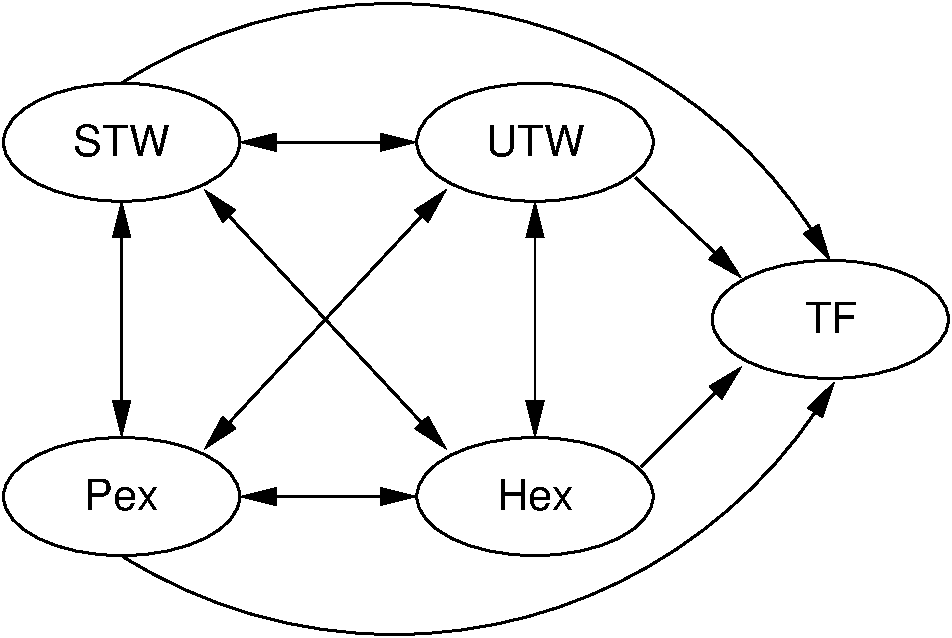
\includegraphics[height=3.5cm]{11.markov-models/figs/5state.pdf}}
\end{center}

\end{frame}


%### New page ############################################################

\begin{frame}

\frametitle{Data}

Estimate the Markov model transition probabilities using individual-level transition data

\bi
\item From a RCT with 2 treatments

\bi
\item SFC: Salmeterol (50$\mu$g) / fluticasone propionate (100$\mu$g) in combination
  \begin{itemize}
  \item new treatment, $t=2$
  \end{itemize}
\item FP: Fluticasone propionate alone (100$\mu$g) 
  \begin{itemize}
  \item existing treatment, $t=1$
  \end{itemize}
  \ei

\item 12 week trial

\item For each arm we count the number of transitions between states from week $j$ to $j+1$

\item From the Markov assumption, these can be considered independent
\ei

\end{frame}

%### New page ############################################################

\begin{frame}

\frametitle{Data}

\begin{center}
\begin{tabular}{l|rrrrr|r} \hline
\multicolumn{7}{c}{SFC} \\ \hline
&\multicolumn{5}{c|}{Number in state at week $j+1$}&Total in state \\
$r_{ss'}$&STW&UTW&Hex&Pex&TF&at week $j$ ($n_s$)\\ \hline
STW & 210 &  60 & 0 & 1 &  1 & 272 \\
UTW &  88 & 641 & 0 & 4 & 13 & 746 \\
Hex &   0 &   0 & 0 & 0 &  0 &   0 \\
Pex &   1 &   0 & 0 & 0 &  1 &   2 \\
TF  &   0 &   0 & 0 & 0 & 81 &  81 \\ \hline \hline
\multicolumn{7}{c}{FP} \\ \hline
STW &  66 &  32 & 0 & 0 &  2 & 100 \\
UTW &  42 & 752 & 0 & 5 & 20 & 819 \\
Hex &   0 &   0 & 0 & 0 &  0 &   0 \\
Pex &   0 &   4 & 0 & 1 &  0 &   5 \\
TF  &   0 &   0 & 0 & 0 &156 & 156 \\ \hline
\end{tabular}
\end{center}

These are summed over all weeks

\end{frame}

%### New page ############################################################

\begin{frame}

\frametitle{Estimating transition probabilities}


 Could estimate $(s,s')$ transition probability by dividing total 
\begin{itemize}
\item number of transitions observed from $s$ to $s'$, by 
\item number of weeks observed in state $s$ 
\end{itemize}

 But can't estimate transition rates out of Hex since nobody went
  into~Hex! \\
 Also very few went into Pex
  \begin{itemize}
  \item estimates / SEs for rates \alert{out of} Pex will be unstable.
  \end{itemize}

 Economic model needs to
  \begin{itemize}
  \item   include possibility of Hex / Pex --
  expensive states! 
\item account for \alert{uncertainty} in the transition
  rates.
  \end{itemize}



  $\rightarrow$ use Bayesian inference
  \begin{itemize}
  \item   -- combine \alert{priors} on
Hex/Pex/other states with data
\item  $\rightarrow$ \alert{posterior}
distribution of transition probabilities.
  \end{itemize}

\end{frame}

%### New page ############################################################

\begin{frame}

\frametitle{Binomial distribution for an event}

Suppose there are two states in the model (\emph{successfully treated
  week} / \emph{treatment failure}).

Out of $n$ people currently under treatment, the following week $r$
people have had treatment failure.

\begin{center}
\input{11.markov-models/figs/2state.pstex_t}
\end{center}

\begin{center}
\begin{tabular}{l||rr}
\hline
Total in STW at $j$ & \multicolumn{2}{c}{Number in state at $j+1$}\\
at week $j$ & STW & TF  \\ \hline
$n$ & $n-r$ & $r$ \\ \hline
\end{tabular}
\end{center}

Beta distribution is a convenient prior for $\lambda$ (conjugacy)

\end{frame}

%### New page ############################################################

%%%%%%\begin{frame}
%%%%%%
%%%%%%\frametitle{Bayesian estimation of binomial model}
%%%%%%
%%%%%%As in drug example, Lectures 1/2. \\ \alert{Likelihood} 
%%%%%%\[
%%%%%%\begin{array}{lllll}
%%%%%%r &\sim &\mbox{Binomial} (\lambda,n)&& \\
%%%%%%\displaystyle p(r\mid\lambda) &=& \frac{n!}{r!(n-r!)}\lambda^r(1-\lambda)^{n-r} &\propto& \lambda^r(1-\lambda)^{n-r}
%%%%%%\end{array}
%%%%%%\]
%%%%%%\alert{Prior}
%%%%%%\[
%%%%%%\begin{array}{lllll}
%%%%%%\lambda &\sim &\mbox{Beta} (a,b)&&  \\
%%%%%%\displaystyle p(\lambda) &=& \frac{\Gamma(a+b)}{\Gamma(a)\Gamma(b)}\lambda^{a-1}(1-\lambda)^{b-1} &\propto& \pi^{a-1}(1-\pi)^{b-1} 
%%%%%%\end{array}
%%%%%%\]
%%%%%%(e.g. prior ignorance: Beta(1,1): uniform (flat) prior on 0--1)
%%%%%%
%%%%%%\alert{Posterior}
%%%%%%\begin{eqnarray}
%%%%%%p(\lambda\mid r) &\propto& \lambda^{a+r-1}(1-\lambda)^{b+n-r-1} \nonumber \\
%%%%%%\lambda\mid r &\sim &\mbox{Beta} (a+r,b+n-r) \nonumber 
%%%%%%\end{eqnarray}
%%%%%%
%%%%%%
%%%%%%\end{frame}
%%%%%%


%### New page ############################################################

\begin{frame}

\frametitle{Multinomial model for several events}

\begin{center}
\input{11.markov-models/figs/5state-1row.pstex_t}
\end{center}

%$\sum \pi_j=1$ 

\begin{center}
\begin{tabular}{ccccc|c} \\ \hline
\multicolumn{5}{c|}{Number in state at $j+1$}&Total in STW at $j$ \\
STW&UTW&Hex&Pex&TF&at week $j$ \\ \hline
$r_1$ & $r_2$ & $r_3$ & $r_4$ &  $r_5$ & $n$ \\ \hline
\end{tabular}
\end{center}


\end{frame}

%### New page ############################################################

\begin{frame}

\frametitle{Bayesian estimation of multinomial model}
%\vspace{-1.5cm}

\textbf{Likelihood}
\myblue
\[
\begin{array}{lllll}
r_1, \ldots, r_5  &\sim &\multicolumn{3}{l}{\mbox{Multinomial} (\lambda_1, \ldots, \lambda_5,n)} \\
p(\bm r\mid\bm\lambda) &=& \frac{n!}{r_1! \cdots r_5!}\lambda_1^{r_1} \ldots \lambda_5^{r_5} &\propto& \lambda_1^{r_1} \ldots \lambda_5^{r_5} \\
\sum \lambda_s &=& 1
\end{array}
\]

\black  
\textbf{Prior distribution for five transition probabilities}
\myblue
\[
\begin{array}{lllll}
(\lambda_1,\ldots,\lambda_5) &\sim &\mbox{Dirichlet} (a_1,\ldots,a_5)&&  \\
p(\lambda_1,\ldots,\lambda_5) &=& \frac{\Gamma(a_1+\cdots+a_5)}{\Gamma(a_1)\cdots\Gamma(a_5)}\lambda_1^{(a_1-1)}\cdots\lambda_5^{(a_5-1)} &\propto& \lambda_1^{(a_1-1)}\cdots\lambda_5^{(a_5-1)} 
\end{array}
\] 

\black  
\textbf{Posterior distribution}
\myblue
\begin{eqnarray}
p(\bm\lambda\mid \bm r) &\propto& \lambda_1^{(a_1+r_1-1)}\cdots\lambda_5^{(a_5+r_5-1)} \nonumber \\
\bm\lambda &\sim & \mbox{Dirichlet} (a_1+r_1,\ldots, a_5+r_5)\nonumber 
\end{eqnarray}

\end{frame}

%### New page ############################################################
%%% NEED TO CHECK NOTATION FROM HERE!!!!

\begin{frame}

\frametitle{Dirichlet prior distribution}

\begin{itemize}
\item General prior for a set of numbers that add up to 1. 
\item[] $(p_1, \ldots, p_S) \sim \mbox{Dirichlet}(a_1, \ldots, a_S)$
\begin{itemize}
\item $a_s$ proportional to \alert{expected} probability $p_s$ of outcome $s$
\item scale of the $a_s$ indicates prior \alert{precision} of $(p_1, \ldots, p_S)$
\end{itemize}

\vspace{10pt}
\item \textbf{NB}: $\mbox{Dirichlet} (1,\ldots, 1)$ is a flat prior.
\item Given a sample size $\sum a_s$, $a_s$ is your prior expectation for the number
of patients you would expect in each state $s$
\end{itemize}

\end{frame}

%### New page ############################################################
%%%%%%
%%%%%%\begin{frame}
%%%%%%\frametitle{Coding this in \bugs}
%%%%%%\begin{itemize}
%%%%%%\item Use \bugs to sample from the posterior distribution of the transition probabilities. 
%%%%%%\item Data: counts of patients going from each state $r$ to each state $s$: a \alert{matrix}.
%%%%%%\end{itemize}
%%%%%%
%%%%%%The \texttt{structure} command in \openbugs and \winbugs is a structure for storing data
%%%%%%\texttt{structure(.Data=c(1,2,3,4,5,6),.Dim=c(2,3))}
%%%%%%
%%%%%%The rightmost index is filled first (read across columns, then rows)
%%%%%%so this is a matrix with 2 rows and 3 columns
%%%%%%
%%%%%%\[
%%%%%%\left(
%%%%%%\begin{array}{ccc}
%%%%%%[1,1] & [1,2] & [1,3] \\{}
%%%%%%[2,1] & [2,2] & [3,3] 
%%%%%%\end{array}
%%%%%%\right)
%%%%%%=
%%%%%%\left(
%%%%%%\begin{array}{ccc}
%%%%%%1 & 2 & 3\\
%%%%%%4 & 5 & 6 
%%%%%%\end{array}
%%%%%%\right)
%%%%%%\]
%%%%%%\end{frame}

%### New page ############################################################

%%%%\begin{frame}[fragile]
%%%%
%%%%\frametitle{Multinomial / Dirichlet model in \bugs}
%%%%
%%%%Assuming we don't know the formula for the Dirichlet posterior, we
%%%%could let BUGS sample from it given the prior and the data.  In this
%%%%example:
%%%%
%%%%{\footnotesize \olive
%%%%\begin{verbatim}
%%%%model {
%%%%## Multinomial distribution for r, 
%%%%## i=4 non-absorbing states
%%%%for(s in 1:(S-1)){
%%%%    r.sfc[s,1:S] ~ dmulti(lambda.sfc[s,1:S], n.sfc[s]) 
%%%%    r.fp[s,1:S] ~ dmulti(lambda.fp[s,1:S], n.fp[s])    
%%%%}
%%%%## Dirichlet prior distributions for the 
%%%%## transition probabilities lambda
%%%%for(s in 1:(S-1)){
%%%%    lambda.sfc[s,1:S] ~ ddirch(prior.sfc[s,1:S])
%%%%    lambda.fp[s,1:S] ~ ddirch(prior.fp[s,1:S])
%%%%}
%%%%## Fixed transition probabilities for the absorbing state - 
%%%%## prob 1 of staying there - prob 0 of moving
%%%%for(s in 1:S){
%%%%    lambda.sfc[S,s] <- p.fixed[s]
%%%%    lambda.fp[S,s] <- p.fixed[s]
%%%%}
%%%%} ## end of model
%%%%\end{verbatim}
%%%%}
%%%%\end{frame}

\begin{frame}[fragile]

\frametitle{Multinomial / Dirichlet model in \bugs \hspace{0pt plus 1filll}\small \textbf{(cfr BMHE, \S5.4.1)}}

{\footnotesize \olive
\begin{semiverbatim}
model \{
\blue# Multinomial distribution for r, s=1,...,4: non-absorbing states\olive
   for(s in 1:(S-1))\{
      r.sfc[s,1:S] \mytilde dmulti(lambda.sfc[s,1:S], n.sfc[s]) 
      r.fp[s,1:S] \mytilde dmulti(lambda.fp[s,1:S], n.fp[s])    
   \}

\blue# Dirichlet prior distributions for the transition probabilities lambda\olive
   for(s in 1:(S-1))\{
      lambda.sfc[s,1:S] \mytilde ddirch(prior.sfc[s,1:S])
      lambda.fp[s,1:S] \mytilde ddirch(prior.fp[s,1:S])
   \}

\blue# Fixed transition probabilities for the absorbing state - prob 1 of staying there/prob 0 of moving\olive 
   for(s in 1:S)\{
      lambda.sfc[S,s] <- p.fixed[s]
      lambda.fp[S,s] <- p.fixed[s]
   \}
\} 
\end{semiverbatim}
}
\end{frame}



\begin{frame}[fragile]

  \frametitle{Simulating from a Dirichlet in \R}

  However the Dirichlet posterior is known here. 

  We can simulate directly from a known Dirichlet distribution in \R by
  exploiting that a Dirichlet random vector is a function of Gamma
  random variables:
  \begin{itemize}
  \item Simulate $Z_s \sim \mbox{Gamma}(a_s, 1)$ for $s=1, \ldots, S$. Then
  \item $(Z_1, \ldots,  Z_S) / \sum_{i=1}^S Z_i \sim \mbox{Dirichlet} (a_1,\ldots,a_S)$
  \end{itemize}

  \pause
  
  For example, to simulate 1000 draws from a Dirichlet(1,1,1,1):

  {\footnotesize \olive
\begin{verbatim}
a <- c(1, 1, 1, 1)
dir_rand <- matrix(nrow=1000, ncol=4)
for (i in 1:4)
    dir_rand[,i] <- rgamma(1000, a[i], 1)
dir_rand <- dir_rand / rowSums(dir_rand)
\end{verbatim}
  }

  \pause
  
  Or functions to simulate directly from the Dirichlet are provided in several \R add-on packages available from CRAN, e.g.

  {\footnotesize \olive
\begin{verbatim}
install.packages("VGAM") # if not already installed
library(VGAM)
dir_rand <- rdiric(1000, a)
\end{verbatim}
}
  
\end{frame}


%%%%%%### New page ############################################################
%%%%%
%%%%%\begin{frame}[fragile]
%%%%%
%%%%%\frametitle{Markov model in \openbugs: data format}
%%%%%%\vspace{-5cm}
%%%%%\begin{verbatim}
%%%%%
%%%%%list(
%%%%%
%%%%%r.sfc=structure(.Data=c(210,60,0,1,1, 88,641,0,4,13, 
%%%%%                        0,0,0,0,0, 1,0,0,0,1),.Dim=c(4,5)),
%%%%%n.sfc=c(272,746,0,2),
%%%%%r.fp=structure(.Data=c(66,32,0,0,2, 42,752,0,5,20, 
%%%%%                       0,0,0,0,0, 0,4,0,1,0),.Dim=c(4,5)),
%%%%%n.fp=c(100,819,0,5),
%%%%%prior.sfc=structure(.Data=c(1,1,1,1,1, 1,1,1,1,1, 
%%%%%                            1,1,1,1,1, 1,1,1,1,1),.Dim=c(4,5)),
%%%%%prior.fp=structure(.Data=c(1,1,1,1,1, 1,1,1,1,1, 
%%%%%                           1,1,1,1,1, 1,1,1,1,1),.Dim=c(4,5)),
%%%%%p.fixed=c(0,0,0,0,1)
%%%%%
%%%%%)
%%%%%
%%%%%\end{verbatim}
%%%%%
%%%%%
%%%%%\end{frame}

%### New page ############################################################

%%%%%\begin{frame}
%%%%%
%%%%%\frametitle{Estimated transition probabilities}
%%%%%
%%%%%{\small
%%%%%\begin{center}
%%%%%\begin{tabular}{ll|rrrrr|r} \\ \hline
%%%%%&&\multicolumn{5}{c|}{To}&\\
%%%%%&$\pi_{ij}$&STW&UTW&Hex&Pex&TF&Total\\ \hline
%%%%%\multicolumn{8}{c}{SFC} \\ \hline
%%%%%    &STW & 0.762 & 0.220 & 0.004 & 0.007 & 0.007 & 1 \\
%%%%%    &UTW & 0.118 & 0.855 & 0.001 & 0.007 & 0.019 & 1 \\
%%%%%From&Hex & 0.200 & 0.200 & 0.200 & 0.200 & 0.200 & 1 \\
%%%%%    &Pex & 0.289 & 0.143 & 0.142 & 0.142 & 0.284 & 1 \\
%%%%%    &TF  &   0 &   0 & 0 & 0 & 1 &  1 \\ \hline \hline
%%%%%\multicolumn{8}{c}{FP} \\ \hline
%%%%%    &STW & 0.638 & 0.315 & 0.009 & 0.010 & 0.029 & 1 \\
%%%%%    &UTW & 0.052 & 0.914 & 0.001 & 0.007 & 0.026 & 1 \\
%%%%%From&Hex & 0.202 & 0.200 & 0.197 & 0.200 & 0.201 &   1 \\
%%%%%    &Pex & 0.100 & 0.501 & 0.100 & 0.200 & 0.099 &   1 \\
%%%%%    &TF  &  0 &   0 & 0 & 0 & 1 &  1 \\ \hline
%%%%%\end{tabular}
%%%%%\end{center}
%%%%%}
%%%%%\vfill \small
%%%%%\textbf{NB}: Means of the posterior distributions are shown here
%%%%%
%%%%%\end{frame}
%### New page ############################################################

\begin{frame}

\frametitle{Estimated transition probabilities versus observed data}
% \vspace{-2cm}

After obtaining the posterior Dirichet distributions
{\footnotesize

\begin{tabular}{l|rrrrr||rrrrr} \\ \hline
&\multicolumn{5}{c||}{\alert{Raw transition counts}} & \multicolumn{5}{c}{\alert{Bayesian posterior mean}} \\ \hline
    \textbf{To:}&STW&UTW&Hex&Pex&TF  &STW&UTW&Hex&Pex&TF\\ \hline
\textbf{From:}&\multicolumn{10}{c}{SFC} \\ \hline
 STW & 210 &  60 & 0 & 1 &  1 & 0.76 & 0.22 & 0.004 & 0.01 & 0.01  \\  
 UTW &  88 & 641 & 0 & 4 & 13 & 0.12 & 0.85 & 0.001 & 0.01 & 0.02  \\  
 Hex &   0 &   0 & 0 & 0 &  0 & 0.20 & 0.20 & 0.20 & 0.20 & 0.20   \\  
 Pex &   1 &   0 & 0 & 0 &  1 & 0.29 & 0.14 & 0.14 & 0.14 & 0.28   \\  
 TF  &   0 &   0 & 0 & 0 & 81 &   0 &   0 & 0 & 0 & 1              \\ 
 \hline
 &\multicolumn{10}{c}{FP} \\ \hline
 STW &  66 &  32 & 0 & 0 &  2 & 0.64 & 0.31 & 0.01 & 0.01 & 0.03   \\  
 UTW &  42 & 752 & 0 & 5 & 20 & 0.05 & 0.91 & 0.001 & 0.00 & 0.03  \\  
 Hex &   0 &   0 & 0 & 0 &  0 & 0.20 & 0.20 & 0.20 & 0.20 & 0.20   \\  
 Pex &   0 &   4 & 0 & 1 &  0 & 0.10 & 0.50 & 0.10 & 0.20 & 0.10   \\  
 TF  &   0 &   0 & 0 & 0 &156 &  0 &   0 & 0 & 0 & 1               \\ 
 \hline 
\end{tabular}
}

\vfill \small
Information from the prior has been combined with the data

\end{frame}


%### New page ############################################################

%%%%\begin{frame}
%%%%\frametitle{Cost effectiveness modelling}
%%%%
%%%%\begin{center}
%%%%\begin{overpic}[height=6.5cm]{10.markov-models/figs/5state-animation-1.png}
%%%%\only<2->{\put(0,0){\includegraphics[height=6.5cm]{10.markov-models/figs/5state-animation-2.png}}}
%%%%\only<3->{\put(0,0){\includegraphics[height=6.5cm]{10.markov-models/figs/5state-animation-3.png}}}
%%%%\only<4->{\put(0,0){\includegraphics[height=6.5cm]{10.markov-models/figs/5state-animation-4.png}}}
%%%%\end{overpic}
%%%%\end{center}
%%%%
%%%%\end{frame}

%### New page ############################################################

\begin{frame}
\frametitle{Cost-effectiveness modelling}

Calculate \alert{expected costs} and \alert{expected benefits} of each
treatment over the long term:

\begin{itemize}

\item \alert{Cohort simulation:} Estimate proportion of population in each state at each successive time
  (from Markov \emph{transition probabilities})
  \begin{itemize}
  \item at the start, everyone in ``base'' state (e.g. just received treatment) 
  \item usually in the long run, everyone will be in the ``absorbing'' state (e.g.~death)
  \end{itemize}
\vspace{10pt}

\item Assign cost and benefit to each state in model 
\vspace{10pt}

\item Accumulate expected cost and benefit over times

\end{itemize}

\vfill \footnotesize \textbf{NB}: Check BMHE 5.4 + practical!
  
\end{frame}

\frame{
\frametitle{Discounting}
\begin{itemize}

\item Costs and outcomes can occur at different times with respect to when the intervention is implemented

  \begin{itemize}

  \item Society tends to value benefits that arrive closer to the present time more than those that are achievable later in the future

  \end{itemize}

\item \alert{Discounting} accounts for differential timing by reducing the value of costs \& effects in the future

  \begin{itemize}

\item Particularly relevant for economic evaluation spanning over a time horizon $>$ 1 year (e.g. Markov models)
\end{itemize}

\pause

\item If cost at some future time $j$ is $c_{tj}$, then \alert{discounted} cost is $c_{tj}/(1+d)^j$.

\item Discount rate $d$: NICE suggest 3.5\% for costs and outcomes

\item \textbf{Present Value} of intervention (treatment) $t$ over a time horizon $J$ is \color{myblue}
\begin{eqnarray*}
\text{PV}^c_t = \sum_{j=0}^{J}\frac{c_{tj}}{(1+d)^j} \qquad \text{PV}^e_t = \sum_{j=0}^{J}\frac{e_{tj}}{(1+d)^j}
\end{eqnarray*} \color{black}
(for \color{blue}costs $c$ \color{black}and \color{red}clinical benefits $e$\color{black}, respectively)
\end{itemize}
}

%### New page ############################################################

\begin{frame}

\frametitle{Simulating prevalences of states over time}

\begin{itemize}
\item $\pi_{js}$ is the \textbf{expected proportion} of patients in state $s$ at time $j$
\item $\lambda_{ss'}$ is the probability of going from state $s$ to state $s'$ in one time step
\item Thus \myblue 
$$\pi_{j+1,s}=\pi_{j1}\lambda_{1s}+\cdots+\pi_{jS}\lambda_{Ss}$$
\black 
which we can write in matrix form as \myblue
\[
\begin{array}{rcl}
(\pi_{j+1,1},\ldots,\pi_{j+1,S})&=&(\pi_{j,1},\ldots,\pi_{j,S})
\left(
\begin{array}{ccc}
\lambda_{11} & \ldots & \lambda_{1S} \\
\vdots & \ddots & \vdots \\
\lambda_{S1} & \ldots & \lambda_{SS} 
\end{array}
\right) \nonumber \\
\bm{\pi}_{j+1}&=&\bm{\pi}_j \bm\Lambda
\end{array}
\]
\black 
\item \textbf{NB}: $\bm\Lambda$ may depend on time $j$

\pause

\item Instead of calculating \textbf{expected} proportions $\pi_{js}$, could
  simulate the \textbf{absolute number} $m_{js}$ of patients in a
  cohort of size $M$, in state $s$, at time $j$.
  \begin{itemize}
  \item may help to illustrate what model is doing, though decision is generally based on \alert{expected} cost (average cost for an infinite population)
  \end{itemize}
  
\end{itemize}





\end{frame}

% CJ 2019: remove BUGS code, as we don't recommend people use BUGS to do this 
% %### New page ############################################################

% \begin{frame}[fragile]

% \frametitle{Coding this in \bugs}

% {\footnotesize \olive
% \begin{verbatim}
% ## Starting state
% for(s in 1:S){
%     m.sfc[1,s] <- m.start[s]
%     m.fp[1,s]  <- m.start[s]
% }

% ## Markov model
% for(j in 2:J){
%     for(s in 1:S){  # state proportions
%         m.sfc[j,s] <- inprod(m.sfc[j-1,1:S],lambda.sfc[1:S,s]) 
%         m.fp[j,s]  <- inprod(m.fp[j-1,1:S],lambda.fp[1:S,s])
%     }
% }
% ## inprod(v1[1:5],v2[1:5]) = sum_{i=1 to 5} v1_i v2_i
% \end{verbatim}

% \vfill \black 
% \textbf{NB}: Probably best to leave this computation to \texttt{R}, once the simulations for \texttt{lambda.sfc} and \texttt{lambda.fp} are available!

% }
% \end{frame}

\begin{frame}[fragile]
\frametitle{Coding this in \texttt{R} \small{(see BMHE 5.4)}}

Markov cost-effectiveness models can be implemented straightforwardly in \R. 

{\footnotesize \olive
\begin{verbatim}
  pi_sfc <- pi_fp <- array(dim = c(n.sims, # number of PSA samples 
                              S,    # number of states 
                              J+1)) # number of times 
  for (i in 1:n_sims){                # Assumes only 1 patient
      pi_sfc[i,,1] <- c(1,0,0,0,0)    #  initially in the state 
      pi_fp[i,,1] <- c(1,0,0,0,0)     #  'In health'
  }

  for (i in 1:n.sims) {
      for (j in 2:(J+1)){
          for (s in 1:S){
              pi_sfc[i,s,j] <- sum(pi_sfc[i,,j-1]*lambda_sfc[i,,s])
              pi_fp[i,s,j] <- sum(pi_fp[i,,j-1]*lambda_fp[i,,s])
          }
      }
  }
\end{verbatim}
  
%% \vfill \black \textbf{NB}: \texttt{BUGS} increases variables by one dimension (scalars become vectors, vectors become matrices, matrices become arrays...)

}

Many different ways to write code like this: see the questions sheet / solutions for another way. \\

See also \texttt{heemod}, an \R package designed for health economic modelling \url{https://CRAN.R-project.org/package=heemod}

\end{frame}

%### New page ############################################################

\begin{frame}

\frametitle{Costs and utilities}
\begin{itemize}
\item Assign a cost to each state for each treatment
\begin{center}
\begin{tabular}{l|rrrrr} \\ \hline
&\multicolumn{5}{c}{Cost per week (\pounds)} \\
Treatment&STW&UTW&Hex&Pex&TF\\ \hline
SFC & 7.96 & 7.96 & 1821.17 & 100.79 & TF cost (j)\\
FP  & 2.38 & 2.38 & 1815.58 &  95.21 & TF cost (j)\\ \hline
\end{tabular}
\end{center}

\vspace{7pt}
\item In this example, assume the expected cost for week $j$ in SFC group is
$$\myblue \pi_{j1}\times\mathrm{cost}_{(SFC,1)}+\cdots + \pi_{j4}\times\mathrm{cost}_{(SFC,4)}+ \pi_{j5}\times\mbox{TF\:cost}(j) \vspace{-6pt}  \black$$
\begin{itemize}
\item $\displaystyle \myblue \mbox{TF\:cost}(j) = \pi_{j1}\mathrm{cost}_{(FP,1)}+ \cdots + \pi_{j4} \mathrm{cost}_{(FP,4)}$ $=$ average cost over states, weighted by probability of occupying state, under old treatment
\end{itemize}
\vspace{7pt}
\item Utility measure is the number of weeks in the successfully controlled state
\end{itemize}
\end{frame}

%### New page ############################################################

\begin{frame}[fragile]

\frametitle{Expected costs and effects from a Markov model in \R}
%\vspace{-1.5cm}

Combining probabilities of state occupancy (\texttt{pi\_sfc}) with state-specific costs and utilities, for SFC treatment group (with similar code for FP group)

{\footnotesize \olive
\begin{verbatim}
state_costs_sfc <- c(STW=7.96, UTW=7.96, Hex=1821.17, Pex=100.79, TF=NA)
state_util_sfc <- c(1, 0, 0, 0, 0)
cost_sfc <- eff_sfc <- numeric(nsim)

## Loop over PSA samples
for (i in 1:nsim){
    cts <- ets <- numeric(J)

    ## Loop over times j
    for (j in 1:J){
        state_costs_sfc["TF"] <- state_costs_sfc[1:4] %*% pi_sfc[i,1:3,j]
        # costs for time j, averaged over states
        cts[j] <- sum(pi_sfc[i,,j] * state_costs_sfc) 
        # effects for time j, averaged over states
        ets[j] <- sum(pi_sfc[i,,j] * state_util_sfc)  
    }
    # expected costs and effects summed over all times, and averaged over states
    # for PSA sample i
    cost_sfc[i] <- sum(cts) 
    eff_sfc[i] <- sum(ets) 
}
\end{verbatim}
}



%%% REMOVE BUGS CODE (CJ 2019) 

% {\footnotesize \olive
% \begin{verbatim}
% ## Cost at time j from Markov model 
% for(j in 2:J){
%     weekly.cost.tf.fp[j] <- ## cost of TF at time j
%         inprod(m.fp[j,1:4],weekly.cost.fp[1:4])/sum(m.fp[j,]) 
%     cost.sfc[j] <- inprod(m.sfc[j,1:4],weekly.cost.sfc[1:4])
%         + m.sfc[t,5]*weekly.cost.tf.fp[j]  
%     cost.fp[j]  <- inprod(m.fp[j,1:4],weekly.cost.fp[1:4])
%         + m.fp[t,5]*weekly.cost.tf.fp[j]
% }
% ## Costs and utilities
% mu.c[1] <- sum(cost.fp[2:J])
% mu.c[2] <- sum(cost.sfc[2:J])
% delta.c <- mu.c[2] - mu.c[1]
% mu.e[1] <- sum(m.fp[2:J,1])
% mu.e[2] <- sum(m.sfc[2:J,1])
% delta.e <- mu.e[2] - mu.e[1]
% \end{verbatim}
% }

% \vfill 
% \black \textbf{NB}: Again, can do this directly in \texttt{R} (see BMHE 5.4 + practical)!

\end{frame}

%### New page ############################################################

\begin{frame}[fragile]

\frametitle{Summary: Bayesian health economic model}
% \vspace{-1.5cm}

At each iteration of ``probabilistic sensitivity analysis'', for each arm 

\bi
\item \noindent\textbf{Step 1}: 
\bi
\item draw a realization of the transition probabilities $\bm\Lambda$ from their posterior distribution 
\item define starting state and set time $j=1$
\ei

\vspace{5pt}\pause
\item \noindent\textbf{Step 2}: Markov model
\bi
\item Set time $j = j+1$
\item find prevalence of states $\pi_j$ at this time
\item combine $\pi_j$ with state-specific cost and utility to calculate expected cost and utility at this time
\item repeat step 2 up to time horizon $j = J(=13$ in this case) 
\ei

\vspace{5pt}\pause
\item \noindent\textbf{Step 3}: Cost-effectiveness
\bi
\item calculate expected \alert{costs} 
\item calculate expected \alert{effects} (here, proportion of time spent in STW)
  \ei
  summed over times
  \ei

  Gives a sample from the \textbf{posterior distribution} of expected costs and effects:
  vectors \verb+cost_sfc, eff_sfc, cost_fp, eff_fp+ in R code
\end{frame}


%### New page ############################################################

\begin{frame}

\frametitle{Results}
%\vspace{-1.5cm}

Sample from \alert{joint posterior distribution} of costs and effects
for each treatment gives, e.g. 
\begin{itemize}
\item \alert{incremental cost-effectiveness ratio} = mean cost difference / mean benefit difference
\item ``cost-effectiveness plane''
\item incremental net benefit (with CI)
\item cost-effectiveness acceptability curve
\end{itemize}

\begin{center}
\rotatebox{0}{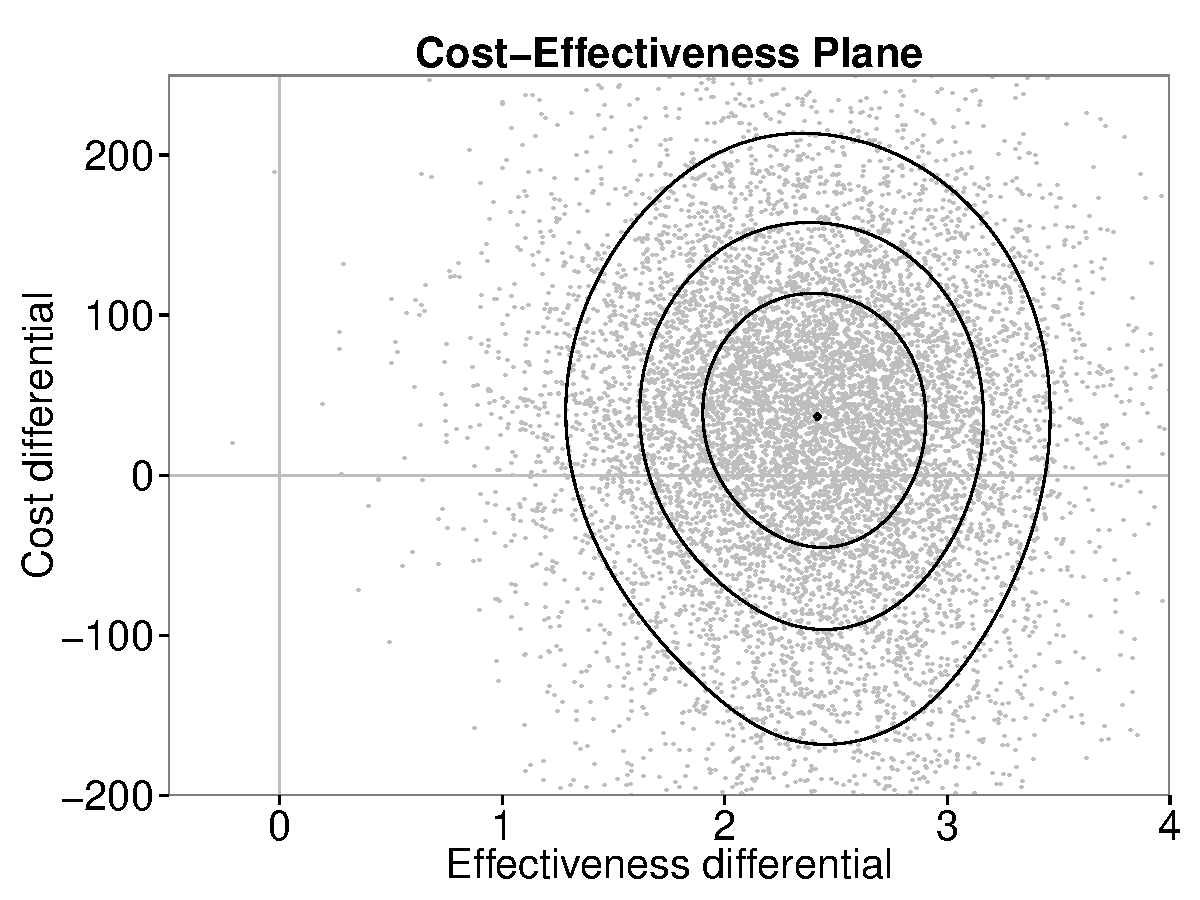
\includegraphics[height=4cm]{11.markov-models/figs/markov5-contour.pdf}}
\rotatebox{0}{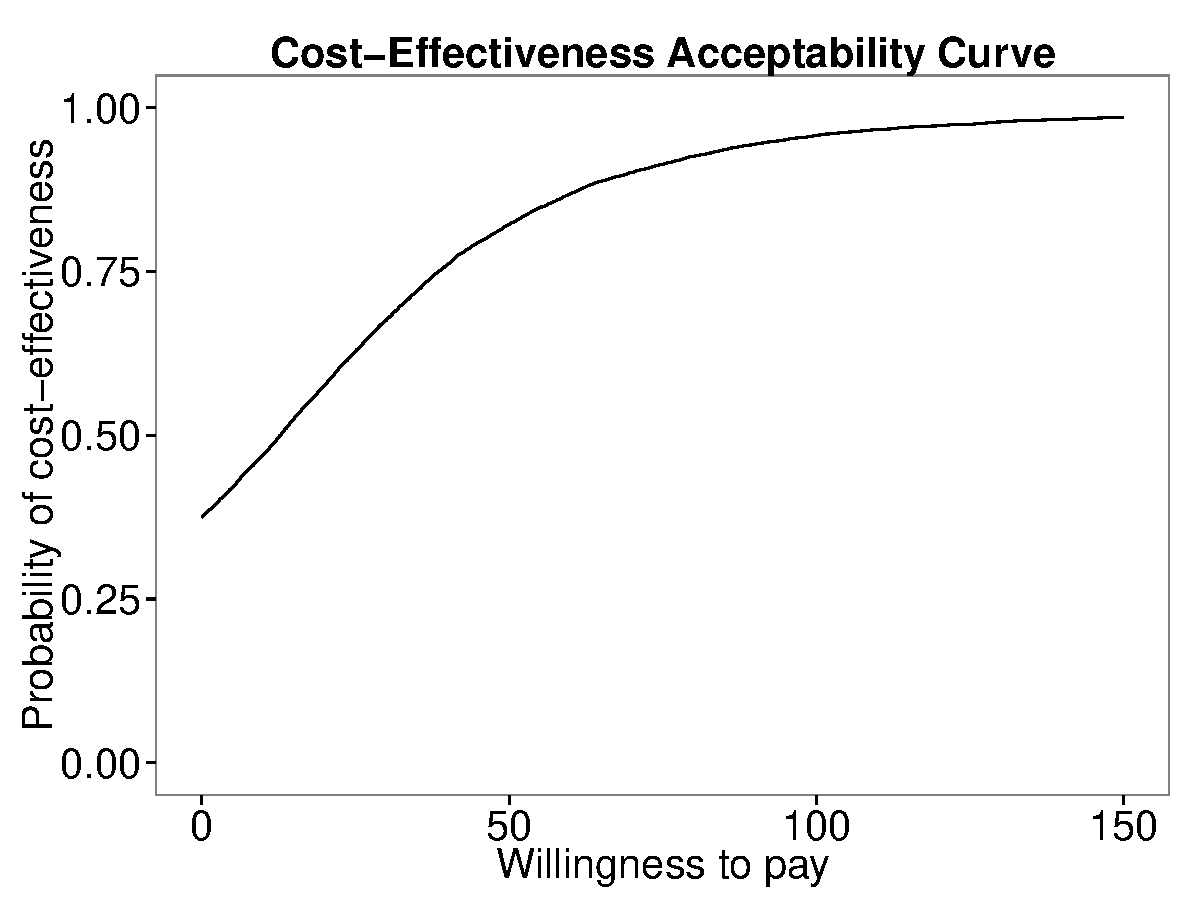
\includegraphics[height=4cm]{11.markov-models/figs//markov5-ceac.pdf}}
\end{center}

\end{frame}


\begin{frame}
  \frametitle{Bayesian decision modelling more generally}

  Example given here was simple
  \begin{itemize}
  \item Markov model with all transition probabilities estimated from
    individual-level transition count data.
  \end{itemize}

  Many more complicated examples, e.g. 

  \begin{itemize}

  \item Transition probabilities for baseline disease progression
    estimated from published data

  \item Treatment effects estimated from RCTs /
    (network-)meta-analysis $\rightarrow$ transition probabilities for
    treated groups

  \item Combinations of individual-level and published aggregate data$\ldots$

  \end{itemize}

  Examples in:
  \begin{itemize}
  \item   \bmhe,
  \item   \emph{Evidence Synthesis for Decision Making in Healthcare},
  \item   \url{http://nicedsu.org.uk/technical-support-documents/}
  \end{itemize}
 
\end{frame}


\begin{frame}

  \frametitle{Software strategy for Bayesian health economic modelling} 

  Typical health economic model:
  \begin{itemize}

  \item model is a \alert{deterministic
      function} $f(\theta)$ that transforms basic parameters $\theta$ to expected costs and effects for decision-making

  \item $\theta$ might include transition probabilities in a Markov
    model, or treatment effects (e.g. hazard ratios) that modify
    transition probabilities
  \end{itemize}

  \pause
  Typical software strategy:
  
 \begin{itemize}

 \item $\theta$ estimated from data using a Bayesian statistical model
   \begin{itemize}
   \item \texttt{BUGS} / \texttt{JAGS} / \texttt{Stan} ideal for this
   \item e.g. treatment effects estimated from network meta-analysis
   \end{itemize}
   $\rightarrow$ samples from the posterior distribution of $\theta$

   \pause 
  \item Export samples of $\theta$ to your preferred software for decision
    modelling
    \begin{itemize}
    \item e.g. \R, \texttt{Excel}
    \end{itemize}

  \item Calculate samples from the posterior of expected costs and effects
    $f(\theta)$
    \begin{itemize}
    \item a fully Bayesian decision model

  \item Asthma example can be done completely in \texttt{BUGS} (see practical material) but \texttt{BUGS} language cumbersome for programming harder models 

  \end{itemize}


  \end{itemize}

  \footnotesize
  \url{http://nicedsu.org.uk/technical-support-documents/evidence-synthesis-tsd-series/}:\\ TSD 6 ``Software choices''
  
\end{frame}


%%%%%%### New page ############################################################
%%%%% VERSION 2016
%%%%%
%%%%%\begin{frame}
%%%%%
%%%%%\frametitle{Summary}
%%%%%
%%%%%\bi
%%%%%\item Assess \alert{long-term} cost-effectiveness based only on
%%%%%  \alert{short-term} data.  
%%%%%
%%%%%\item State-transition (usually \emph{Markov}) models for clinical
%%%%%  histories.
%%%%%
%%%%%\item Commonly implemented in Excel, or specialized software (e.g. TreeAge).
%%%%%
%%%%%\item Bayesian framework lets you \alert{simultaneously} perform 
%%%%%  \begin{itemize}
%%%%%  \item parameter estimation (from short-term data, e.g. meta-analysis), and 
%%%%%  \item probabilistic sensitivity analysis (long-term costs and benefits)
%%%%%  \item - uncertainty about parameters fully included 
%%%%%  \end{itemize}
%%%%%
%%%%%\item Simple example: estimate transition probabilities using
%%%%%  \emph{multinomial} distribution in \bugs.
%%%%%
%%%%%\ei
%%%%%
%%%%%{\footnotesize \emph{Bayesian Methods in Health Economics} chapter 5.4}
%%%%%
%%%%%\end{frame}
%%%%%
%%%%%%### New page ############################################################
%%%%%
%%%%%\begin{frame}
%%%%%
%%%%%\frametitle{Asthma Example}
%%%%%
%%%%%(Briggs, Ades and Price. Medical Decision Making (2003);23:341-350)
%%%%%
%%%%%Five-state model for management of asthma:
%%%%%\bi
%%%%%\item STW: Successfully treated week
%%%%%\item UTW: Unsuccessfully treated week
%%%%%\item Hex: Hospital-managed exacerbation
%%%%%\item Pex: Primary care-managed exacerbation
%%%%%\item TF: Treatment failure - enters a ``usual care'' pattern (absorbing)
%%%%%\ei
%%%%%
%%%%%\begin{center}
%%%%%\rotatebox{0}{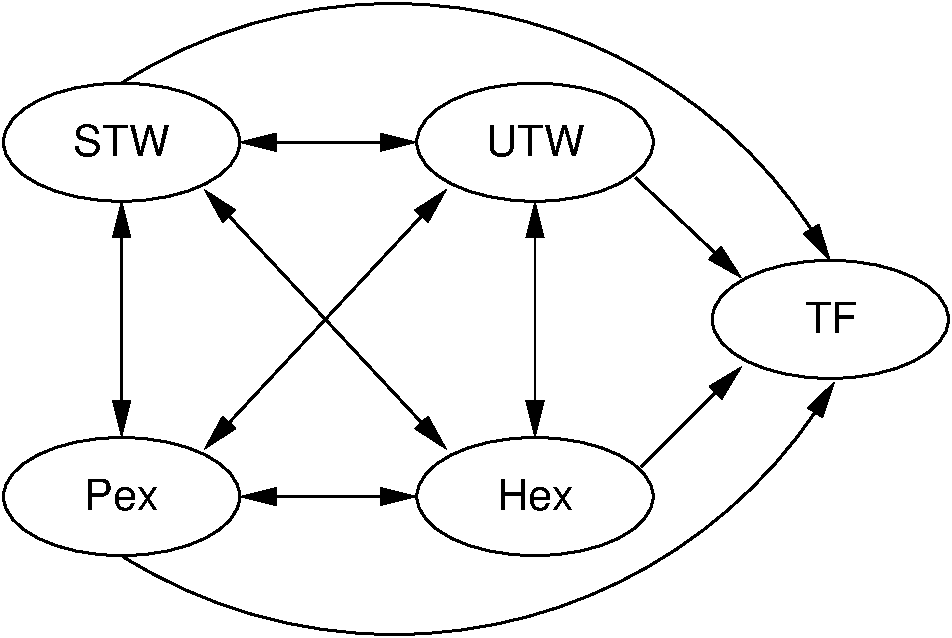
\includegraphics[height=3.5cm]{11.markov-models/figs/5state.pdf}}
%%%%%\end{center}
%%%%%
%%%%%\end{frame}
%%%%%
%%%%%%### New page ############################################################
%%%%%
%%%%%\begin{frame}
%%%%%
%%%%%\frametitle{Markov assumption (discrete time)}
%%%%%
%%%%%\alert{Markov} models are multi-state models in which next transition
%%%%%depends only on the current state
%%%%%
%%%%%\begin{eqnarray*}
%%%%%&&p(\mathrm{state} \: j \: \mathrm{at \: time} \: t+1\mid\mathrm{history \: of \: process})=  \\
%%%%%&&\qquad p(\mathrm{state} \: j \: \mathrm{at \: time} \: t+1\mid\mathrm{state} \: i \: \mathrm{at \: time} \:t)
%%%%%\end{eqnarray*}
%%%%%
%%%%%A Markov model is \alert{time-homogeneous} if this transition
%%%%%probability is the same for all times $t$.  
%%%%%\begin{itemize}
%%%%%\item Counterexample: risk of death depends on age.
%%%%%\end{itemize}
%%%%%
%%%%%\end{frame}
%%%%%
%%%%%%### New page ############################################################
%%%%%
%%%%%\begin{frame}
%%%%%
%%%%%\frametitle{Data}
%%%%%
%%%%%Data from a RCT with 2 treatments
%%%%%
%%%%%\bi
%%%%%\item SFC: Salmeterol (50$\mu$g) / fluticasone propionate (100$\mu$g) in combination (new treatment)
%%%%%\item FP: Fluticasone propionate alone (100$\mu$g) (existing treatment)
%%%%%\ei
%%%%%
%%%%%12 week trial
%%%%%
%%%%%For each arm we count the number of transitions between states from week $i$ to $i+1$
%%%%%
%%%%%From the Markov assumption, these can be considered independent.
%%%%%
%%%%%\end{frame}
%%%%%
%%%%%%### New page ############################################################
%%%%%
%%%%%\begin{frame}
%%%%%
%%%%%\frametitle{Data}
%%%%%
%%%%%\begin{center}
%%%%%\begin{tabular}{l|rrrrr|r} \hline
%%%%%\multicolumn{7}{c}{SFC} \\ \hline
%%%%%&\multicolumn{5}{c|}{Number in state at week $t+1$}&Total in state \\
%%%%%$r_{ij}$&STW&UTW&Hex&Pex&TF&at week $t$ ($n_i$)\\ \hline
%%%%%STW & 210 &  60 & 0 & 1 &  1 & 272 \\
%%%%%UTW &  88 & 641 & 0 & 4 & 13 & 746 \\
%%%%%Hex &   0 &   0 & 0 & 0 &  0 &   0 \\
%%%%%Pex &   1 &   0 & 0 & 0 &  1 &   2 \\
%%%%%TF  &   0 &   0 & 0 & 0 & 81 &  81 \\ \hline \hline
%%%%%\multicolumn{7}{c}{FP} \\ \hline
%%%%%STW &  66 &  32 & 0 & 0 &  2 & 100 \\
%%%%%UTW &  42 & 752 & 0 & 5 & 20 & 819 \\
%%%%%Hex &   0 &   0 & 0 & 0 &  0 &   0 \\
%%%%%Pex &   0 &   4 & 0 & 1 &  0 &   5 \\
%%%%%TF  &   0 &   0 & 0 & 0 &156 & 156 \\ \hline
%%%%%\end{tabular}
%%%%%\end{center}
%%%%%
%%%%%These are summed over all weeks
%%%%%
%%%%%\end{frame}
%%%%%
%%%%%%### New page ############################################################
%%%%%
%%%%%\begin{frame}
%%%%%
%%%%%\frametitle{Estimating transition probabilities}
%%%%%
%%%%%\begin{itemize}
%%%%%\item Could estimate $(r,s)$ transition probability by dividing total 
%%%%%\begin{itemize}
%%%%%\item number of transitions observed from $r$ to $s$, by 
%%%%%\item number of weeks observed in state $r$ 
%%%%%\end{itemize}
%%%%%
%%%%%\item But can't estimate transition rates out of Hex since nobody went
%%%%%  into Hex! 
%%%%%\item Also very few went into Pex -- estimates / SEs for rates out of
%%%%%  Pex will be unstable.
%%%%%\begin{itemize}
%%%%%\item Long-term economic model needs to include possibility of Hex /
%%%%%  Pex -- expensive states! 
%%%%%\item Needs to account for \alert{uncertainty} in the transition
%%%%%  rates.
%%%%%\end{itemize}
%%%%%
%%%%%\end{itemize}
%%%%%
%%%%%$\rightarrow$ use Bayesian inference -- combine \alert{priors} on
%%%%%Hex/Pex/other states with data $\rightarrow$ \alert{posterior}
%%%%%distribution of transition probabilities.
%%%%%
%%%%%\end{frame}
%%%%%
%%%%%%### New page ############################################################
%%%%%
%%%%%\begin{frame}
%%%%%
%%%%%\frametitle{Binomial distribution for an event}
%%%%%
%%%%%Suppose there are two states in the model (\emph{successfully treated
%%%%%  week} / \emph{treatment failure}).
%%%%%
%%%%%Out of $n$ people currently under treatment, the following week $r$
%%%%%people have had treatment failure.
%%%%%
%%%%%\begin{center}
%%%%%\input{11.markov-models/figs/2state.pstex_t}
%%%%%\end{center}
%%%%%
%%%%%\begin{center}
%%%%%\begin{tabular}{l||rr}
%%%%%\hline
%%%%%Total in STW at $t$ & \multicolumn{2}{c}{Number in state at $t+1$}\\
%%%%%at week $t$ & STW & TF  \\ \hline
%%%%%$n$ & $n-r$ & $r$ \\ \hline
%%%%%\end{tabular}
%%%%%\end{center}
%%%%%
%%%%%
%%%%%\end{frame}
%%%%%
%%%%%%### New page ############################################################
%%%%%
%%%%%\begin{frame}
%%%%%
%%%%%\frametitle{Bayesian estimation of binomial model}
%%%%%
%%%%%As in drug example, Lecture 3. \\ \alert{Likelihood} 
%%%%%\[
%%%%%\begin{array}{lllll}
%%%%%r &\sim &\mbox{Binomial} (\pi,n)&& \\
%%%%%\displaystyle p(r|\pi) &=& \frac{n!}{r!(n-r!)}\pi^r(1-\pi)^{n-r} &\propto& \pi^r(1-\pi)^{n-r}
%%%%%\end{array}
%%%%%\]
%%%%%\alert{Prior}
%%%%%\[
%%%%%\begin{array}{lllll}
%%%%%\pi &\sim &\mbox{Beta} (a,b)&&  \\
%%%%%\displaystyle p(\pi) &=& \frac{\Gamma(a+b)}{\Gamma(a)\Gamma(b)}\pi^{a-1}(1-\pi)^{b-1} &\propto& \pi^{a-1}(1-\pi)^{b-1} 
%%%%%\end{array}
%%%%%\]
%%%%%(e.g. prior ignorance: Beta(1,1): uniform (flat) prior on 0--1)
%%%%%
%%%%%\alert{Posterior}
%%%%%\begin{eqnarray}
%%%%%p(\pi|r) &\propto& \pi^{a+r-1}(1-\pi)^{b+n-r-1} \nonumber \\
%%%%%\pi|r &\sim &\mathrm{Beta} (a+r,b+n-r) \nonumber 
%%%%%\end{eqnarray}
%%%%%
%%%%%
%%%%%\end{frame}
%%%%%
%%%%%
%%%%%
%%%%%%### New page ############################################################
%%%%%
%%%%%\begin{frame}
%%%%%
%%%%%\frametitle{Multinomial model for several events}
%%%%%
%%%%%\begin{center}
%%%%%\input{11.markov-models/figs/5state-1row.pstex_t}
%%%%%\end{center}
%%%%%
%%%%%%$\sum \pi_j=1$ 
%%%%%
%%%%%\begin{center}
%%%%%\begin{tabular}{ccccc|c} \\ \hline
%%%%%\multicolumn{5}{c|}{Number in state at $t+1$}&Total in STW at $t$ \\
%%%%%STW&UTW&Hex&Pex&TF&at week $t$ \\ \hline
%%%%%$r_1$ & $r_2$ & $r_3$ & $r_4$ &  $r_5$ & $n$ \\ \hline
%%%%%\end{tabular}
%%%%%\end{center}
%%%%%
%%%%%
%%%%%\end{frame}
%%%%%
%%%%%%### New page ############################################################
%%%%%
%%%%%\begin{frame}
%%%%%
%%%%%\frametitle{Bayesian estimation of multinomial model}
%%%%%%\vspace{-1.5cm}
%%%%%
%%%%%Likelihood
%%%%%\[
%%%%%\begin{array}{lllll}
%%%%%r_1, \ldots, r_5  &\sim &\multicolumn{3}{l}{\mbox{Multinomial} (\pi_1, \ldots, \pi_5,n)} \\
%%%%%p(\bm r\mid\bm\pi) &=& \frac{n!}{r_1! \cdots r_5!}\pi_1^{r_1} \ldots \pi_5^{r_5} &\propto& \pi_1^{r_1} \ldots \pi_5^{r_5} \\
%%%%%\sum \pi_i &=& 1
%%%%%\end{array}
%%%%%\]
%%%%%Prior distribution for five transition probabilities
%%%%%\[
%%%%%\begin{array}{lllll}
%%%%%(\pi_1,\ldots,\pi_5) &\sim &\mbox{Dirichlet} (a_1,\ldots, a_5)&&  \\
%%%%%p(\pi_1,\ldots,\pi_5) &=& \frac{\Gamma(a_1+\cdots+a_5)}{\Gamma(a_1)\cdots\Gamma(a_5)}\pi_1^{(a_1-1)}\cdots\pi_5^{(a_5-1)} &\propto& \pi_1^{(a_1-1)}\cdots\pi_5^{(a_5-1)} 
%%%%%\end{array}
%%%%%\]
%%%%%Posterior distribution
%%%%%\begin{eqnarray}
%%%%%p(\bm\pi\mid \bm r) &\propto& \pi_1^{(a_1+r_1-1)}\cdots\pi_5^{(a_5+r_5-1)} \nonumber \\
%%%%%\bm\pi &\sim & \mbox{Dirichlet} (a_1+r_1,\ldots, a_5+r_5)\nonumber 
%%%%%\end{eqnarray}
%%%%%
%%%%%
%%%%%
%%%%%\end{frame}
%%%%%
%%%%%%### New page ############################################################
%%%%%
%%%%%\begin{frame}
%%%%%
%%%%%\frametitle{Dirichlet prior distribution}
%%%%%
%%%%%General prior for a set of numbers that add up to 1. 
%%%%%
%%%%%$(p_1, \ldots, p_m) \sim \mbox{Dirichlet}(a_1, \ldots, a_m)$
%%%%%\begin{itemize}
%%%%%\item $a_j$ proportional to \alert{expected} probability $p_j$ of outcome $j$
%%%%%\item scale of the $a_j$ indicates prior \alert{precision} of $(p_1, \ldots, p_m)$
%%%%%\end{itemize}
%%%%%
%%%%%$\mbox{Dirichlet} (1,\ldots, 1)$ is a flat prior.
%%%%%
%%%%%Given a sample size $\sum a_j$, $a_j$ is your prior expectation for the number
%%%%%of patients you would expect in each state $j$
%%%%%
%%%%%
%%%%%\end{frame}
%%%%%
%%%%%%### New page ############################################################
%%%%%
%%%%%\begin{frame}
%%%%%
%%%%%\frametitle{Coding this in \bugs}
%%%%%
%%%%%\begin{itemize}
%%%%%\item Use \bugs to sample from the posterior distribution of the transition probabilities. 
%%%%%
%%%%%\item Data: counts of patients going from each state $r$ to each state $s$: a \alert{matrix}.
%%%%%
%%%%%\end{itemize}
%%%%%
%%%%%
%%%%%The \texttt{structure} command in \openbugs and \winbugs is a structure for storing data
%%%%%
%%%%%\texttt{structure(.Data=c(1,2,3,4,5,6),.Dim=c(2,3))}
%%%%%
%%%%%The rightmost index is filled first (read across columns, then rows)
%%%%%so this is a matrix with 2 rows and 3 columns
%%%%%
%%%%%\[
%%%%%\left(
%%%%%\begin{array}{ccc}
%%%%%[1,1] & [1,2] & [1,3] \\{}
%%%%%[2,1] & [2,2] & [3,3] 
%%%%%\end{array}
%%%%%\right)
%%%%%=
%%%%%\left(
%%%%%\begin{array}{ccc}
%%%%%1 & 2 & 3\\
%%%%%4 & 5 & 6 
%%%%%\end{array}
%%%%%\right)
%%%%%\]
%%%%%
%%%%%\end{frame}
%%%%%
%%%%%%### New page ############################################################
%%%%%
%%%%%\begin{frame}[fragile]
%%%%%
%%%%%\frametitle{Markov model in \bugs}
%%%%%
%%%%%{\footnotesize 
%%%%%\begin{verbatim}
%%%%%model {
%%%%%## Multinomial distribution for r, 
%%%%%## i=4 non-absorbing states
%%%%%for(i in 1:4){
%%%%%    r.sfc[i,1:5] ~ dmulti(p.sfc[i,1:5], n.sfc[i]) 
%%%%%    r.fp[i,1:5] ~ dmulti(p.fp[i,1:5], n.fp[i])    
%%%%%}
%%%%%## Dirichlet prior distributions for the 
%%%%%## transition probabilities
%%%%%for(i in 1:4){
%%%%%    p.sfc[i,1:5] ~ ddirch(prior.sfc[i,1:5])
%%%%%    p.fp[i,1:5] ~ ddirch(prior.fp[i,1:5])
%%%%%}
%%%%%## Fixed transition probabilities for the absorbing state - 
%%%%%## prob 1 of staying there - prob 0 of moving
%%%%%for(j in 1:5){
%%%%%    p.sfc[5,j] <- p.fixed[j]
%%%%%    p.fp[5,j] <- p.fixed[j]
%%%%%}
%%%%%} ## end of model
%%%%%\end{verbatim}
%%%%%}
%%%%%\end{frame}
%%%%%
%%%%%%### New page ############################################################
%%%%%
%%%%%\begin{frame}[fragile]
%%%%%
%%%%%\frametitle{Markov model in \openbugs: data format}
%%%%%%\vspace{-5cm}
%%%%%\begin{verbatim}
%%%%%
%%%%%list(
%%%%%
%%%%%r.sfc=structure(.Data=c(210,60,0,1,1, 88,641,0,4,13, 
%%%%%                        0,0,0,0,0, 1,0,0,0,1),.Dim=c(4,5)),
%%%%%n.sfc=c(272,746,0,2),
%%%%%r.fp=structure(.Data=c(66,32,0,0,2, 42,752,0,5,20, 
%%%%%                       0,0,0,0,0, 0,4,0,1,0),.Dim=c(4,5)),
%%%%%n.fp=c(100,819,0,5),
%%%%%prior.sfc=structure(.Data=c(1,1,1,1,1, 1,1,1,1,1, 
%%%%%                            1,1,1,1,1, 1,1,1,1,1),.Dim=c(4,5)),
%%%%%prior.fp=structure(.Data=c(1,1,1,1,1, 1,1,1,1,1, 
%%%%%                           1,1,1,1,1, 1,1,1,1,1),.Dim=c(4,5)),
%%%%%p.fixed=c(0,0,0,0,1)
%%%%%
%%%%%)
%%%%%
%%%%%\end{verbatim}
%%%%%
%%%%%
%%%%%\end{frame}
%%%%%
%%%%%%### New page ############################################################
%%%%%
%%%%%\begin{frame}
%%%%%
%%%%%\frametitle{Estimated transition probabilities}
%%%%%
%%%%%{\small
%%%%%\begin{center}
%%%%%\begin{tabular}{ll|rrrrr|r} \\ \hline
%%%%%&&\multicolumn{5}{c|}{To}&\\
%%%%%&$\pi_{ij}$&STW&UTW&Hex&Pex&TF&Total\\ \hline
%%%%%\multicolumn{8}{c}{SFC} \\ \hline
%%%%%    &STW & 0.762 & 0.220 & 0.004 & 0.007 & 0.007 & 1 \\
%%%%%    &UTW & 0.118 & 0.855 & 0.001 & 0.007 & 0.019 & 1 \\
%%%%%From&Hex & 0.200 & 0.200 & 0.200 & 0.200 & 0.200 & 1 \\
%%%%%    &Pex & 0.289 & 0.143 & 0.142 & 0.142 & 0.284 & 1 \\
%%%%%    &TF  &   0 &   0 & 0 & 0 & 1 &  1 \\ \hline \hline
%%%%%\multicolumn{8}{c}{FP} \\ \hline
%%%%%    &STW & 0.638 & 0.315 & 0.009 & 0.010 & 0.029 & 1 \\
%%%%%    &UTW & 0.052 & 0.914 & 0.001 & 0.007 & 0.026 & 1 \\
%%%%%From&Hex & 0.202 & 0.200 & 0.197 & 0.200 & 0.201 &   1 \\
%%%%%    &Pex & 0.100 & 0.501 & 0.100 & 0.200 & 0.099 &   1 \\
%%%%%    &TF  &  0 &   0 & 0 & 0 & 1 &  1 \\ \hline
%%%%%\end{tabular}
%%%%%\end{center}
%%%%%}
%%%%%Means of the posterior distributions are shown here
%%%%%
%%%%%\end{frame}
%%%%%%### New page ############################################################
%%%%%
%%%%%\begin{frame}
%%%%%
%%%%%\frametitle{Estimated transition probabilities versus observed data}
%%%%%%\vspace{-2cm}
%%%%%{\footnotesize
%%%%%
%%%%%\begin{tabular}{l|rrrrr||rrrrr} \\ \hline
%%%%%
%%%%%&\multicolumn{5}{c||}{\alert{Raw transition counts}} & \multicolumn{5}{c}{\alert{Bayesian posterior mean}} \\ \hline
%%%%%    \textbf{To:}&STW&UTW&Hex&Pex&TF  &STW&UTW&Hex&Pex&TF\\ \hline
%%%%%\textbf{From:}&\multicolumn{10}{c}{SFC} \\ \hline
%%%%% STW & 210 &  60 & 0 & 1 &  1 & 0.76 & 0.22 & 0.004 & 0.01 & 0.01  \\  
%%%%% UTW &  88 & 641 & 0 & 4 & 13 & 0.12 & 0.85 & 0.001 & 0.01 & 0.02  \\  
%%%%% Hex &   0 &   0 & 0 & 0 &  0 & 0.20 & 0.20 & 0.20 & 0.20 & 0.20   \\  
%%%%% Pex &   1 &   0 & 0 & 0 &  1 & 0.29 & 0.14 & 0.14 & 0.14 & 0.28   \\  
%%%%% TF  &   0 &   0 & 0 & 0 & 81 &   0 &   0 & 0 & 0 & 1              \\ 
%%%%% \hline
%%%%% &\multicolumn{10}{c}{FP} \\ \hline
%%%%% STW &  66 &  32 & 0 & 0 &  2 & 0.64 & 0.31 & 0.01 & 0.01 & 0.03   \\  
%%%%% UTW &  42 & 752 & 0 & 5 & 20 & 0.05 & 0.91 & 0.001 & 0.00 & 0.03  \\  
%%%%% Hex &   0 &   0 & 0 & 0 &  0 & 0.20 & 0.20 & 0.20 & 0.20 & 0.20   \\  
%%%%% Pex &   0 &   4 & 0 & 1 &  0 & 0.10 & 0.50 & 0.10 & 0.20 & 0.10   \\  
%%%%% TF  &   0 &   0 & 0 & 0 &156 &  0 &   0 & 0 & 0 & 1               \\ 
%%%%% \hline 
%%%%%\end{tabular}
%%%%%}
%%%%%
%%%%%Information from the prior has been combined with the data. 
%%%%%
%%%%%\end{frame}
%%%%%
%%%%%
%%%%%%### New page ############################################################
%%%%%
%%%%%\begin{frame}
%%%%%\frametitle{Cost effectiveness modelling}
%%%%%
%%%%%\begin{center}
%%%%%\begin{overpic}[height=6.5cm]{11.markov-models/figs/5state-animation-1.png}
%%%%%\only<2->{\put(0,0){\includegraphics[height=6.5cm]{11.markov-models/figs/5state-animation-2.png}}}
%%%%%\only<3->{\put(0,0){\includegraphics[height=6.5cm]{11.markov-models/figs/5state-animation-3.png}}}
%%%%%\only<4->{\put(0,0){\includegraphics[height=6.5cm]{11.markov-models/figs/5state-animation-4.png}}}
%%%%%\end{overpic}
%%%%%\end{center}
%%%%%
%%%%%\end{frame}
%%%%%
%%%%%%### New page ############################################################
%%%%%
%%%%%\begin{frame}
%%%%%\frametitle{Cost effectiveness modelling}
%%%%%
%%%%%Calculate \alert{expected costs} and \alert{expected benefits} of each
%%%%%treatment over the long term:
%%%%%
%%%%%\begin{itemize}
%%%%%
%%%%%\item Assign cost and benefit to each state in model. 
%%%%%
%%%%%\item \alert{Cohort simulation:} Estimate proportion of population in each state at each successive time
%%%%%  (from Markov \emph{transition probabilities})
%%%%%  \begin{itemize}
%%%%%  \item at the start, everyone in ``base'' state (e.g. just received treatment) 
%%%%%  \item usually in the long run, everyone will be in the ``absorbing'' state (e.g. death)
%%%%%  \end{itemize}
%%%%%
%%%%%\item Accumulate expected cost and benefit over times. 
%%%%%
%%%%%\end{itemize}
%%%%%  
%%%%%\end{frame}
%%%%%
%%%%%\frame{
%%%%%\frametitle{Discounting}
%%%%%\begin{itemize}
%%%%%\item Costs and outcomes can occur at different times with respect to when the intervention is implemented
%%%%%\begin{itemize}
%%%%%\item Society tends to value benefits that arrive closer to the present time more than those that are achievable later in the future
%%%%%\end{itemize}
%%%%%\item \alert{Discounting} accounts for differential timing by reducing the value of costs \& effects in the future
%%%%%\begin{itemize}
%%%%%\item Particularly relevant for economic evaluation spanning over a time horizon $>$ 1 year (eg Markov models)
%%%%%\end{itemize}
%%%%%\item Define a discount rate $d$ (NICE suggest 3.5\% for costs and outcomes) and compute the \textbf{Present Value} of intervention (treatment) $t$ as \color{myblue}
%%%%%\begin{eqnarray*}
%%%%%\text{PV}^c_t = \sum_{j=0}^{J}\frac{c_{tj}}{(1+d)^j} \qquad \text{PV}^e_t = \sum_{j=0}^{J}\frac{e_{tj}}{(1+d)^j}
%%%%%\end{eqnarray*} \color{black}
%%%%%(for \color{blue}costs $c$ \color{black}and \color{red}clinical benefits $e$\color{black}, respectively)
%%%%%\end{itemize}
%%%%%}
%%%%%
%%%%%%### New page ############################################################
%%%%%
%%%%%\begin{frame}
%%%%%
%%%%%\frametitle{Simulating prevalences of states over time}
%%%%%
%%%%%$s_{jt}$ is the proportion of patients in state $j$ at time $t$
%%%%%
%%%%%$\pi_{ij}$ is the probability of going for state $i$ to state $j$ in one time step
%%%%%
%%%%%So $s_{t+1,j}=s_{t1}\pi_{1j}+\cdots+s_{t5}\pi_{5j}$
%%%%%
%%%%%Which we can write in matrix form as
%%%%%\[
%%%%%\begin{array}{rcl}
%%%%%(s_{t+1,1},\ldots,s_{t+1,5})&=&(s_{t,1},\ldots,s_{t,5})
%%%%%\left(
%%%%%\begin{array}{ccc}
%%%%%\pi_{11} & \ldots & \pi_{15} \\
%%%%%\vdots & \ddots & \vdots \\
%%%%%\pi_{51} & \ldots & \pi_{55} 
%%%%%\end{array}
%%%%%\right) \nonumber \\
%%%%%s_{t+1}^T&=&s_t^T \Pi
%%%%%\end{array}
%%%%%\]
%%%%%
%%%%%\end{frame}
%%%%%
%%%%%%### New page ############################################################
%%%%%
%%%%%\begin{frame}[fragile]
%%%%%
%%%%%\frametitle{Coding this in \bugs}
%%%%%
%%%%%{\footnotesize 
%%%%%\begin{verbatim}
%%%%%## Starting state
%%%%%for(j in 1:5){
%%%%%    s.sfc[1,j] <- s.start[j]
%%%%%    s.fp[1,j]  <- s.start[j]
%%%%%}
%%%%%
%%%%%## Markov model
%%%%%for(t in 2:13){
%%%%%    for(j in 1:5){  # state proportions
%%%%%        s.sfc[t,j] <- inprod(s.sfc[t-1,1:5],p.sfc[1:5,j]) 
%%%%%        s.fp[t,j]  <- inprod(s.fp[t-1,1:5],p.fp[1:5,j])
%%%%%    }
%%%%%}
%%%%%## inprod(v1[1:5],v2[1:5]) = sum_{i=1 to 5} v1_i v2_i
%%%%%## can also use inprod2 which is faster (and not documented)
%%%%%\end{verbatim}
%%%%%}
%%%%%
%%%%%\end{frame}
%%%%%
%%%%%%### New page ############################################################
%%%%%
%%%%%\begin{frame}
%%%%%
%%%%%\frametitle{Costs and utilities}
%%%%%
%%%%%Assign a cost to each state for each treatment
%%%%%
%%%%%\begin{center}
%%%%%\begin{tabular}{l|rrrrr} \\ \hline
%%%%%&\multicolumn{5}{c}{Cost per week (\pounds)} \\
%%%%%Treatment&STW&UTW&Hex&Pex&TF\\ \hline
%%%%%SFC & 7.96 & 7.96 & 1821.17 & 100.79 & TF cost (t)\\
%%%%%FP  & 2.38 & 2.38 & 1815.58 &  95.21 & TF cost (t)\\ \hline
%%%%%\end{tabular}
%%%%%\end{center}
%%%%%
%%%%%Total cost for week $t$ in SFC group is
%%%%%$s_{t1}\mathrm{cost}_{(SFC,1)}+\cdots + s_{t4} \mathrm{cost}_{(SFC,4)}+ s_{t5} \mathrm{TF\:cost}(t)$
%%%%%
%%%%%\vspace{0.25cm}
%%%%%
%%%%%where $\mathrm{TF\:cost}(t) = \frac{s_{t1}\mathrm{cost}_{(FP,1)}+ \cdots + s_{t4} \mathrm{cost}_{(FP,4)}}{s_{t1}+ \cdots +s_{t4}}$
%%%%%{\small (average cost over states, weighted by time spent in each state, under old treatment)}
%%%%%
%%%%%\vspace{0.25cm}
%%%%%
%%%%%Utility measure is the number of weeks in the successfully controlled state
%%%%%
%%%%%\end{frame}
%%%%%
%%%%%%### New page ############################################################
%%%%%
%%%%%\begin{frame}[fragile]
%%%%%
%%%%%\frametitle{Coding this in \bugs}
%%%%%%\vspace{-1.5cm}
%%%%%
%%%%%{\footnotesize 
%%%%%\begin{verbatim}
%%%%%## Cost at time t from Markov model 
%%%%%for(t in 2:13){
%%%%%    weekly.cost.tf.fp[t] <- ## cost of TF at time t
%%%%%        inprod(s.fp[t,1:4],weekly.cost.fp[1:4])/sum(s.fp[t,]) 
%%%%%    cost.sfc[t] <- inprod(s.sfc[t,1:4],weekly.cost.sfc[1:4])
%%%%%        + s.sfc[t,5]*weekly.cost.tf.fp[t]  
%%%%%    cost.fp[t]  <- inprod(s.fp[t,1:4],weekly.cost.fp[1:4])
%%%%%        + s.fp[t,5]*weekly.cost.tf.fp[t]
%%%%%}
%%%%%## Costs and utilities
%%%%%mu.c[1] <- sum(cost.fp[2:13])
%%%%%mu.c[2] <- sum(cost.sfc[2:13])
%%%%%delta.c <- mu.c[2] - mu.c[1]
%%%%%mu.e[1] <- sum(s.fp[2:13,1])
%%%%%mu.e[2] <- sum(s.sfc[2:13,1])
%%%%%delta.e <- mu.e[2] - mu.e[1]
%%%%%\end{verbatim}
%%%%%}
%%%%%
%%%%%\end{frame}
%%%%%
%%%%%%### New page ############################################################
%%%%%
%%%%%\begin{frame}
%%%%%
%%%%%\frametitle{At each iteration of the MCMC sampler}
%%%%%%\vspace{-1.5cm}
%%%%%
%%%%%\begin{description}
%%%%%\item[Step 1] Set up
%%%%%\bi
%%%%%\item draw a realization of the transition probabilities $\Pi$ from their posterior distribution 
%%%%%\item define starting state and set $t=1$
%%%%%\ei
%%%%%
%%%%%\item[Step 2] Markov model
%%%%%\bi
%%%%%\item $t=t+1$
%%%%%\item find state proportions $s_t$ in each arm
%%%%%\item find cost of these state proportions in each arm
%%%%%\item repeat step 2 until $t=13$
%%%%%\ei
%%%%%
%%%%%\item[Step 3] Cost-effectiveness
%%%%%\bi
%%%%%\item find total \alert{costs} in each arm
%%%%%\item find total \alert{benefit} (proportion of time spent in STW) in each arm
%%%%%\ei
%%%%%\end{description}
%%%%%
%%%%%\end{frame}
%%%%%
%%%%%
%%%%%%### New page ############################################################
%%%%%
%%%%%\begin{frame}
%%%%%
%%%%%\frametitle{Results}
%%%%%%\vspace{-1.5cm}
%%%%%
%%%%%Sample from \alert{joint posterior distribution} of costs and effects
%%%%%for each treatment gives, e.g. 
%%%%%\begin{itemize}
%%%%%\item \alert{incremental cost-effectiveness ratio} = mean cost difference / mean benefit difference
%%%%%\item ``cost-effectiveness plane''
%%%%%\item incremental net benefit (with CI)
%%%%%\item cost-effectiveness acceptability curve
%%%%%\end{itemize}
%%%%%
%%%%%\begin{center}
%%%%%\rotatebox{0}{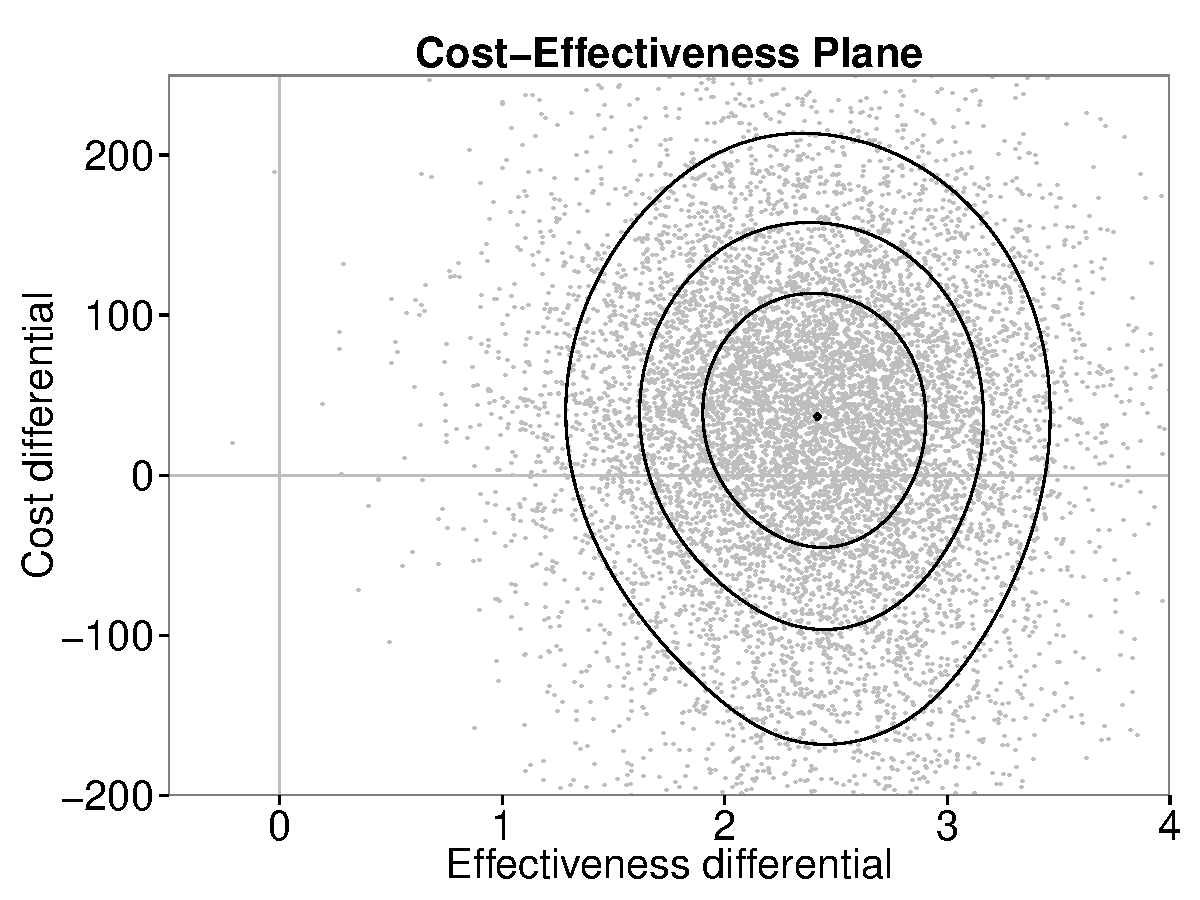
\includegraphics[height=4cm]{11.markov-models/figs/markov5-contour.pdf}}
%%%%%\rotatebox{0}{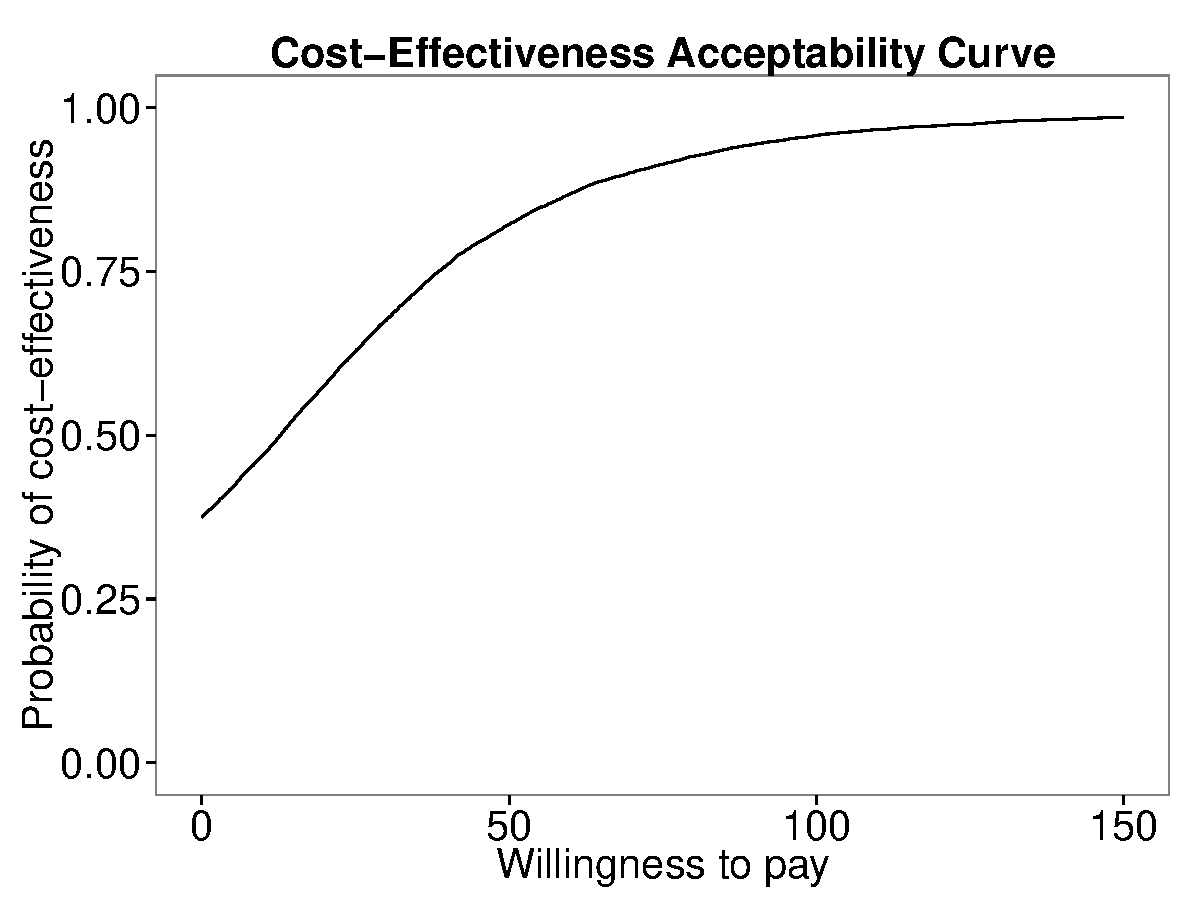
\includegraphics[height=4cm]{11.markov-models/figs//markov5-ceac.pdf}}
%%%%%\end{center}
%%%%%
%%%%%\end{frame}
%%%%%
%%%%%
%%%%%
%%%%%
%%%%%
%%%%%%### New page ############################################################
%%%%%
%%%%%\begin{frame}
%%%%%
%%%%%\frametitle{Using \bugs in general health economic models}
%%%%%
%%%%%Typical decision models developed in spreadsheets, evidence based on meta-analysis 
%%%%%
%%%%%\bi
%%%%%\item Could do Asthma model entirely in Excel because the posterior is
%%%%%  available in closed form
%%%%%
%%%%%\item \bugs needed for more complex meta-analysis / evidence
%%%%%  syntheses.
%%%%%
%%%%%\item $\ldots$ but not necessarily the easiest software for decision modelling 
%%%%%
%%%%%\item Combine the advantages of Bayesian inference with the
%%%%%  familiarity of a spreadsheet --- \alert{use \bugs output in
%%%%%    Excel$\ldots$}
%%%%%\ei
%%%%%
%%%%%\end{frame}
%%%%%
%%%%%\begin{frame}
%%%%%  \frametitle{Using \bugs output in a spreadsheet model}
%%%%%  \begin{itemize}
%%%%%  \item \texttt{Inference->Samples->coda} button in \openbugs generates
%%%%%    posterior sample for all monitored variables
%%%%%
%%%%%  \item Manipulate this awkward format into one column per variable 
%%%%%    \begin{itemize}
%%%%%    \item e.g. by using R  \texttt{coda} package
%%%%%    \item or, \emph{BUS --- BUGS Utility for Spreadsheets}. \url{http://faculty.salisbury.edu/~edhahn/bus.htm}
%%%%%    \end{itemize}
%%%%%
%%%%%\begin{center}
%%%%%\rotatebox{0}{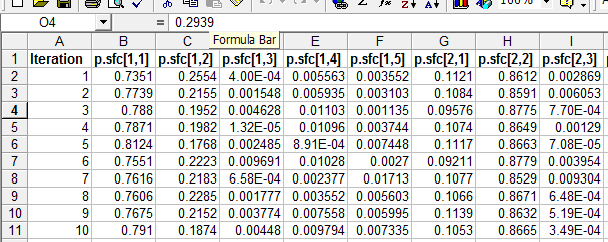
\includegraphics[height=3.5cm]{11.markov-models/figs/bugsout.png}}
%%%%%\end{center}
%%%%%
%%%%%\item
%%%%%  In one iteration of probabilistic sensitivity analysis --- take parameter values from the same MCMC iteration.     
%%%%%  \end{itemize}
%%%%%
%%%%%\end{frame}
%%%%%
%%%%%\begin{frame}
%%%%%
%%%%%\frametitle{Advantages of fully Bayesian economic models}
%%%%%
%%%%%Using posterior distributions from \bugs:
%%%%%\bi 
%%%%%
%%%%%\item Gives an \alert{exact} posterior representing parameter
%%%%%  uncertainties
%%%%%  \begin{itemize}
%%%%%  \item instead of Normal/beta/etc. approximations used in typical
%%%%%    probabilistic spreadsheet model
%%%%%  \end{itemize}
%%%%%
%%%%%\item Accounts for \alert{correlations} between parameters
%%%%%  \begin{itemize}
%%%%%  \item instead of common assumption that uncertainty distributions
%%%%%    are independent
%%%%%  \end{itemize}
%%%%%
%%%%%\ei
%%%%%
%%%%%See NICE Decision Support Unit technical document: \emph{Embedding evidence synthesis in probabilistic cost-effectiveness analysis: software choices} from \url{http://www.nicedsu.org.uk}
%%%%%  
%%%%%\end{frame}
%%%%%
%%%%%
%%%%%
%%%%%%### New page ############################################################
%%%%%
%%%%%\begin{frame}
%%%%%
%%%%%\frametitle{Further reading: continuous-time Markov models}
%%%%%
%%%%%\begin{itemize}
%%%%%\item \alert{Discrete-time} models -- health state can only change at the
%%%%%  start of the \emph{cycle} (e.g. week / month).  May be good
%%%%%  approximation
%%%%%
%%%%%\item \alert{Continuous-time} models -- can change state at any time --
%%%%%  more realistic, though mathematically harder. 
%%%%%
%%%%%  \begin{itemize}
%%%%%
%%%%%  \item Expressed in terms of \emph{transition intensities} (like the
%%%%%    \emph{hazard} in survival analysis), giving instantaneous
%%%%%    \emph{rate} of moving to each other state -- use to calculate
%%%%%    probability of occupying each state a given time in the future.
%%%%%
%%%%%  \item See Welton et al. \emph{Evidence Synthesis for Decision Making
%%%%%      in Healthcare} (Wiley, 2012), for methods and WinBUGS examples.
%%%%%
%%%%%  \item Also \texttt{msm} package for the R software (Jackson et al.,
%%%%%    2003) for fitting them to disease progression data.
%%%%%
%%%%%  \end{itemize}
%%%%%
%%%%%\end{itemize}
%%%%%
%%%%%\end{frame}
%%%%%
%%%%%
%%%%%%### New page ############################################################
%%%%%
%%%%%
%%%%%\begin{frame}
%%%%%  \frametitle{Practical: Markov Models} 
%%%%%
%%%%%  \textbf{Objectives}
%%%%%
%%%%%  \begin{itemize}
%%%%%
%%%%%  \item In the drug example in Lecture 3, we determined the exact
%%%%%    posterior distribution for the probability of an event after
%%%%%    observing data (Beta prior / Binomial likelihood), using:
%%%%%    \begin{itemize}
%%%%%    \item Monte Carlo in \bugs to simulate from the known posterior
%%%%%    \item MCMC in \bugs to simulate indirectly from it, given
%%%%%      data
%%%%%    \end{itemize}
%%%%%
%%%%%  \item Here we determine an exact posterior distribution for a
%%%%%    \alert{set} of probabilities for \alert{mutually exclusive}
%%%%%    events: the state in the next week, using
%%%%%    \begin{itemize}
%%%%%    \item Monte Carlo in \bugs to simulate from the known posterior
%%%%%    \item MCMC in \bugs to simulate indirectly from it, given
%%%%%      data
%%%%%    \end{itemize}
%%%%%
%%%%%  \item Forming a simplified Markov model by merging states
%%%%%    \begin{itemize}
%%%%%    \item performing cost-effectiveness analysis using this model. 
%%%%%    \end{itemize}
%%%%%
%%%%%
%%%%%  \end{itemize}
%%%%%
%%%%%  
%%%%%\end{frame}
%%%%%
%%%%%
%%%%%%%% Local Variables:
%%%%%%%% mode: latex
%%%%%%%% TeX-master: "../talks_cjtmp"
%%%%%%%% End:
 \nologo

\part{Uncertainty analysis}\label{psa} \frame{\partpage} \UCL
%%%%\setbeamerfont{itemize/enumerate body}{size*={9}{11}}
%%%%\setbeamerfont{itemize/enumerate subbody}{size*={8}{10}}
%%%%\setbeamerfont{itemize/enumerate subsubbody}{size*={7}{9}}

\frame{%
\frametitle{Handling uncertainty in economic evaluations}
\begin{itemize}
\item Population uncertainty: Sub-group analysis
\item Parameter uncertainty: Sensitivity analysis
\item Structural uncertainty: Sensitivity analysis
\item Collect more data
\item Sensitivity analysis (SA)
\item Deterministic sensitivity analysis
\begin{itemize}
	\item One-way SA
	\item Two-way SA
	\item Scenario analysis (best or worst case, what if..)
\end{itemize}
\item Probabilistic sensitivity analysis (PSA)
\begin{itemize}
	\item Monte Carlo simulation
\end{itemize}
\item Cost-effectiveness acceptability curves (CEAC)
\end{itemize}

}

\frame{%
\frametitle{How robust are health economic evaluations}
\begin{itemize}
\item Do limitations in either the quality or availability of evidence affect the recommended decision?
\item If the decision is not altered despite ‘reasonable’ variations in key assumptions/parameters, then the analysis can be considered to be ‘robust’
\item Two types of uncertainty:
\begin{itemize}
	\item Structural (is the model design correct?)
	\item Parameter (are the values correct?)
\end{itemize}
\item In economic evaluation, some form of sensitivity analysis is frequently carried out in order to allow for uncertainty
\item This uncertainty may be present in the evaluation for several reasons:
\begin{itemize}
	\item Data are unavailable and assumptions are necessary
	\item Available but inaccurate
\end{itemize}
\item In this type of analysis the	values recorded for important parameters are varied, usually one at a time, in order to determine whether the results are sensitive to the assumptions made
\end{itemize}
}

\frame{%
\frametitle{Uncertainty in economic evaluations}
\begin{itemize}
\item Structural: scenario analysis
\item Re-run the analysis with alternate assumptions and model structures
\item Parameter: sensitivity analysis (SA)
\item Re-run the analysis with different parameter values
\item Type of sensitivity analysis:
\begin{itemize}
	\item One-way SA
	\item Multi-way SA
	\item Extreme values SA
	\item Probabilistic SA
\end{itemize}
\end{itemize}
}

\frame{%
\frametitle{Types of sensitivity analysis}
\begin{itemize}
\item Simple sensitivity analysis entails varying one or more of the components of an evaluation to see how it affects the results
\item  Probabilistic sensitivity analysis assigns ranges and distribution to  variables and computer programs  are used to select values at  random from each range and to record the results
\item By using these different methods of sensitivity analysis it is possible to show whether the results of a particular study	over a range of  assumptions or hinge on the accuracy of particular assumptions
\end{itemize}
}

\frame{%
\frametitle{Uncertainty in economic evaluations}
\begin{itemize}
\item xxx
\end{itemize}

\vfill
\begin{block}{\footnotesize References}
\bmhe, chapter 1.\\
\bceabook
\end{block}

}

\frame{%
\frametitle{Uncertainty in economic evaluations}
\begin{itemize}
\item xxx
\end{itemize}

\vfill
\begin{block}{\footnotesize References}
\bmhe, chapter 1.\\
\bceabook
\end{block}

}

\frame{%
\frametitle{Uncertainty in economic evaluations}
\begin{itemize}
\item xxx
\end{itemize}

\vfill
\begin{block}{\footnotesize References}
\bmhe, chapter 1.\\
\bceabook
\end{block}

}

\frame{
\frametitle{A two input example}
\begin{center}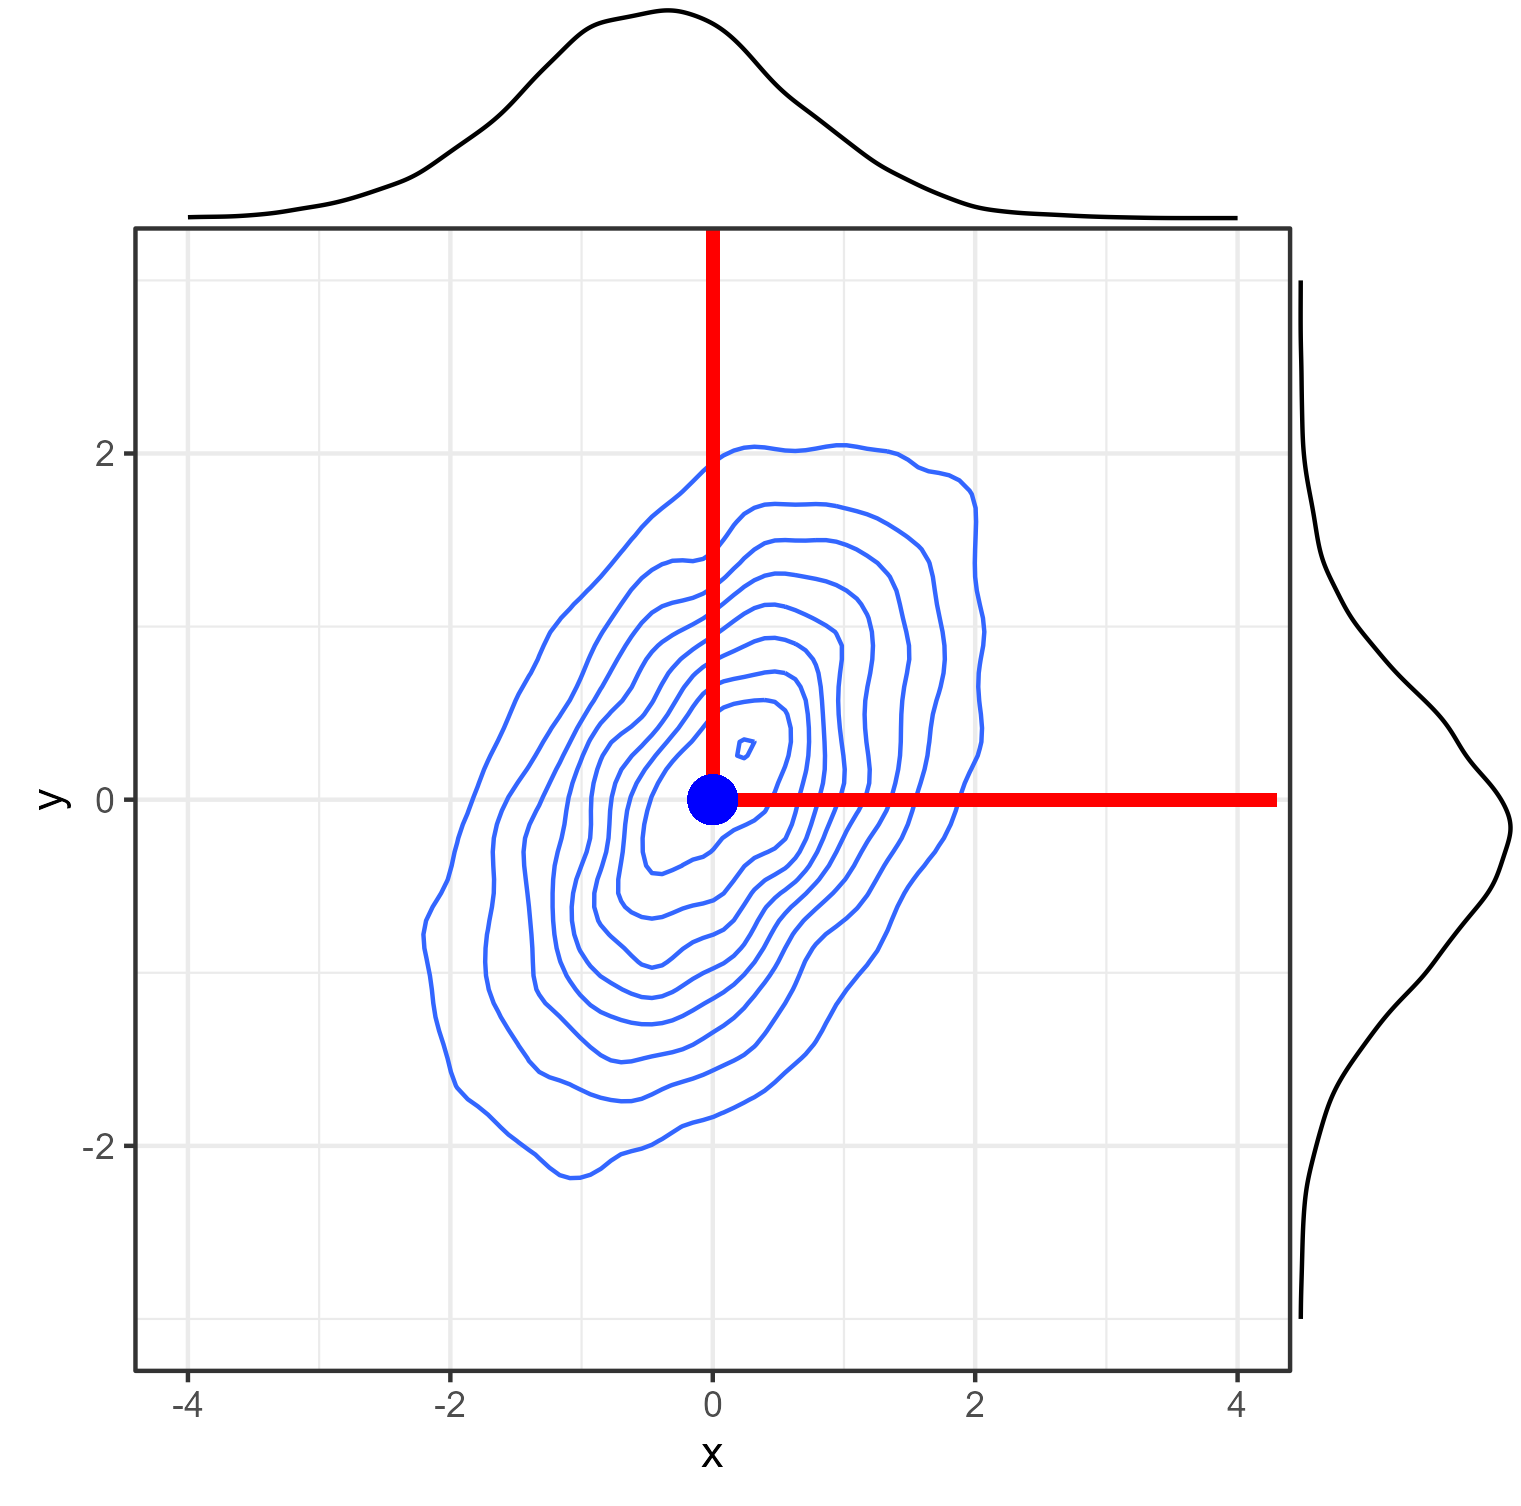
\includegraphics[scale=.6]{R/fixed-means}\end{center}
}

\frame{
\frametitle{A two input example}
\begin{center}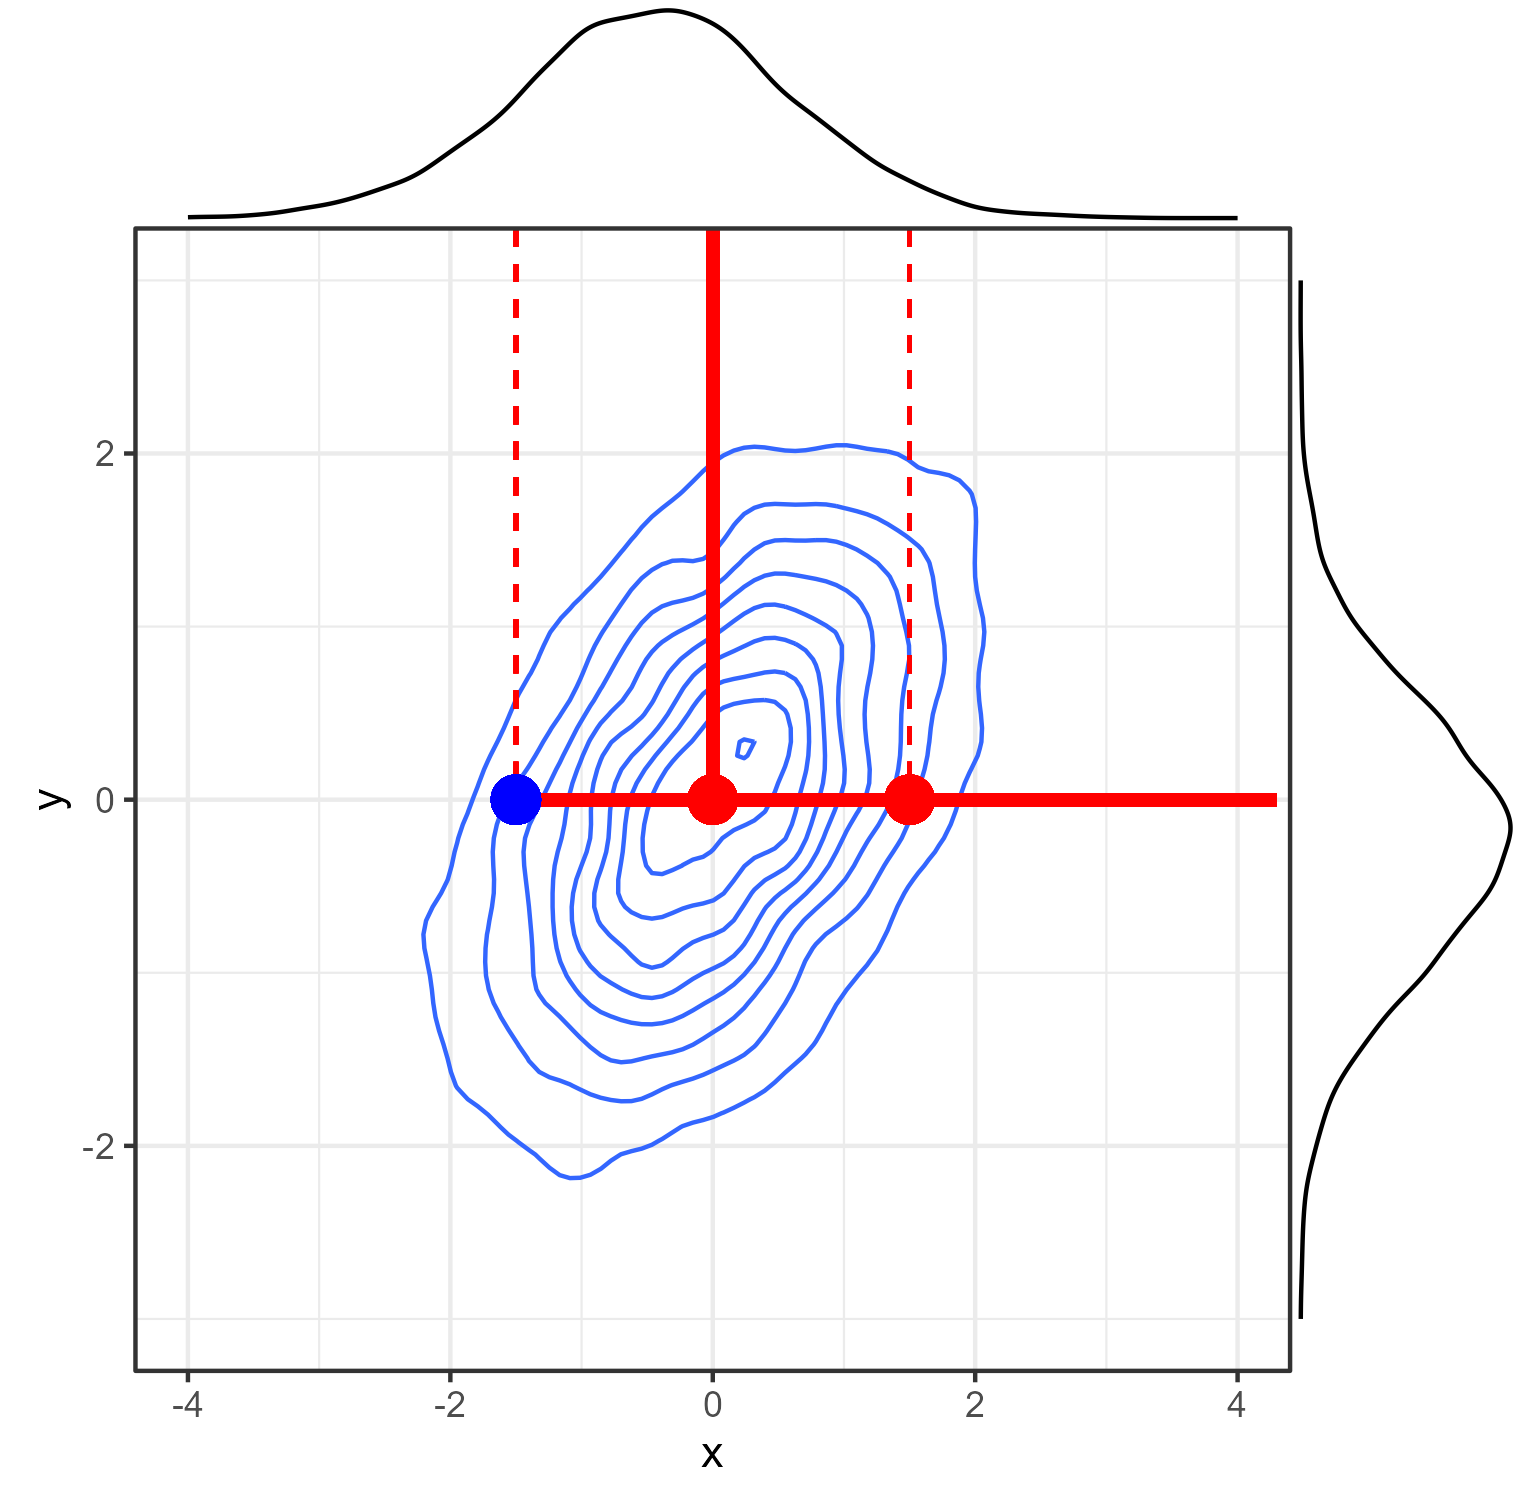
\includegraphics[scale=.6]{R/fixed-y-min}\end{center}
}

\frame{
\frametitle{A two input example}
\begin{center}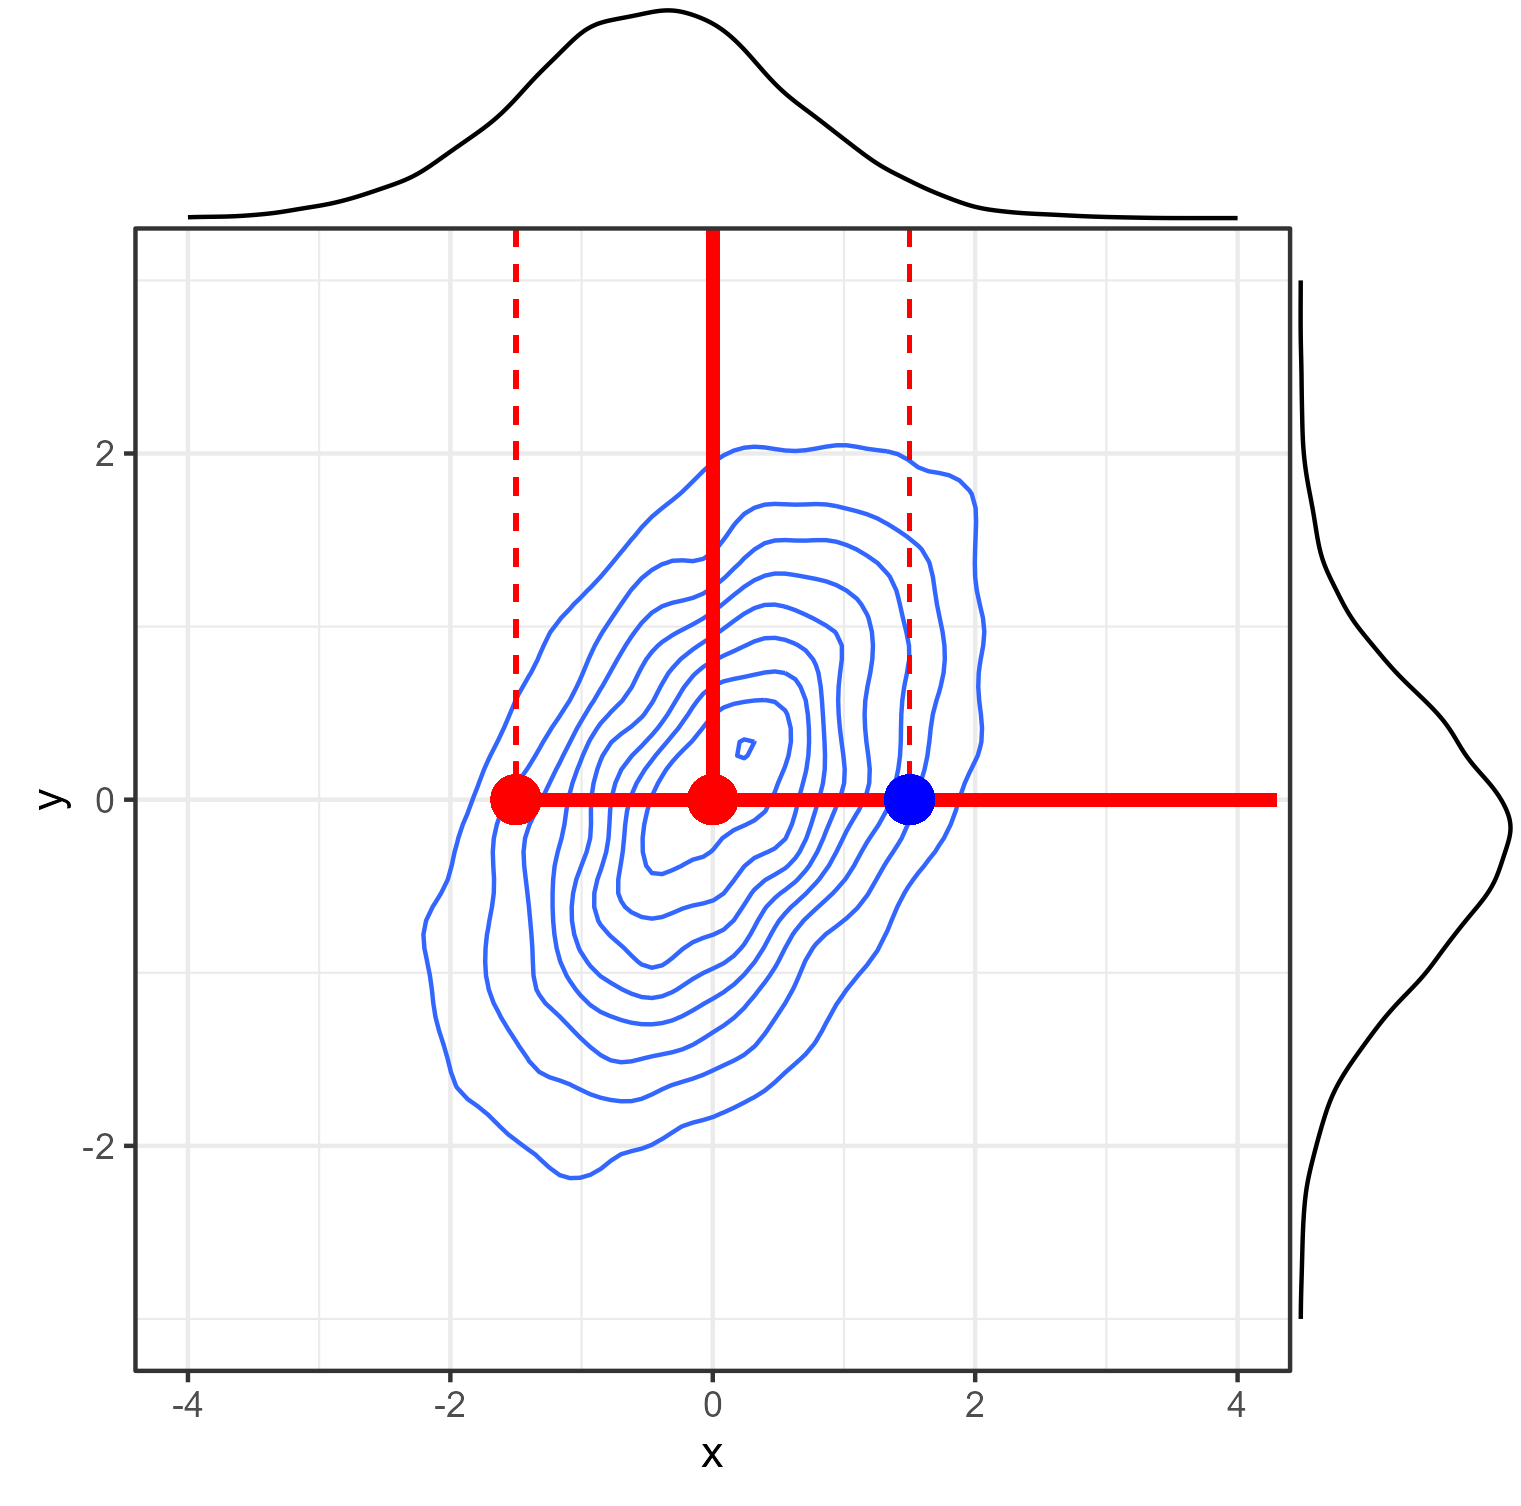
\includegraphics[scale=.6]{R/fixed-y-max}\end{center}
}

\frame{
\frametitle{A two input example}
\begin{center}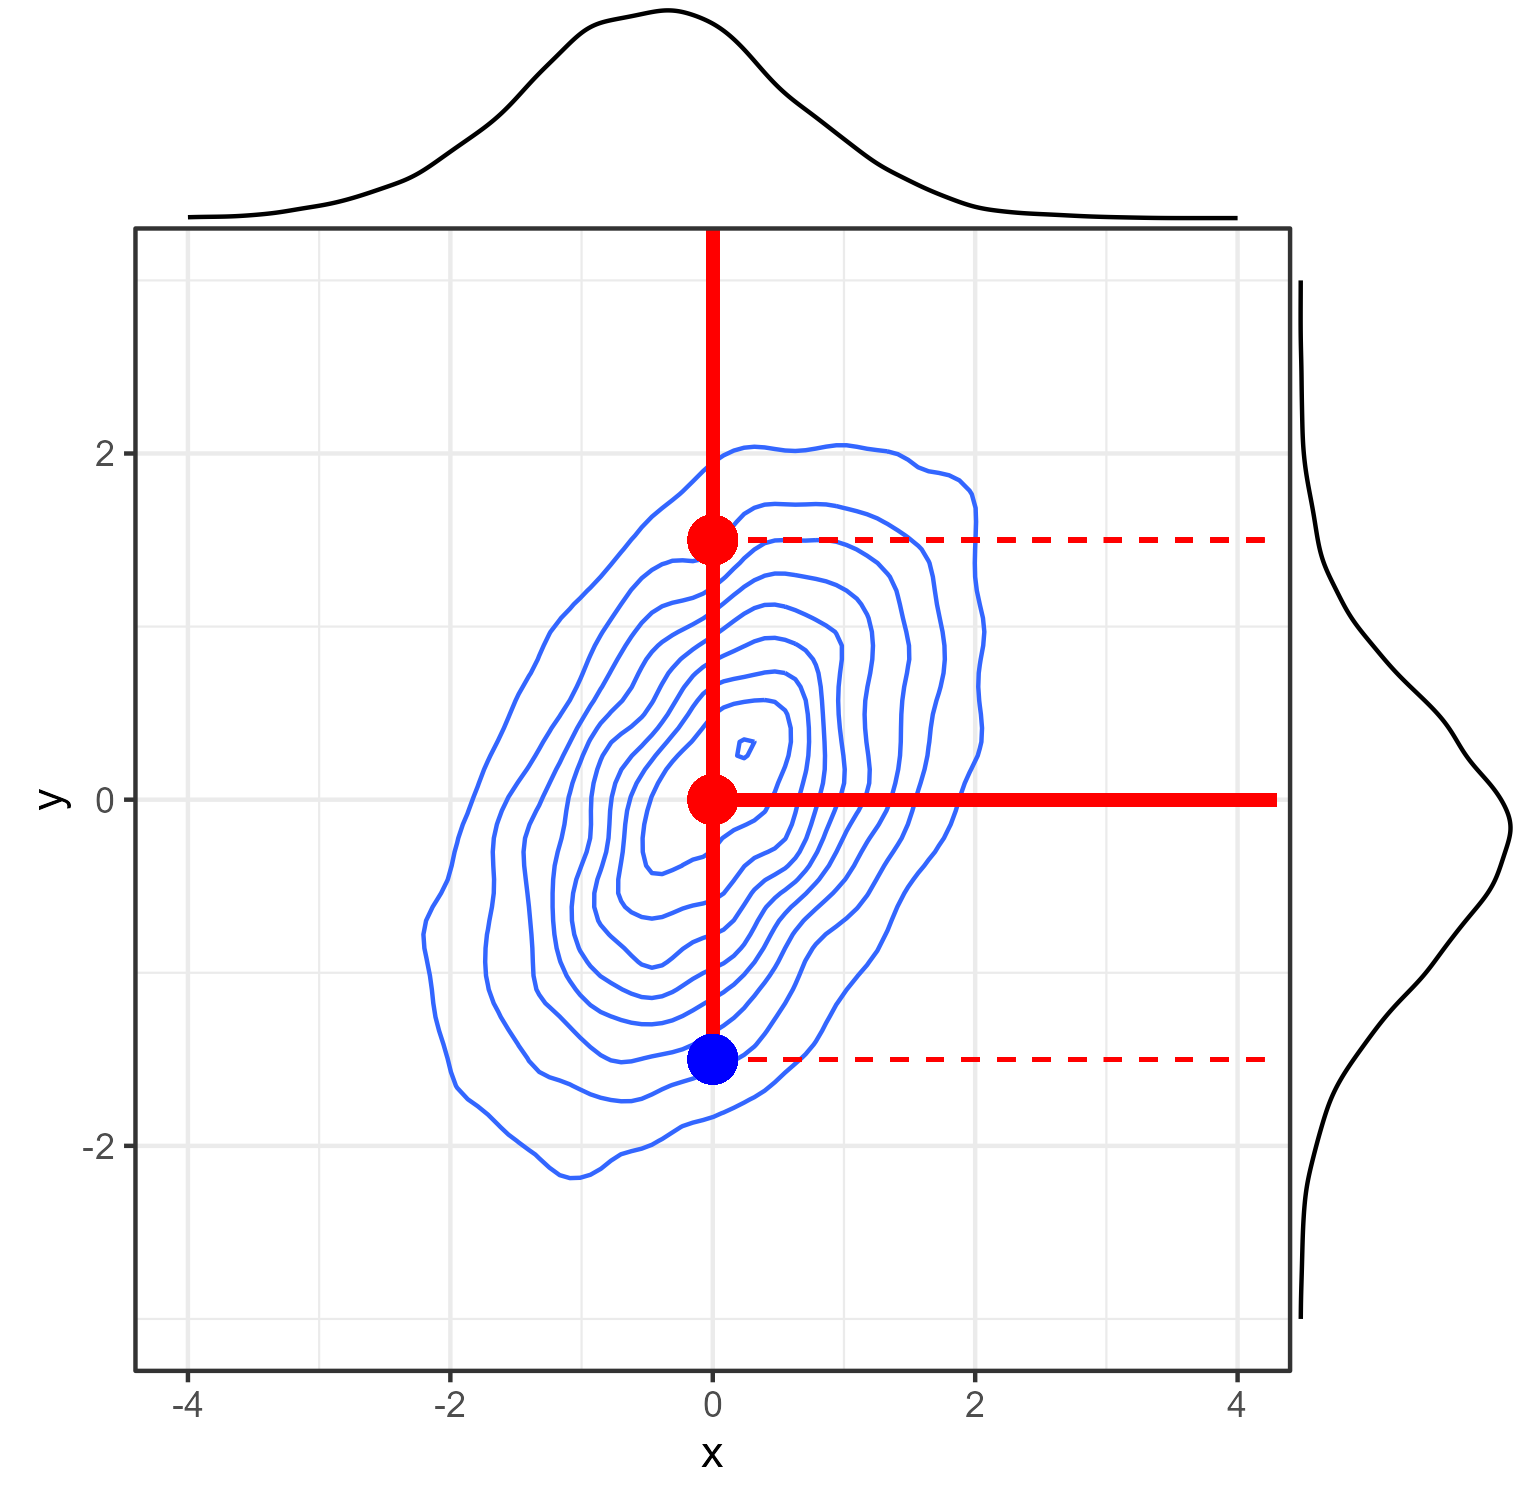
\includegraphics[scale=.6]{R/fixed-x-min}\end{center}
}

\frame{
\frametitle{A two input example}
\begin{center}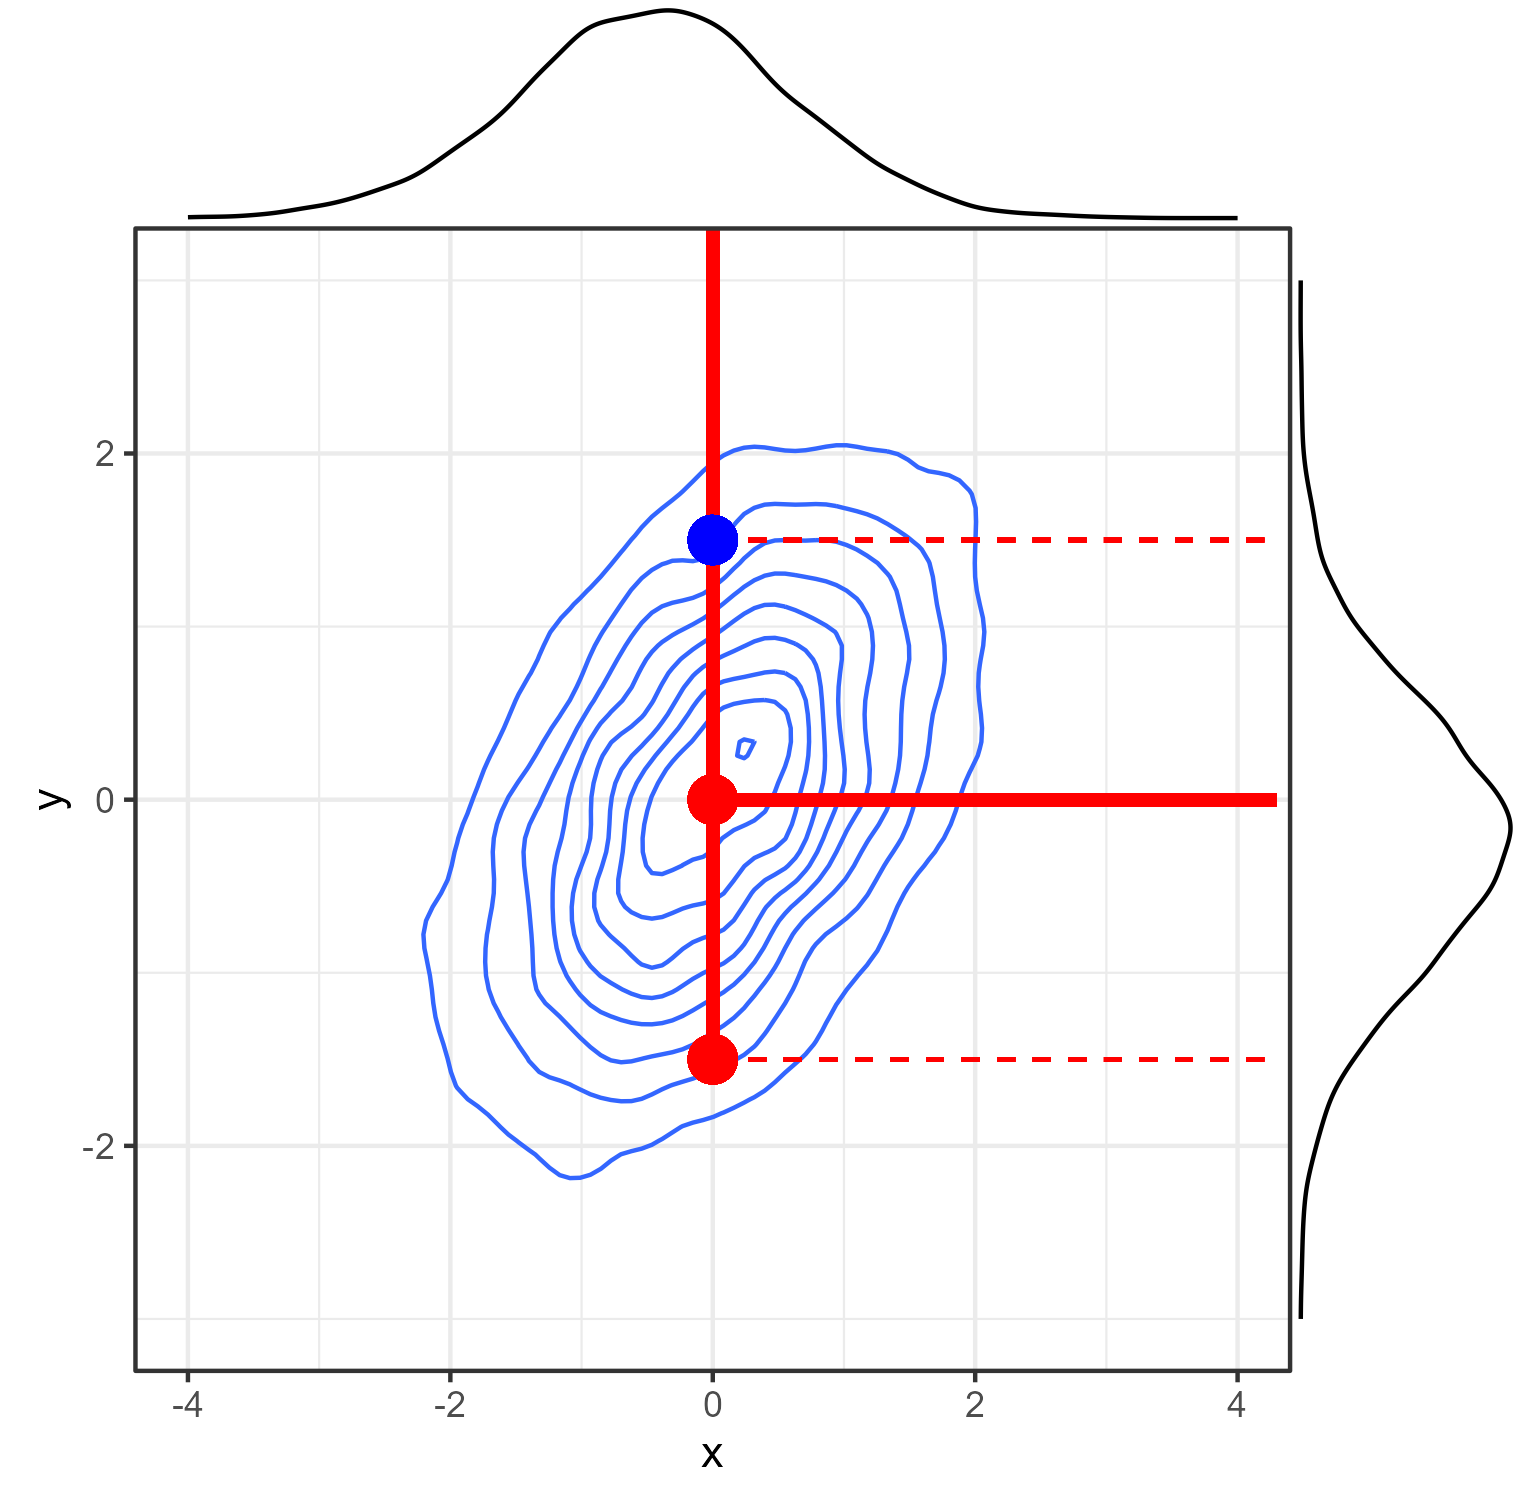
\includegraphics[scale=.6]{R/fixed-x-max}\end{center}
}

\frame{
\frametitle{A two input example}
\begin{center}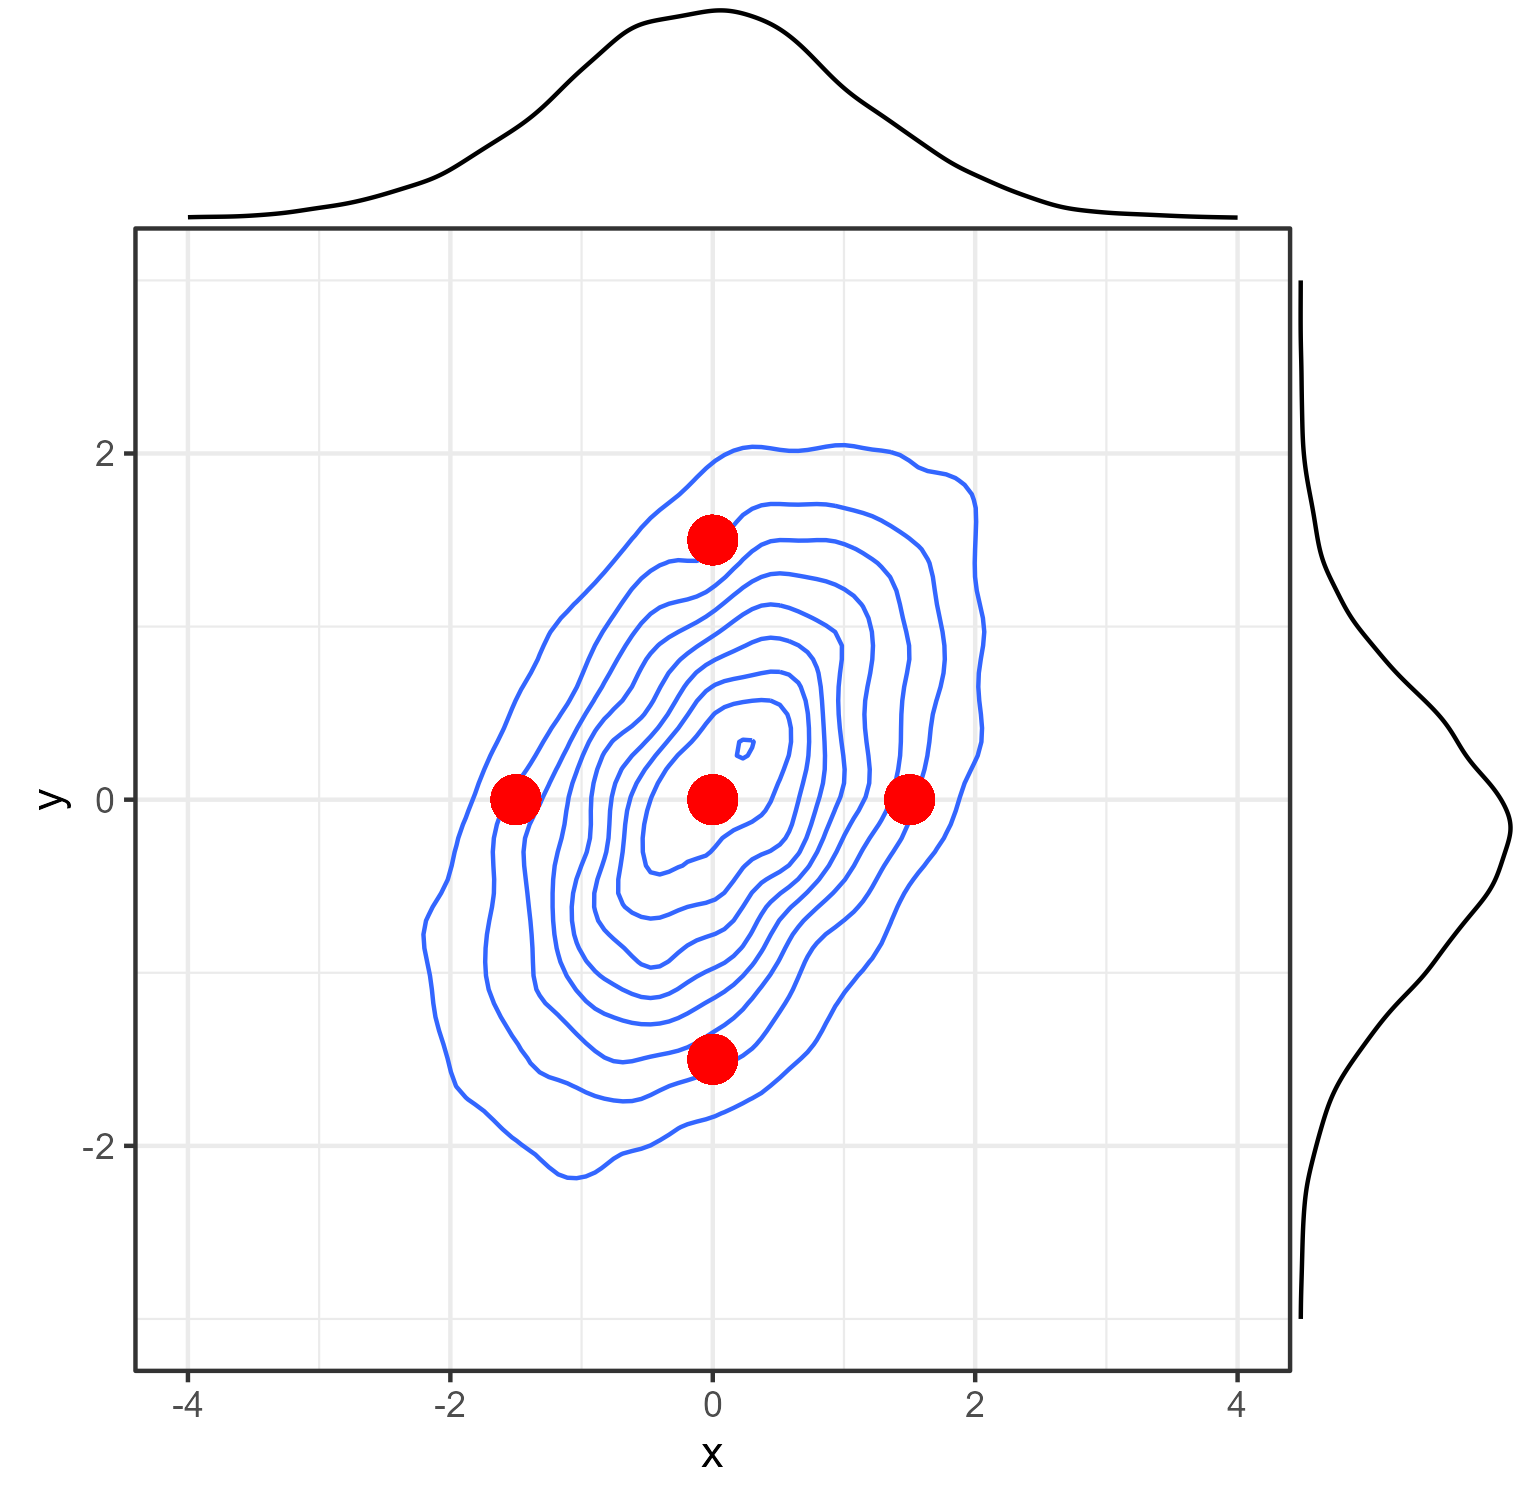
\includegraphics[scale=.6]{R/fixed-all}\end{center}
}

\frame{
\frametitle{A two input example}
\begin{center}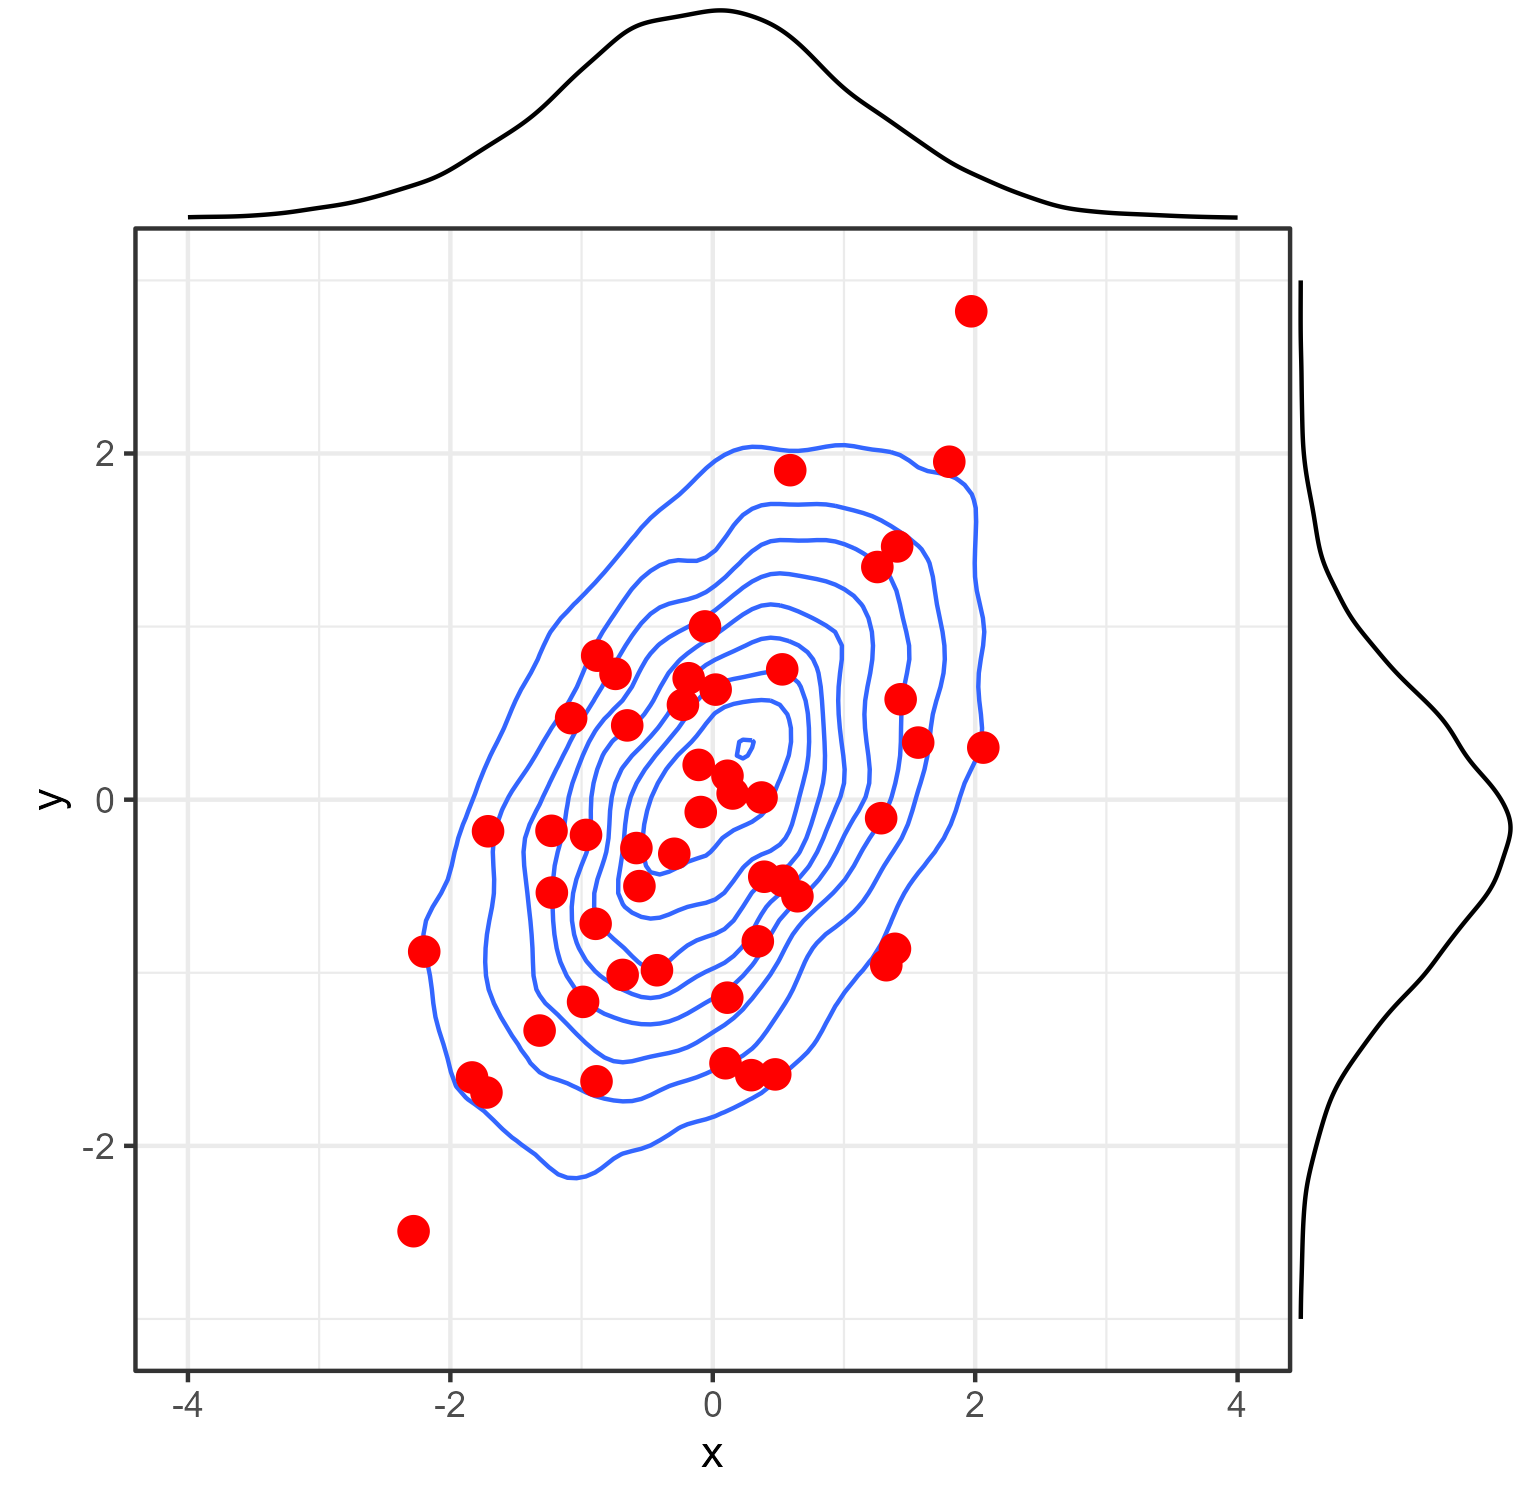
\includegraphics[scale=.6]{R/full-psa}\end{center}
}


% uncertainty propogation
\frame{
\frametitle{4.\ Uncertainty analysis}
\begin{overprint}
%%%\vspace{7pt}

%%%%%%%%%%%%%%%%%%%%%%%%%%%%%%%%%%%%%%%%%%%%%%%%%
\onslide<1|handout:0>
\fontsize{7}{8}\selectfont
\begin{tabular}{ccc}
\textbf{\blue Parameters} & \textbf{\blue Model structure} & \textbf{\blue Decision analysis} \\
\begin{minipage}[l]{2.5cm}
\begin{center}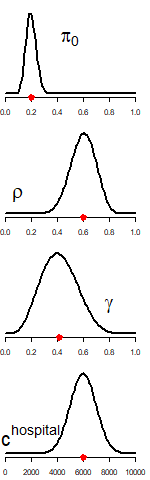
\includegraphics[scale=.37]{R/means-only}\end{center}
\end{minipage}
&
\begin{minipage}[l]{5cm}
\begin{center}\red{Old chemotherapy}\black\end{center}\vspace{-.5cm}
\begin{center}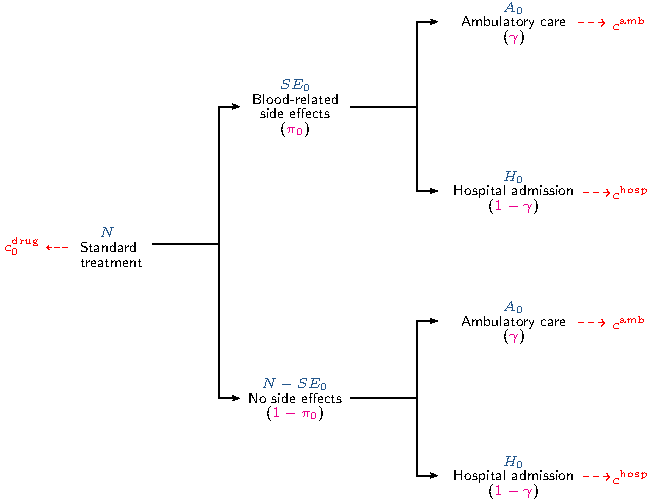
\includegraphics[scale=.37]{1.introduction-to-health-economic-evaluations/figs/ModelGraph2}\end{center}

\begin{center}\red{New chemotherapy}\black\end{center}\vspace{-.5cm}
\begin{center}\includegraphics[scale=.37]{1.introduction-to-health-economic-evaluations/figs/ModelGraph4}\end{center}
\end{minipage}
&
\begin{minipage}[l]{4cm}
\begin{tikzpicture}
\draw(2.5,2) node[align=center,draw=none]{
\begin{tabular}{cc}
\hline
\multicolumn{2}{c}{Old chemotherapy} \\
\hline
Benefits & Costs \\
\hline 
 &  \\
 &  \\
 &  \\
 &  \\
\hline
\textbf{\white 743.1} & \textbf{\white 656\,644.6} \\
\hline
\end{tabular}
};

\draw(2.5,-1) node[align=center,draw=none]{
\begin{tabular}{cc}
\hline
\multicolumn{2}{c}{New chemotherapy} \\
\hline
Benefits & Costs \\
\hline 
 &  \\
 &  \\
 &  \\
 &  \\
\hline
\textbf{\white 743.1} & \textbf{\white 656\,644.6} \\
\hline
\end{tabular}
};

\draw(2.5,-2.7) node(3){\white $\displaystyle \mbox{ICER} = \frac{\mbox{20\,000}}{\mbox{1QALY}}$\black};
\end{tikzpicture}
\end{minipage}
\end{tabular}


%%%%%%%%%%%%%%%%%%%%%%%%%%%%%%%%%%%%%%%%%%%%%%%%%
\onslide<2|handout:0>
\fontsize{7}{8}\selectfont
\begin{tabular}{ccc}
\textbf{\blue Parameters} & \textbf{\blue Model structure} & \textbf{\blue Decision analysis} \\
\begin{minipage}[l]{2.5cm}
\begin{center}\includegraphics[scale=.37]{R/max-min-pi}\end{center}
\end{minipage}
&
\begin{minipage}[l]{5cm}
\begin{center}\red{Old chemotherapy}\black\end{center}\vspace{-.5cm}
\begin{center}\includegraphics[scale=.37]{1.introduction-to-health-economic-evaluations/figs/ModelGraph2}\end{center}

\begin{center}\red{New chemotherapy}\black\end{center}\vspace{-.5cm}
\begin{center}\includegraphics[scale=.37]{1.introduction-to-health-economic-evaluations/figs/ModelGraph4}\end{center}
\end{minipage}
&
\begin{minipage}[l]{4cm}
\begin{tikzpicture}
\draw(2.5,2) node[align=center,draw=none]{
\begin{tabular}{cc}
\hline
\multicolumn{2}{c}{Old chemotherapy} \\
\hline
Benefits & Costs \\
\hline 
 &  \\
 &  \\
 &  \\
 &  \\
\hline
\textbf{\white 743.1} & \textbf{\white 656\,644.6} \\
\hline
\end{tabular}
};

\draw(2.5,-1) node[align=center,draw=none]{
\begin{tabular}{cc}
\hline
\multicolumn{2}{c}{New chemotherapy} \\
\hline
Benefits & Costs \\
\hline 
 &  \\
 &  \\
 &  \\
 &  \\
\hline
\textbf{\white 743.1} & \textbf{\white 656\,644.6} \\
\hline
\end{tabular}
};

\draw(2.5,-2.7) node(3){\white $\displaystyle \mbox{ICER} = \frac{\mbox{20\,000}}{\mbox{1QALY}}$\black};
\end{tikzpicture}
\end{minipage}
\end{tabular}

%%%%%%%%%%%%%%%%%%%%%%%%%%%%%%%%%%%%%%%%%%%%%%%%%
\onslide<3|handout:0>
\fontsize{7}{8}\selectfont
\begin{tabular}{ccc}
\textbf{\blue Parameters} & \textbf{\blue Model structure} & \textbf{\blue Decision analysis} \\
\begin{minipage}[l]{2.5cm}
\begin{center}\includegraphics[scale=.37]{R/max-min-rho}\end{center}
\end{minipage}
&
\begin{minipage}[l]{5cm}
\begin{center}\red{Old chemotherapy}\black\end{center}\vspace{-.5cm}
\begin{center}\includegraphics[scale=.37]{1.introduction-to-health-economic-evaluations/figs/ModelGraph2}\end{center}

\begin{center}\red{New chemotherapy}\black\end{center}\vspace{-.5cm}
\begin{center}\includegraphics[scale=.37]{1.introduction-to-health-economic-evaluations/figs/ModelGraph4}\end{center}
\end{minipage}
&
\begin{minipage}[l]{4cm}
\begin{tikzpicture}
\draw(2.5,2) node[align=center,draw=none]{
\begin{tabular}{cc}
\hline
\multicolumn{2}{c}{Old chemotherapy} \\
\hline
Benefits & Costs \\
\hline 
 &  \\
 &  \\
 &  \\
 &  \\
\hline
\textbf{\white 743.1} & \textbf{\white 656\,644.6} \\
\hline
\end{tabular}
};

\draw(2.5,-1) node[align=center,draw=none]{
\begin{tabular}{cc}
\hline
\multicolumn{2}{c}{New chemotherapy} \\
\hline
Benefits & Costs \\
\hline 
 &  \\
 &  \\
 &  \\
 &  \\
\hline
\textbf{\white 743.1} & \textbf{\white 656\,644.6} \\
\hline
\end{tabular}
};

\draw(2.5,-2.7) node(3){\white $\displaystyle \mbox{ICER} = \frac{\mbox{20\,000}}{\mbox{1QALY}}$\black};
\end{tikzpicture}
\end{minipage}
\end{tabular}

%%%%%%%%%%%%%%%%%%%%%%%%%%%%%%%%%%%%%%%%%%%%%%%%%
\onslide<4|handout:0>
\fontsize{7}{8}\selectfont
\begin{tabular}{ccc}
\textbf{\blue Parameters} & \textbf{\blue Model structure} & \textbf{\blue Decision analysis} \\
\begin{minipage}[l]{2.5cm}
\begin{center}\includegraphics[scale=.37]{R/max-min-gamma}\end{center}
\end{minipage}
&
\begin{minipage}[l]{5cm}
\begin{center}\red{Old chemotherapy}\black\end{center}\vspace{-.5cm}
\begin{center}\includegraphics[scale=.37]{1.introduction-to-health-economic-evaluations/figs/ModelGraph2}\end{center}

\begin{center}\red{New chemotherapy}\black\end{center}\vspace{-.5cm}
\begin{center}\includegraphics[scale=.37]{1.introduction-to-health-economic-evaluations/figs/ModelGraph4}\end{center}
\end{minipage}
&
\begin{minipage}[l]{4cm}
\begin{tikzpicture}
\draw(2.5,2) node[align=center,draw=none]{
\begin{tabular}{cc}
\hline
\multicolumn{2}{c}{Old chemotherapy} \\
\hline
Benefits & Costs \\
\hline 
 &  \\
 &  \\
 &  \\
 &  \\
\hline
\textbf{\white 743.1} & \textbf{\white 656\,644.6} \\
\hline
\end{tabular}
};

\draw(2.5,-1) node[align=center,draw=none]{
\begin{tabular}{cc}
\hline
\multicolumn{2}{c}{New chemotherapy} \\
\hline
Benefits & Costs \\
\hline 
 &  \\
 &  \\
 &  \\
 &  \\
\hline
\textbf{\white 743.1} & \textbf{\white 656\,644.6} \\
\hline
\end{tabular}
};

\draw(2.5,-2.7) node(3){\white $\displaystyle \mbox{ICER} = \frac{\mbox{20\,000}}{\mbox{1QALY}}$\black};
\end{tikzpicture}
\end{minipage}
\end{tabular}

%%%%%%%%%%%%%%%%%%%%%%%%%%%%%%%%%%%%%%%%%%%%%%%%%
\onslide<5|handout:0>
\fontsize{7}{8}\selectfont
\begin{tabular}{ccc}
\textbf{\blue Parameters} & \textbf{\blue Model structure} & \textbf{\blue Decision analysis} \\
\begin{minipage}[l]{2.5cm}
\begin{center}\includegraphics[scale=.37]{R/max-min-cost}\end{center}
\end{minipage}
&
\begin{minipage}[l]{5cm}
\begin{center}\red{Old chemotherapy}\black\end{center}\vspace{-.5cm}
\begin{center}\includegraphics[scale=.37]{1.introduction-to-health-economic-evaluations/figs/ModelGraph2}\end{center}

\begin{center}\red{New chemotherapy}\black\end{center}\vspace{-.5cm}
\begin{center}\includegraphics[scale=.37]{1.introduction-to-health-economic-evaluations/figs/ModelGraph4}\end{center}
\end{minipage}
&
\begin{minipage}[l]{4cm}
\begin{tikzpicture}
\draw(2.5,2) node[align=center,draw=none]{
\begin{tabular}{cc}
\hline
\multicolumn{2}{c}{Old chemotherapy} \\
\hline
Benefits & Costs \\
\hline 
 &  \\
 &  \\
 &  \\
 &  \\
\hline
\textbf{\white 743.1} & \textbf{\white 656\,644.6} \\
\hline
\end{tabular}
};

\draw(2.5,-1) node[align=center,draw=none]{
\begin{tabular}{cc}
\hline
\multicolumn{2}{c}{New chemotherapy} \\
\hline
Benefits & Costs \\
\hline 
 &  \\
 &  \\
 &  \\
 &  \\
\hline
\textbf{\white 743.1} & \textbf{\white 656\,644.6} \\
\hline
\end{tabular}
};

\draw(2.5,-2.7) node(3){\white $\displaystyle \mbox{ICER} = \frac{\mbox{20\,000}}{\mbox{1QALY}}$\black};
\end{tikzpicture}
\end{minipage}
\end{tabular}

% PSA
%%%%%%%%%%%%%%%%%%%%%%%%%%%%%%%%%%%%%%%
\onslide<6|handout:0>
\fontsize{7}{8}\selectfont
\begin{tabular}{ccc}
\textbf{\blue Parameters} & \textbf{\blue Model structure} & \textbf{\blue Decision analysis} \\
\begin{minipage}[l]{2.5cm}
\begin{center}\includegraphics[scale=.37]{R/psa-1}\end{center}
\end{minipage}
&
\begin{minipage}[l]{5cm}
\begin{center}\red{Old chemotherapy}\black\end{center}\vspace{-.5cm}
\begin{center}\includegraphics[scale=.37]{1.introduction-to-health-economic-evaluations/figs/ModelGraph2}\end{center}

\begin{center}\red{New chemotherapy}\black\end{center}\vspace{-.5cm}
\begin{center}\includegraphics[scale=.37]{1.introduction-to-health-economic-evaluations/figs/ModelGraph4}\end{center}
\end{minipage}
&
\begin{minipage}[l]{4cm}
\begin{tikzpicture}
\draw(2.5,2) node[align=center,draw=none]{
\begin{tabular}{cc}
\hline
\multicolumn{2}{c}{Old chemotherapy} \\
\hline
Benefits & Costs \\
\hline 
741 & 670\,382.1 \\
 &  \\
 &  \\
 &  \\
\hline
\textbf{\white 743.1} & \textbf{\white 656\,644.6} \\
\hline
\end{tabular}
};

\draw(2.5,-1) node[align=center,draw=none]{
\begin{tabular}{cc}
\hline
\multicolumn{2}{c}{New chemotherapy} \\
\hline
Benefits & Costs \\
\hline 
732 & 1\,131\,978 \\
 &  \\
 &  \\
 &  \\
\hline
\textbf{\white 743.1} & \textbf{\white 656\,644.6} \\
\hline
\end{tabular}
};

\draw(2.5,-2.7) node(3){\white $\displaystyle \mbox{ICER} = \frac{\mbox{20\,000}}{\mbox{1QALY}}$\black};
%\draw(-5.5,.3) node(4){$\Rightarrow$};
%\draw(-0,.3) node(5){$\Rightarrow$};
\end{tikzpicture}
\end{minipage}
\end{tabular}


%%%%%%%%%%%%%%%%%%%%%%%%%%%%%%%%%%%%%%%
\onslide<7|handout:0>
\fontsize{7}{8}\selectfont
\begin{tabular}{ccc}
\textbf{\blue Parameters} & \textbf{\blue Model structure} & \textbf{\blue Decision analysis} \\
\begin{minipage}[l]{2.5cm}
\begin{center}\includegraphics[scale=.37]{R/psa-2}\end{center}
\end{minipage}
&
\begin{minipage}[l]{5cm}
\begin{center}\red{Old chemotherapy}\black\end{center}\vspace{-.5cm}
\begin{center}\includegraphics[scale=.37]{1.introduction-to-health-economic-evaluations/figs/ModelGraph2}\end{center}

\begin{center}\red{New chemotherapy}\black\end{center}\vspace{-.5cm}
\begin{center}\includegraphics[scale=.37]{1.introduction-to-health-economic-evaluations/figs/ModelGraph4}\end{center}
\end{minipage}
&
\begin{minipage}[l]{4cm}
\begin{tikzpicture}
\draw(2.5,2) node[align=center,draw=none]{
\begin{tabular}{cc}
\hline
\multicolumn{2}{c}{Old chemotherapy} \\
\hline
Benefits & Costs \\
\hline 
741 & 670\,382.1 \\
699 & 871\,273.3 \\
 &  \\
 &  \\
\hline
 &  \\
\hline
\end{tabular}
};

\draw(2.5,-1) node[align=center,draw=none]{
\begin{tabular}{cc}
\hline
\multicolumn{2}{c}{New chemotherapy} \\
\hline
Benefits & Costs \\
\hline 
732 & 1\,131\,978 \\
664 & 1\,325\,654 \\
 &  \\
 &  \\
\hline
 &  \\
\hline
\end{tabular}
};

\draw(2.5,-2.7) node(3){\white $\displaystyle \mbox{ICER} = \frac{\mbox{20\,000}}{\mbox{1QALY}}$\black};
%\rput(-5.5,.3){$\Rightarrow$}
%\rput(-0,.3){$\Rightarrow$}
\end{tikzpicture}
\end{minipage}
\end{tabular}

%%%%%%%%%%%%%%%%%%%%%%%%%%%%%%%%%%%%%%%%%%%%%%%%%%%
\onslide<8|handout:1>
\fontsize{7}{8}\selectfont
\begin{tabular}{ccc}
\textbf{\blue Parameters} & \textbf{\blue Model structure} & \textbf{\blue Decision analysis} \\
\begin{minipage}[l]{2.5cm}
\begin{center}\includegraphics[scale=.37]{R/psa-3}\end{center}
\end{minipage}
&
\begin{minipage}[l]{5cm}
\begin{center}\red{Old chemotherapy}\black\end{center}\vspace{-.5cm}
\begin{center}\includegraphics[scale=.37]{1.introduction-to-health-economic-evaluations/figs/ModelGraph2}\end{center}

\begin{center}\red{New chemotherapy}\black\end{center}\vspace{-.5cm}
\begin{center}\includegraphics[scale=.37]{1.introduction-to-health-economic-evaluations/figs/ModelGraph4}\end{center}
\end{minipage}
&
\begin{minipage}[l]{4cm}
\begin{tikzpicture}
\draw(2.5,2) node[align=center,draw=none]{
\begin{tabular}{cc}
\hline
\multicolumn{2}{c}{Old chemotherapy} \\
\hline
Benefits & Costs \\
\hline 
741 & 670\,382.1 \\
699 & 871\,273.3 \\
$\ldots$ & $\ldots$ \\
726 & 425\,822.2 \\
\hline
\textbf{716.2} & \textbf{790\,381.2} \\
\hline
\end{tabular}
};

\draw(2.5,-1) node[align=center,draw=none]{
\begin{tabular}{cc}
\hline
\multicolumn{2}{c}{New chemotherapy} \\
\hline
Benefits & Costs \\
\hline 
732 & 1\,131\,978 \\
664 & 1\,325\,654 \\
$\ldots$ & $\ldots$ \\
811 & 766\,411.4 \\
\hline
\textbf{774.5} & \textbf{1\,066\,849.8} \\
\hline
\end{tabular}
};

\draw(2.5,-2.7) node(3){$\displaystyle \mbox{ICER} = \frac{\mbox{276\,468.6}}{\mbox{58.3}}$};
\draw(2.5,-3.2) node(3){$\displaystyle \mbox{\white ICER\black} = \mbox{6\,497.1}$};
%%%%
%%%%\rput(2,-2.7){$\displaystyle \mbox{ICER =} \frac{\mbox{276\,468.6}}{\mbox{58.3}}$}
%%%%\rput(2,-3.2){$\displaystyle \mbox{\white ICER\black =} \mbox{ 6\,497.1}$}
%%%%\rput(-5.5,.3){$\Rightarrow$}
%%%%\rput(-0,.3){$\Rightarrow$}
\end{tikzpicture}
\end{minipage}
\end{tabular}

\end{overprint}
}

\frame{
\frametitle{Is this \textit{all} we need? \hspace{0pt plus 1 filll}\small \textit{(see VoI)}}
\only<1-3|handout:1>{
\begin{itemize}
\item The CEAC only deals with the \textbf{\blue probability} of making the ``right decision''
\item But it does not account for the \textbf{\red payoff/penalty} associated with making the ``wrong''~one!
\vspace{10pt}
\item<2-3|handout:1> \textbf{Example 1}: Intervention $t=1$ is the most cost-effective, given current evidence
\begin{itemize}
\item<2-3|handout:1> \myblue $\Pr(\mbox{$t=1$ is cost-effective)}=$ 0.51 \black 
\item<2-3|handout:1> If we get it wrong: Increase in costs = \pounds 3
\item[]<2-3|handout:1> \white If we get it wrong: \black Decrease in effectiveness = 0.000001 QALYs
\item \red Large uncertainty\black/\color{blue!20!black!30!green} negligible consequences \black $\Rightarrow$ \textbf{\color{blue!20!black!30!green}can afford uncertainty}
\end{itemize}
\vspace{5pt}
\item<3|handout:1> \textbf{Example 2}: Intervention $t=1$ is the most cost-effective, given current evidence
\begin{itemize}
\item<3|handout:1> \myblue $\Pr(\mbox{$t=1$ is cost-effective)}=$ 0.999 \black 
\item<3|handout:1> If we get it wrong: Increase in costs = \pounds 1\,000\,000\,000
\item[]<3|handout:1> \white If we get it wrong: \black Decrease in effectiveness = 999999 QALYs
\item<3|handout:1> \color{blue!20!black!30!green} Tiny uncertainty\black/\red dire consequences \black $\Rightarrow$ \amber \textbf{probably should think about~it...}
\end{itemize}
\end{itemize}
}
}

 \nologo

%% customised footline for the final slide
\makeatletter
\setbeamertemplate{footline}{%
  \leavevmode%
  \hbox{%
  \begin{beamercolorbox}[wd=.35\paperwidth,ht=2.25ex,dp=1ex,center]{title in head/foot}%
    \usebeamerfont{title in head/foot}\insertshorttitle
  \end{beamercolorbox}%
  \begin{beamercolorbox}[wd=.10\paperwidth,ht=2.25ex,dp=1ex,center]{date in head/foot}% original wd=.15
    \usebeamerfont{date in head/foot}\insertshortdate{}
  \end{beamercolorbox}%
  \begin{beamercolorbox}[wd=.40\paperwidth,ht=2.25ex,dp=1ex,center]{section in head/foot}% original wd=.35
    \usebeamerfont{section in head/foot} \insertshortpart 
  \end{beamercolorbox}%
  \begin{beamercolorbox}[wd=.15\paperwidth,ht=2.25ex,dp=1ex,center]{date in head/foot}%
%    \insertframenumber{}\hspace*{1ex}(\insertpartstartpage--\insertpartendpage)
    \insertframenumber{}\hspace*{1ex}(\insertpartstartframe--\insertpartendframe)
  \end{beamercolorbox}}%
  \vskip0pt%
}


\end{document}
